\documentclass[nohyper,nobib,a4paper]{tufte-book}

% All the imports


\usepackage{nameref}
\usepackage{url}
\usepackage[T1]{fontenc}
\usepackage[utf8]{inputenc}
\usepackage[backend=biber, natbib=true, style=numeric]{biblatex}
\usepackage{polski}

\usepackage{tikz}
\usepackage{tabularx}
\usepackage{colortbl}
\usepackage{xltabular}
\usepackage{placeins}
\usepackage{xargs}
\usepackage{hyperref}

%\newcounter{counterC}
%\newcommand{\countC}{%
%   \stepcounter{counterC}%
%   \thertaskno}

\renewcommandx{\cite}[3][1={0pt},2={}]{\sidenote[][#1]{\fullcite[#2]{#3}}}
\newcommandx{\citeC}[3][1={0pt},2={}]{{\color{red}[#3]}\marginnote[#1]{\color{red}[#3]\\\vspace{-.5em}\noindent\hrulefill\\\noindent\fullcite[#2]{#3}\\\vspace{-.5em}\noindent\hrulefill}}

\newcommandx{\citeZ}[3][1={0pt},2={}]{{~{\color{black!100}[#3]}}\marginnote[#1]{\color{black!100}[#3]~\scriptsize\fullcite[#2]{#3}}}

\newcommandx{\citeM}[3][1={0pt},2={}]{{\color{blue}[#3]}\marginnote[#1]{\color{blue}[#3]~\scriptsize\fullcite[#2]{#3}}}


%%
% For nicely typeset tabular material
\usepackage{booktabs}

%%
% For graphics / images
\usepackage{graphicx}
\setkeys{Gin}{width=\linewidth,totalheight=\textheight,keepaspectratio}
\graphicspath{{graphics/}}
\graphicspath{{figures/}}

% The fancyvrb package lets us customize the formatting of verbatim
% environments.  We use a slightly smaller font.
\usepackage{fancyvrb}
\fvset{fontsize=\normalsize}

%%
% Prints argument within hanging parentheses (i.e., parentheses that take
% up no horizontal space).  Useful in tabular environments.
\newcommand{\hangp}[1]{\makebox[0pt][r]{(}#1\makebox[0pt][l]{)}}

%%
% Prints an asterisk that takes up no horizontal space.
% Useful in tabular environments.
\newcommand{\hangstar}{\makebox[0pt][l]{*}}

%%
% Prints a trailing space in a smart way.
\usepackage{xspace}

%%
% Some shortcuts for Tufte's book titles.  The lowercase commands will
% produce the initials of the book title in italics.  The all-caps commands
% will print out the full title of the book in italics.
\newcommand{\vdqi}{\textit{VDQI}\xspace}
\newcommand{\ei}{\textit{EI}\xspace}
\newcommand{\ve}{\textit{VE}\xspace}
\newcommand{\be}{\textit{BE}\xspace}
\newcommand{\VDQI}{\textit{The Visual Display of Quantitative Information}\xspace}
\newcommand{\EI}{\textit{Envisioning Information}\xspace}
\newcommand{\VE}{\textit{Visual Explanations}\xspace}
\newcommand{\BE}{\textit{Beautiful Evidence}\xspace}

\newcommand{\TL}{Tufte-\LaTeX\xspace}

% Prints the month name (e.g., January) and the year (e.g., 2008)
\newcommand{\monthyear}{%
  \ifcase\month\or January\or February\or March\or April\or May\or June\or
  July\or August\or September\or October\or November\or
  December\fi\space\number\year
}

% Prints an epigraph and speaker in sans serif, all-caps type.
\newcommand{\openepigraph}[2]{%
  %\sffamily\fontsize{14}{16}\selectfont
  \begin{fullwidth}
  \sffamily\large
  \begin{doublespace}
  \noindent\allcaps{#1}\\% epigraph
  \noindent\allcaps{#2}% author
  \end{doublespace}
  \end{fullwidth}
}

% Inserts a blank page
\newcommand{\blankpage}{\newpage\hbox{}\thispagestyle{empty}\newpage}

\usepackage{units}

% Typesets the font size, leading, and measure in the form of 10/12x26 pc.
\newcommand{\measure}[3]{#1/#2$\times$\unit[#3]{pc}}

% Macros for typesetting the documentation
\newcommand{\hlred}[1]{\textcolor{Maroon}{#1}}% prints in red
\newcommand{\hangleft}[1]{\makebox[0pt][r]{#1}}
\newcommand{\hairsp}{\hspace{1pt}}% hair space
\newcommand{\hquad}{\hskip0.5em\relax}% half quad space
\newcommand{\TODO}{\textcolor{red}{\bf TODO!}\xspace}
\newcommand{\ie}{\textit{i.\hairsp{}e.}\xspace}
\newcommand{\eg}{\textit{e.\hairsp{}g.}\xspace}
\newcommand{\na}{\quad--}% used in tables for N/A cells
\providecommand{\XeLaTeX}{X\lower.5ex\hbox{\kern-0.15em\reflectbox{E}}\kern-0.1em\LaTeX}
\newcommand{\tXeLaTeX}{\XeLaTeX\index{XeLaTeX@\protect\XeLaTeX}}
% \index{\texttt{\textbackslash xyz}@\hangleft{\texttt{\textbackslash}}\texttt{xyz}}
\newcommand{\tuftebs}{\symbol{'134}}% a backslash in tt type in OT1/T1
\newcommand{\doccmdnoindex}[2][]{\texttt{\tuftebs#2}}% command name -- adds backslash automatically (and doesn't add cmd to the index)
\newcommand{\doccmddef}[2][]{%
  \hlred{\texttt{\tuftebs#2}}\label{cmd:#2}%
  \ifthenelse{\isempty{#1}}%
    {% add the command to the index
      \index{#2 command@\protect\hangleft{\texttt{\tuftebs}}\texttt{#2}}% command name
    }%
    {% add the command and package to the index
      \index{#2 command@\protect\hangleft{\texttt{\tuftebs}}\texttt{#2} (\texttt{#1} package)}% command name
      \index{#1 package@\texttt{#1} package}\index{packages!#1@\texttt{#1}}% package name
    }%
}% command name -- adds backslash automatically
\newcommand{\doccmd}[2][]{%
  \texttt{\tuftebs#2}%
  \ifthenelse{\isempty{#1}}%
    {% add the command to the index
      \index{#2 command@\protect\hangleft{\texttt{\tuftebs}}\texttt{#2}}% command name
    }%
    {% add the command and package to the index
      \index{#2 command@\protect\hangleft{\texttt{\tuftebs}}\texttt{#2} (\texttt{#1} package)}% command name
      \index{#1 package@\texttt{#1} package}\index{packages!#1@\texttt{#1}}% package name
    }%
}% command name -- adds backslash automatically
\newcommand{\docopt}[1]{\ensuremath{\langle}\textrm{\textit{#1}}\ensuremath{\rangle}}% optional command argument
\newcommand{\docarg}[1]{\textrm{\textit{#1}}}% (required) command argument
\newenvironment{docspec}{\begin{quotation}\ttfamily\parskip0pt\parindent0pt\ignorespaces}{\end{quotation}}% command specification environment
\newcommand{\docenv}[1]{\texttt{#1}\index{#1 environment@\texttt{#1} environment}\index{environments!#1@\texttt{#1}}}% environment name
\newcommand{\docenvdef}[1]{\hlred{\texttt{#1}}\label{env:#1}\index{#1 environment@\texttt{#1} environment}\index{environments!#1@\texttt{#1}}}% environment name
\newcommand{\docpkg}[1]{\texttt{#1}\index{#1 package@\texttt{#1} package}\index{packages!#1@\texttt{#1}}}% package name
\newcommand{\doccls}[1]{\texttt{#1}}% document class name
\newcommand{\docclsopt}[1]{\texttt{#1}\index{#1 class option@\texttt{#1} class option}\index{class options!#1@\texttt{#1}}}% document class option name
\newcommand{\docclsoptdef}[1]{\hlred{\texttt{#1}}\label{clsopt:#1}\index{#1 class option@\texttt{#1} class option}\index{class options!#1@\texttt{#1}}}% document class option name defined
\newcommand{\docmsg}[2]{\bigskip\begin{fullwidth}\noindent\ttfamily#1\end{fullwidth}\medskip\par\noindent#2}
\newcommand{\docfilehook}[2]{\texttt{#1}\index{file hooks!#2}\index{#1@\texttt{#1}}}
\newcommand{\doccounter}[1]{\texttt{#1}\index{#1 counter@\texttt{#1} counter}}

% Generates the index
\usepackage{makeidx}
\makeindex

\usepackage{eso-pic,xcolor}

%%%% Kevin Godny's code for title page and contents from https://groups.google.com/forum/#!topic/tufte-latex/ujdzrktC1BQ
\makeatletter
\renewcommand{\maketitlepage}{%
\AddToShipoutPictureBG*{%
  \AtPageLowerLeft{%
    %\vspace*{.5\paperheight}%
    \color{red}%
    \rule{\paperwidth}{.38\paperheight}%
  }%
}%

\begingroup%
\setlength{\parindent}{0pt}

{\color{red}\fontsize{18}{18}\selectfont\textit{dr inż. \@author}\par}

\vspace{1.75in}{\color{red}\fontsize{24}{32}\selectfont\@title\par}

\vspace{0.5in}{\color{red}\fontsize{14}{14}\selectfont\textsf{\smallcaps{\@date}}\par}

\vfill{\fontsize{11}{11}\selectfont\textit{\@publisher}\par}
\thispagestyle{empty}
\endgroup
}
\makeatother

\titlecontents{part}%
    [0pt]% distance from left margin
    {\addvspace{0.25\baselineskip}}% above (global formatting of entry)
    {\allcaps{Part~\thecontentslabel}\allcaps}% before w/ label (label = ``Part I'')
    {\allcaps{Part~\thecontentslabel}\allcaps}% before w/o label
    {}% filler and page (leaders and page num)
    [\vspace*{0.5\baselineskip}]% after

\titlecontents{chapter}%
    [4em]% distance from left margin
    {}% above (global formatting of entry)
    {\contentslabel{2em}\textit}% before w/ label (label = ``Chapter 1'')
    {\hspace{0em}\textit}% before w/o label
    {\qquad\thecontentspage}% filler and page (leaders and page num)
    [\vspace*{0.5\baselineskip}]% after
%%%% End additional code by Kevin Godby

\setcounter{secnumdepth}{2}
%\geometry{textwidth=.6\paperwidth}

\geometry{
  left=19.8mm, % left margin
  textwidth=115mm, % main text block
  marginparsep=8.2mm, % gutter between main text block and margin notes
  marginparwidth=35mm % width of margin notes
}

\def\thesection{\arabic{section}}

\usepackage[polish]{babel}
\usepackage[Lenny]{fncychap}

%\usepackage[Lenny]{fncychap}
\renewcommand{\chaptername}{Załącznik}

\addto\captionspolish{\renewcommand{\chaptername}{Zalacznik}}

\ChNameUpperCase
\ChNumVar{\fontsize{40}{42}\usefont{OT1}{ptm}{m}{n}\selectfont}
%\ChTitleVar{\LARGE\sc}

%
%\usepackage[backend=biber, natbib=true, defernumbers=true]{biblatex}

%\newcounter{bbx:primcount}
%\setcounter{bbx:primcount}{0}


% Count number of  primary entries; expand labelnumberwidth
% to accommodate suffixes (NB: this might need tweaking when there
% are relatively many more secondary entries)
%\makeatletter
%\AtDataInput{%
%  \ifkeyword{secondary}
%    {}
%    {\addtocounter{bbx:primcount}{1}%
%     \blx@setlabwidth{\labelnumberwidth}{%
%       \csuse{abx@ffd@*@labelnumberwidth}{\thefield{labelnumber}a}}}}
%\makeatother

% Print labelnumbers with suffixes, adjust secondary labelnumber
%\DeclareFieldFormat{labelnumber}{%
%  \ifkeyword{secondary}
%    {{\number\numexpr#1-\value{bbx:primcount}}b}
%    {#1a}}
    
%%
% Book metadata
\title{\nohyphenation Projektowanie algorytmów rozpoznawania wzorców dla zadania klasyfikacji trudnych~danych}
\date{\nohyphenation Wniosek o~przeprowadzenie postępowania w~sprawie nadania stopnia doktora habilitowanego wraz z~załącznikami}
\author{Paweł Ksieniewicz}
\publisher{~}%Dyscyplina naukowa:\\\textbf{Informatyka Techniczna i Telekomunikacja}}

\definecolor{red}{RGB}{175, 30, 30}
\definecolor{green}{RGB}{30, 175, 30}
\definecolor{blue}{RGB}{30, 30, 175}
\newcommand*{\mybox}[1]{\fcolorbox{white}{red!10}{\small\color{black}\bfseries\strut#1}}
\usepackage{comment}

% Literatura, rozbita na trzy zakresy.
\addbibresource{cykl.bib}
\addbibresource{bibliography.bib}
\addbibresource{external.bib}

\usepackage{pdfpages}

\begin{document}


% Front matter
\frontmatter

\mainmatter




% r.1 blank page
%\blankpage

% v.2 epigraphs
%\newpage\thispagestyle{empty}
%\openepigraph{Są efekty.}{Michał Woźniak}
%\vfill
%\newpage

% r.3 full title page
\maketitle
%\blankpage

% v.4 copyright page
%\newpage
%\begin{fullwidth}
%~\vfill
%\thispagestyle{empty}
%\setlength{\parindent}{0pt}
%\setlength{\parskip}{\baselineskip}
%Copyright \copyright\ \the\year\ \thanklessauthor

%\par\smallcaps{Published by \thanklesspublisher}

%\par\smallcaps{tufte-latex.googlecode.com}

%\par Licensed under the Apache License, Version 2.0 (the ``License''); you may not
%use this file except in compliance with the License. You may obtain a copy
%of the License at \url{http://www.apache.org/licenses/LICENSE-2.0}. Unless
%required by applicable law or agreed to in writing, software distributed
%under the License is distributed on an \smallcaps{``AS IS'' BASIS, WITHOUT
%WARRANTIES OR CONDITIONS OF ANY KIND}, either express or implied. See the
%License for the specific language governing permissions and limitations
%under the License.\index{license}

%\par\textit{First printing, \monthyear}
%\end{fullwidth}

% r.5 contents
%\tableofcontents
%\listoffigures
%\listoftables

% r.7 dedication
%\cleardoublepage
%~\vfill
%\begin{doublespace}
%\noindent\fontsize{18}{22}\selectfont\itshape
%\nohyphenation
%Dedicated to those who appreciate \LaTeX{} 
%and the work of \mbox{Edward R.~Tufte} 
%and \mbox{Donald E.~Knuth}.
%\end{doublespace}
%\vfill
%\vfill

%\blankpage
\newpage
\thispagestyle{empty}
\begin{fullwidth}
	
\hspace{.75\textwidth}
\begin{minipage}{.65\textwidth}
\textbf{Politechnika Wrocławska}\\
Wybrzeże Wyspiańskiego 27\\
50-370 Wrocław\\
Dyscyplina naukowa: \textbf{Informatyka Techniczna i Telekomunikacja}\\
\underline{za pośrednictwem:}\\
\textbf{Rady Doskonałości Naukowej}\\
pl. Defilad 1\\
00-901 Warszawa\\
(Pałac Kultury i Nauki, p. XXIV, pok. 2401)
\end{minipage}

\noindent\begin{minipage}{.75\textwidth}
\textbf{Paweł Ksieniewicz}\\
\textbf{Politechnika Wrocławska}\\
\textbf{Wydział Informatyki i Telekomunikacji}\\
\textbf{Katedra Systemów i Sieci Komputerowych}\\
Wybrzeże Wyspiańskiego 27\\
50-370 Wrocław
\end{minipage}
\vspace{1em}

\begin{center}
	{\textbf{\large Wniosek}}
	
	z dnia 27.08.2022	
\end{center}

o przeprowadzenie postępowania w sprawie nadania stopnia doktora habilitowanego w dziedzinie \textbf{Nauk inżynieryjno-technicznych} w dyscyplinie$^1$ \textbf{Informatyka techniczna i telekomunikacja}.\vspace{1em}

\hspace{3em}\begin{minipage}{45em}
Określenie osiągnięcia naukowego będącego podstawą ubiegania się o nadanie stopnia doktora habilitowanego: cykl publikacji naukowych zatytułowany „\textbf{Projektowanie algorytmów rozpoznawania wzorców dla zadania klasyfikacji trudnych danych}”.
\end{minipage}\vspace{1em}

\noindent Wnioskuję -- na podstawie art. 221 ust. 10 ustawy z dnia 20 lipca 2018 r. Prawo o szkolnictwie wyższym i nauce (Dz. U. z 2021 r. poz. 478 zm.) – aby komisja habilitacyjna podejmowała uchwałę w~sprawie nadania stopnia doktora habilitowanego w głosowaniu \textbf{jawnym}$^{*2}$.\vspace{1em}

\begin{minipage}{45em}
\it
Zostałem poinformowany, że:

Administratorem w odniesieniu do danych osobowych pozyskanych w ramach postępowania w sprawie nadania stopnia doktora habilitowanego jest Przewodniczący Rady Doskonałości Naukowej z siedzibą w Warszawie (pl. Defilad 1, XXIV piętro, 00-901 Warszawa).

Kontakt za pośrednictwem e-mail: \url{kancelaria@rdn.gov.pl}, tel. 22 656 60 98 lub w siedzibie organu. Dane osobowe będą przetwarzane w oparciu o przesłankę wskazaną w art. 6 ust. 1 lit. c) Rozporządzenia UE 2016/679 z dnia z dnia 27 kwietnia 2016 r. w związku z art. 220 - 221 orazart. 232 – 240 ustawy z dnia 20 lipca 2018 roku - Prawo o szkolnictwie wyższym i nauce, w celu przeprowadzenie postępowania o nadanie stopnia doktora habilitowanego oraz realizacji praw i obowiązków oraz środków odwoławczych przewidzianych w tym postępowaniu.

Szczegółowa informacja na temat przetwarzania danych osobowych w postępowaniu dostępna jest na stronie \url{www.rdn.gov.pl/klauzula-informacyjna-rodo.html}
\end{minipage}

\vspace{5em}
\vfill\noindent\hspace{.75\textwidth}\begin{minipage}{15em}
\begin{center}
	\hbox to 5cm{\leaders\hbox to 3pt{\hss . \hss}\hfil}

	(podpis wnioskodawcy)
\end{center}
\end{minipage}

\vfill\noindent\begin{minipage}{50em}
\footnotesize\rule{15em}{.5pt}

$^{1}$ Klasyfikacja dziedzin i dyscyplin wg. rozporządzenia Ministra Nauki i Szkolnictwa Wyższego z dnia 20 września 2018 r. w sprawie dziedzin nauki i dyscyplin naukowych oraz dyscyplin w zakresie sztuki (Dz. U. z 2018 r. poz. 1818).

$^{2*}$ Niepotrzebne skreślić.
	
\end{minipage}

\newpage
\thispagestyle{empty}

\underline{Załączniki}:
\begin{enumerate}
	\item Dane wnioskodawcy
	\item Kopia dokumentu potwierdzającego posiadanie stopnia doktora
	\item Autoreferat wnioskodawcy
	\item Wykaz osiągnięć naukowych
	\item Deklaracje współautorów dotyczące wkładu pracy
	\item Publikacje wchodzące w skład osiągnięcia naukowego „Projektowanie algorytmów rozpoznawania wzorców dla zadania klasyfikacji danych trudnych”
	%\item Inne wybrane publikacje naukowe
\end{enumerate}

\end{fullwidth}


%\blankpage
\thispagestyle{empty}
\begin{fullwidth}

\chapter{Dane wnioskodawcy}

%\begin{center}
%	{\textbf{\large Dane wnioskodawcy}}	
%\end{center}

\vfill
{
\large
\begin{enumerate}
	\item Imię i Nazwisko: \emph{Paweł Ksieniewicz}
	\item Miejsce pracy: \emph{Katedra Systemów i Sieci Komputerowych, Wydział Informatyki i Telekomunikacji, Politechnika Wrocławska}
	\item Adres korespondencyjny: \emph{ul. Xxxxxxxxx xxb/XXa, xx-xxx Wrocław}
	\item Nr telefonu: \emph{XXX XXX XXX}
	\item Adres e-mail: \emph{XXXXX.XXXXXXXXXXX@pwr.edu.pl}
	\item Numer PESEL: \emph{XXXXXXXXXXX}
	\item Numer i seria dokumentu tożsamości w przypadku braku nadania numeru PESEL:
	\item[]~ \hbox to 15cm{\leaders\hbox to 3pt{\hss . \hss}\hfil} 
\end{enumerate}
}

\vfill\noindent\hspace{.75\textwidth}\begin{minipage}{15em}
\begin{center}
	\hbox to 5cm{\leaders\hbox to 3pt{\hss . \hss}\hfil}

	(podpis wnioskodawcy)
\end{center}
\end{minipage}

\vfill


\end{fullwidth}

	
\chapter{Kopia dokumentu potwierdzającego posiadanie stopnia doktora}

\noindent Skan dyplomu poświadczającego uzyskanie stopnia naukowego doktora w dziedzinie nauk technicznych w dyscyplinie naukowej informatyka nadany uchwałą Rady Wydziału Elektroniki Politechniki Wrocławskiej z dnia 21 czerwca 2017 r.
%\blankpage
\thispagestyle{empty}
%\blankpage
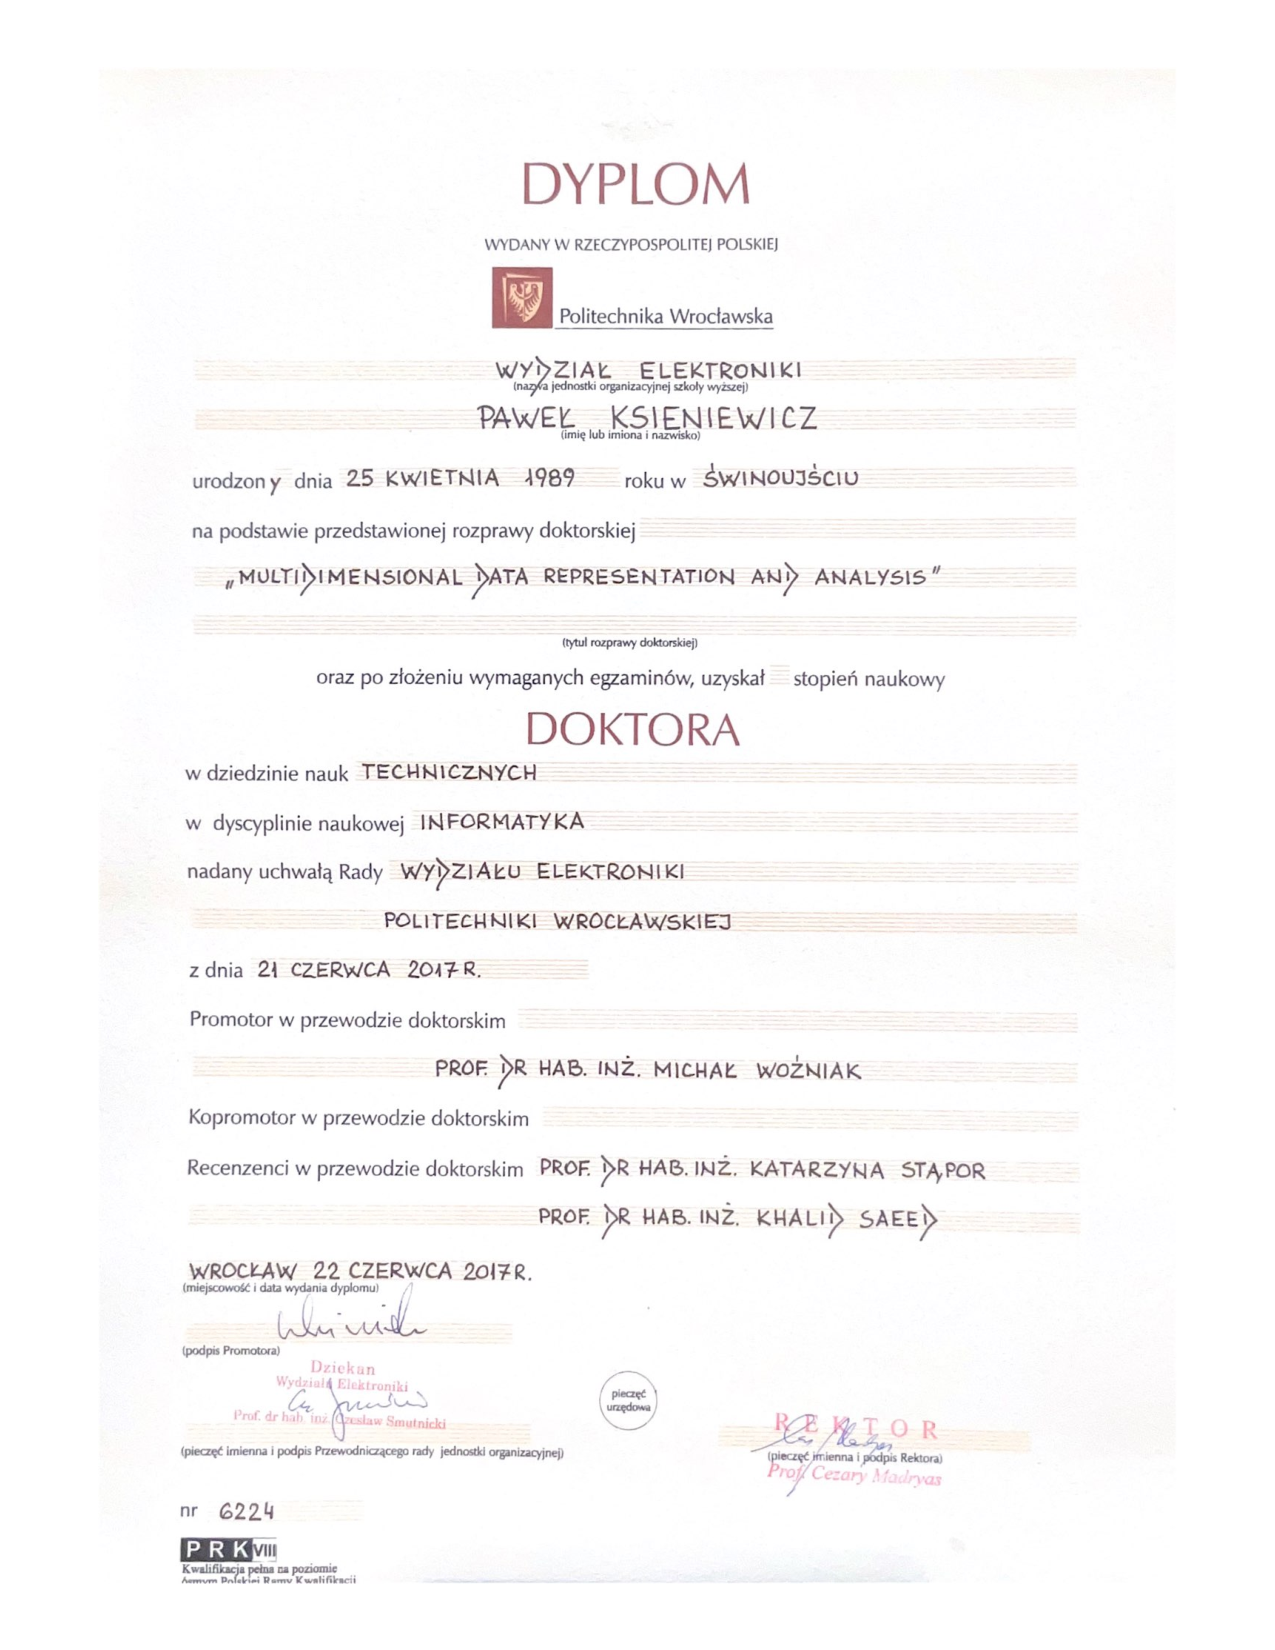
\includepdf[pages=-]{zal/DYPLOM.pdf}

\thispagestyle{empty}
%\cleardoublepage
\begin{fullwidth}
\chapter{Autoreferat wnioskodawcy}

	\section{Imię i nazwisko}

\vspace{-.5em}Paweł Ksieniewicz\vspace{-1em}

\section{Posiadane dyplomy, stopnie naukowe lub artystyczne -- z podaniem podmiotu nadającego stopień, roku ich uzyskania oraz tytułu rozprawy doktorskiej}

\vspace{-.5em}\begin{tabular}{lrp{25em}}
\textbf{\oldstylenums{2017}} & 	\multicolumn{2}{p{30em}}{\textbf{Stopień doktora nauk technicznych w dyscyplinie Informatyka.}}\\
&\multicolumn{2}{l}{\emph{Nadany uchwałą Rady Wydziału Elektroniki Politechniki Wrocławskiej.}}\\\\
&Tytuł rozprawy: & \emph{Multidimensional data representation and analysis}\\
&Tytuł w języku polskim:&\emph{Reprezentacja i analiza danych wielowymiarowych}\\
&Promotor: &\emph{prof. dr hab. inż. Michał Woźniak}\\\\

\textbf{\oldstylenums{2017}} & 	\multicolumn{2}{p{30em}}{\textbf{Tytuł zawodowy magistra inżyniera w dyscyplinie Informatyka.}}\\
&\multicolumn{2}{l}{\emph{Wydział Elektroniki Politechniki Wrocławskiej.}}\\\\
&Tytuł pracy magisterskiej: & \emph{System wykrywania sztormów na Morzu Bałtyckim z wykorzystaniem metorogramów}\\
&Promotorka: &\emph{dr inż. Iwona Poźniak-Koszałka}\\\\
\end{tabular}\vspace{-1em}

\section{Informacje o dotychczasowym zatrudnieniu w jednostkach naukowych lub artystycznych}

\vspace{-.5em}\begin{tabular}{r@{}c@{}lp{40em}}
\bfseries 10.2017 & \bfseries~--~ & \bfseries obecnie & \textbf{Adiunkt}\\

&&& Katedra Systemów i Sieci Komputerowych\\
&&& Wydział Informatyki i Telekomunikacji\\
&&& Politechnika Wrocławska\\
&&& \emph{(do roku 2021 w Katedrze Systemów i Sieci Komputerowych Wydziału Elektroniki PWr)}\\\\

\bfseries 5.2019 & \bfseries~--~ & \bfseries 11.2021 & \textbf{Specjalista ds. sztucznej inteligencji}}\\

&&& Uniwersytet Technologiczno-Przyrodniczy im. Jana i Jędrzeja Śniadeckich w Bydgoszczy\\\\
%&&& Wydział Elektroniki\\
%&&& Politechnika Wrocławska\\

\bfseries 2.2015 & \bfseries~--~ & \bfseries 10.2017 & \textbf{Asystent}\\

&&& Katedra Systemów i Sieci Komputerowych\\
&&& Wydział Elektroniki\\
&&& Politechnika Wrocławska\\

\end{tabular}\vspace{-1em}


%\newpage

% 3.4
\section{Omówienie osiągnięć, o których mowa w art. 219 ust. 1 pkt. 2 ustawy z dnia 20 lipca 2018 r. Prawo o szkolnictwie wyższym i nauce (Dz. U. z 2021 r. poz. 478 z późn. zm.)}

	
	\subsection{Tytuł osiągnięcia naukowego}
W ramach niniejszego wniosku habilitacyjnego prezentowane jest osiągnięcie w formie cyklu powiązanych ze sobą tematycznie publikacji pod zbiorczym tytułem:

%\begin{fullwidth}
\vspace{1em}
\begin{center}
	\LARGE
	\textbf{Projektowanie algorytmów rozpoznawania wzorców dla~zadania klasyfikacji trudnych danych}
\end{center}\vspace{1em}
%\end{fullwidth}


\end{fullwidth}

\begin{fullwidth}
\subsection{Wykaz publikacji wchodzących w skład cyklu}


Zamieszczony poniżej ciąg publikacji ułożony jest w odwrotnej kolejności chronologicznej, stanowiąc listę jedenastu artykułów opublikowanych w latach 2017--2022. Wszystkie podane przy nich wartości bibliometryczne oddają \textbf{stan na dzień 27. sierpnia 2022 r.} zgodnie z bazami publikacji naukowych:
\end{fullwidth}

\begin{itemize}
	\item[\textsc{WoS}] \emph{Web of Science}%\marginnote[0em]{\noindent
\includegraphics[width=1.5cm]{WoS.png}}
	%\begin{flushright}
	
	\url{https://www.webofscience.com/wos/author/record/1886494}	
	%\end{flushright}
	
	\item[\textsc{Sco}] \emph{Scopus}%\marginnote[0em]{\noindent
\includegraphics[width=1.5cm]{Scopus.png}}
	%\begin{flushright}
	
	\url{https://www.scopus.com/authid/detail.uri?authorId=56206176100}
	%\end{flushright}
	
	\item[\textsc{GSc}] \emph{Google Scholar}%\marginnote[0em]{\noindent
\includegraphics[width=1.5cm]{GSc.png}}
	%\begin{flushright}
	
	\url{https://scholar.google.com/citations?user=YSM30D8AAAAJ}
	%\end{flushright}\vspace{1em}
	\vfill
	
	\item Wpisy bibliograficzne dla artykułów w czasopismach zostały uzupełnione o~informację o wartości czynnika \emph{Impact Factor}\sidenote[][-1em]{Journal Citation Reports --- \url{https://clarivate.com/webofsciencegroup/solutions/journal-citation-reports}} wydawnictwa z~roku publikacji.
	\item Dla artykułów konferencyjnych podano informację o~poziomie konferencji według rankingu \textsc{core}\footnote{CORE Rankings Portal --- \url{https://www.core.edu.au/conference-portal}} w~roku publikacji. 
	\item Każdy wpis zawiera także informację o~liczbie punktów \emph{Ministerstwa Edukacji i Nauki} (\textsc{me}i\textsc{n}) w roku publikacji.
	\item Do każdej pozycji ze spisu publikacji wchodzących w skład cyklu została dodana również informacja o moim wkładzie autorskim, zgodnie z wytycznymi wzorca \textsc{CRediT} (\emph{Contributor Roles Taxonomy})\sidenote[][-3em]{\textsc{CRediT} author statement -- \url{https://www.elsevier.com/authors/policies-and-guidelines/credit-author-statement}}. Określenia te pokrywają się z deklaracjami współautorów zawartymi w Załączniku 5 do wniosku.
\end{itemize}
\vfill
\newpage

%
% C1
%
\marginnote[1em]{
% MARGIN TAB
\color{red}
\begin{tabular}{rccc}
\toprule
& \textsc{WoS} & \textsc{Sco} & \textsc{GSc}\\
l. cytowań & --- & --- & --- \\\\
\multicolumn{3}{r}{\color{black}\emph{Szacowany udział}} & \color{black}70\%\\
\multicolumn{3}{r}{\color{black}\emph{Impact Factor}} & \color{black}8.139\\
\multicolumn{3}{r}{\color{black}\emph{l. punktów \textsc{me}i\textsc{n}}} & \color{black}200\\\\

%\multicolumn{4}{r}{
\includegraphics[width=1.5cm]{WoS.png}}
\end{tabular}

% BASE TAB
}\noindent\begin{tabular}{lllll@{}}
\toprule
\color{red}[C1] & \multicolumn{4}{p{28em}}{\fullcite{C1}} \\
 & \multicolumn{4}{p{30em}}{
 {\footnotesize\textsc{CRediT}}: 
 \mybox{Conceptualization} \mybox{Software} \mybox{Validation} \mybox{Investigation} \mybox{Writing - Original Draft} \mybox{Writing - Review \& Editing} \mybox{Visualization} \mybox{Supervision}}\\

%\\\\\bottomrule
\end{tabular}
\vspace{.5em}

%
% C2
%
\marginnote[1em]{
% MARGIN TAB
\color{red}
\begin{tabular}{rccc}
\toprule
& \textsc{WoS} & \textsc{Sco} & \textsc{GSc}\\
l. cytowań & --- & --- & --- \\\\
\multicolumn{3}{r}{\color{black}\emph{Szacowany udział}} & \color{black}100\%\\
\multicolumn{3}{r}{\color{black}\emph{Impact Factor}} & \color{black}5.086\\
\multicolumn{3}{r}{\color{black}\emph{l. punktów \textsc{me}i\textsc{n}}} & \color{black} 70\\\\

%\multicolumn{4}{r}{
\includegraphics[width=1.5cm]{WoS.png}}

\end{tabular}
% BASE TAB
}\noindent\begin{tabular}{lllll@{}}
\toprule
\color{red}[C2] & \multicolumn{4}{p{28em}}{\fullcite{C2}}  \\
 & \multicolumn{4}{p{30em}}{
 {\footnotesize\textsc{CRediT}}: 
 \mybox{Conceptualization} \mybox{Methodology} \mybox{Software} \mybox{Validation} \mybox{Formal Analysis} \mybox{Investigation} \mybox{Resources} \mybox{Data Curation} \mybox{Writing - Original Draft} \mybox{Writing - Review \& Editing} \mybox{Visualization}}\\
%\\\\\bottomrule
\end{tabular}
\vspace{2.5em}

%
% C3
%
\marginnote[1em]{
% MARGIN TAB
\color{red}
\begin{tabular}{rccc}
\toprule
& \textsc{WoS} & \textsc{Sco} & \textsc{GSc}\\
l. cytowań & 2 & 1 & 4 \\\\
\multicolumn{3}{r}{\color{black}\emph{Szacowany udział}} & \color{black}70\%\\
\multicolumn{3}{r}{\color{black}\emph{Core}} & \color{black}B\\
\multicolumn{3}{r}{\color{black}\emph{l. punktów \textsc{me}i\textsc{n}}} & \color{black} 140\\\\

%\multicolumn{4}{r}{
\includegraphics[width=1.5cm]{WoS.png}}

\end{tabular}
% BASE TAB
}\noindent\begin{tabular}{lllll@{}}
\toprule
\color{red}[C3] & \multicolumn{4}{p{28em}}{\fullcite{C3}}  \\
 & \multicolumn{4}{p{30em}}{
 {\footnotesize\textsc{CRediT}}: 
 \mybox{Conceptualization} \mybox{Validation} \mybox{Formal Analysis} \mybox{Investigation} \mybox{Resources} \mybox{Writing - Original Draft} \mybox{Writing - Review \& Editing} \mybox{Visualization} \mybox{Supervision}}\\

%\\\\\bottomrule
\end{tabular}
\vspace{.5em}

%
% C4
%
\marginnote[1em]{
% MARGIN TAB
\color{red}
\begin{tabular}{rccc}
\toprule
& \textsc{WoS} & \textsc{Sco} & \textsc{GSc}\\
l. cytowań & 2 & 2 & 4 \\\\
\multicolumn{3}{r}{\color{black}\emph{Szacowany udział}} & \color{black}100\%\\
\multicolumn{3}{r}{\color{black}\emph{Impact Factor}} & \color{black}5.719\\
\multicolumn{3}{r}{\color{black}\emph{l. punktów \textsc{me}i\textsc{n}}} & \color{black} 140\\\\

%\multicolumn{4}{r}{
\includegraphics[width=1.5cm]{WoS.png}}

\end{tabular}

% BASE TAB
}\noindent\begin{tabular}{lllll@{}}
\toprule
\color{red}[C4] & \multicolumn{4}{p{28em}}{\fullcite{C4}}  \\
 & \multicolumn{4}{p{30em}}{
 {\footnotesize\textsc{CRediT}}: 
 \mybox{Conceptualization} \mybox{Methodology} \mybox{Software} \mybox{Validation} \mybox{Formal Analysis} \mybox{Investigation} \mybox{Resources} \mybox{Data Curation} \mybox{Writing - Original Draft} \mybox{Writing - Review \& Editing} \mybox{Visualization}}\\

%\\\\\bottomrule
\end{tabular}
\vspace{2.5em}
%\newpage

%
% C5
%
\marginnote[1em]{
% MARGIN TAB
\color{red}
\begin{tabular}{rccc}
\toprule
& \textsc{WoS} & \textsc{Sco} & \textsc{GSc}\\
l. cytowań & 6 & 7 & 13 \\\\
\multicolumn{3}{r}{\color{black}\emph{Szacowany udział}} & \color{black}50\%\\
\multicolumn{3}{r}{\color{black}\emph{Core}} & \color{black}A\\
\multicolumn{3}{r}{\color{black}\emph{l. punktów \textsc{me}i\textsc{n}}} & \color{black} 140\\\\

%\multicolumn{4}{r}{
\includegraphics[width=1.5cm]{WoS.png}}
\end{tabular}

% BASE TAB
}\noindent\begin{tabular}{lllll@{}}
\toprule
%\color{red}[C5] & \multicolumn{4}{p{28em}}{\fullcite{C5}}  \\
\color{red}[C5] & \multicolumn{4}{p{28em}}{Paweł Ksieniewicz, Paweł Zyblewski, Michał Choraś, Rafał Kozik, Agata Giełczyk, Michał Woźniak, \emph{"Fake News Detection from Data Streams"}. W: \emph{2020 International Joint Conference on Neural Networks (IJCNN)}. 2020, s. 1-8. \textsc{doi}: \verb|\url{10.1109/IJCNN48605.2020.9207498}}  \\
 & \multicolumn{4}{p{30em}}{
 {\footnotesize\textsc{CRediT}}: 
 \mybox{Conceptualization} \mybox{Methodology} \mybox{Software} \mybox{Validation} \mybox{Investigation} \mybox{Writing - Original Draft} \mybox{Writing - Review \& Editing} \mybox{Visualization}}\\

%\\\\\bottomrule
\end{tabular}
\newpage

%
% C6
%
\marginnote[1em]{
% MARGIN TAB
\color{red}
\begin{tabular}{rccc}
\toprule
& \textsc{WoS} & \textsc{Sco} & \textsc{GSc}\\
l. cytowań & 4 & 5 & 5 \\\\
\multicolumn{3}{r}{\color{black}\emph{Szacowany udział}} & \color{black}100\%\\
\multicolumn{3}{r}{\color{black}\emph{Core}} & \color{black}C\\
\multicolumn{3}{r}{\color{black}\emph{l. punktów \textsc{me}i\textsc{n}}} & \color{black} 20\\\\

%\multicolumn{4}{r}{
\includegraphics[width=1.5cm]{WoS.png}}

\end{tabular}

% BASE TAB
}\noindent\begin{tabular}{lllll@{}}
\toprule
\color{red}[C6] & \multicolumn{4}{p{28em}}{\fullcite{C6}}  \\
 & \multicolumn{4}{p{30em}}{
 {\footnotesize\textsc{CRediT}}: 
 \mybox{Conceptualization} \mybox{Methodology} \mybox{Software} \mybox{Validation} \mybox{Formal Analysis} \mybox{Investigation} \mybox{Resources} \mybox{Data Curation} \mybox{Writing - Original Draft} \mybox{Writing - Review \& Editing} \mybox{Visualization}}\\

%\\\\\bottomrule
\end{tabular}
\vspace{2.5em}

%
% C7
%
\marginnote[1em]{
% MARGIN TAB
\color{red}
\begin{tabular}{rccc}
\toprule
& \textsc{WoS} & \textsc{Sco} & \textsc{GSc}\\
l. cytowań & 11 & 18 & 28 \\\\
\multicolumn{3}{r}{\color{black}\emph{Szacowany udział}} & \color{black}50\%\\
\multicolumn{3}{r}{\color{black}\emph{Impact Factor}} & \color{black}4.438\\
\multicolumn{3}{r}{\color{black}\emph{l. punktów \textsc{me}i\textsc{n}}} & \color{black} 140\\\\

%\multicolumn{4}{r}{
\includegraphics[width=1.5cm]{WoS.png}}

\end{tabular}
% BASE TAB
}\noindent\begin{tabular}{lllll@{}}
\toprule
%\color{red}[C7] & \multicolumn{4}{p{28em}}{\fullcite{C7}}  \\
\color{red}[C7] & \multicolumn{4}{p{28em}}{Paweł Ksieniewicz, Michał Woźniak, Bogusław Cyganek, Andrzej Kasprzak i Krzysztof Walkowiak. \emph{"Data stream classification using active learned neural networks"}. W: \emph{Neurocomputing 353 (2019)}, s. 74-82. \textsc{doi}: \verb|\url{10.1016/j.neucom.2018.05.130}}  \\
 & \multicolumn{4}{p{30em}}{
 {\footnotesize\textsc{CRediT}}: 
 \mybox{Methodology} \mybox{Software} \mybox{Validation} \mybox{Investigation} \mybox{Writing - Original Draft} \mybox{Writing - Review \& Editing} \mybox{Visualization}}\\

%\\\\\bottomrule
\end{tabular}
\vspace{2.5em}


%
% C8
%
\marginnote[1em]{
% MARGIN TAB
\color{red}
\begin{tabular}{rccc}
\toprule
& \textsc{WoS} & \textsc{Sco} & \textsc{GSc}\\
l. cytowań & --- & --- & 10 \\\\
\multicolumn{3}{r}{\color{black}\emph{Szacowany udział}} & \color{black}100\%\\
\multicolumn{3}{r}{\color{black}\emph{Core}} & \color{black}A\\
\multicolumn{3}{r}{\color{black}\emph{l. punktów \textsc{me}i\textsc{n}}} & \color{black} 140\\\\

%\multicolumn{4}{r}{
\includegraphics[width=1.5cm]{WoS.png}}

\end{tabular}
% BASE TAB
}\noindent\begin{tabular}{lllll@{}}
\toprule
\color{red}[C8] & \multicolumn{4}{p{28em}}{\fullcite{C8}}  \\
 & \multicolumn{4}{p{30em}}{
 {\footnotesize\textsc{CRediT}}: 
 \mybox{Conceptualization} \mybox{Methodology} \mybox{Software} \mybox{Validation} \mybox{Formal Analysis} \mybox{Investigation} \mybox{Resources} \mybox{Data Curation} \mybox{Writing - Original Draft} \mybox{Writing - Review \& Editing} \mybox{Visualization}}\\

%\\\\\bottomrule
\end{tabular}
\vspace{2.5em}

%
% C9
%
\marginnote[1em]{
% MARGIN TAB
\color{red}
\begin{tabular}{rccc}
\toprule
& \textsc{WoS} & \textsc{Sco} & \textsc{GSc}\\
l. cytowań & 6 & 11 & 13 \\\\
\multicolumn{3}{r}{\color{black}\emph{Szacowany udział}} & \color{black}80\%\\
\multicolumn{3}{r}{\color{black}\emph{Core}} & \color{black}B\\
\multicolumn{3}{r}{\color{black}\emph{l. punktów \textsc{me}i\textsc{n}}} & \color{black} 15\\\\

%\multicolumn{4}{r}{
\includegraphics[width=1.5cm]{WoS.png}}

\end{tabular}
% BASE TAB
}\noindent\begin{tabular}{lllll@{}}
\toprule
\color{red}[C9] & \multicolumn{4}{p{28em}}{\fullcite{C9}}  \\
 & \multicolumn{4}{p{30em}}{
 {\footnotesize\textsc{CRediT}}: 
 \mybox{Methodology} \mybox{Software} \mybox{Validation} \mybox{Investigation} \mybox{Writing - Original Draft} \mybox{Writing - Review \& Editing} \mybox{Visualization}}\\

%\\\\\bottomrule
\end{tabular}
\newpage

%
% C10
%
\marginnote[1em]{
% MARGIN TAB
\color{red}
\begin{tabular}{rccc}
\toprule
& \textsc{WoS} & \textsc{Sco} & \textsc{GSc}\\
l. cytowań & 15 & 15 & 18 \\\\
\multicolumn{3}{r}{\color{black}\emph{Szacowany udział}} & \color{black}60\%\\
\multicolumn{3}{r}{\color{black}\emph{Impact Factor}} & \color{black}4.072\\
\multicolumn{3}{r}{\color{black}\emph{l. punktów \textsc{me}i\textsc{n}}} & \color{black} 30\\\\

%\multicolumn{4}{r}{
\includegraphics[width=1.5cm]{WoS.png}}

\end{tabular}
% BASE TAB
}\noindent\begin{tabular}{lllll@{}}
\toprule
\color{red}[C10] & \multicolumn{4}{p{28em}}{\fullcite{C10}}  \\
 & \multicolumn{4}{p{30em}}{
 {\footnotesize\textsc{CRediT}}: 
 \mybox{Conceptualization} \mybox{Methodology} \mybox{Software} \mybox{Validation} \mybox{Writing - Original Draft} \mybox{Writing - Review \& Editing} \mybox{Visualization}}\\

%\\\\\bottomrule
\end{tabular}
\vspace{.5em}

%
% C11
%
\marginnote[1em]{
% MARGIN TAB
\color{red}
\begin{tabular}{rccc}
\toprule
& \textsc{WoS} & \textsc{Sco} & \textsc{GSc}\\
l. cytowań & --- & --- & 9 \\\\
\multicolumn{3}{r}{\color{black}\emph{Szacowany udział}} & \color{black}80\%\\
\multicolumn{3}{r}{\color{black}\emph{Core}} & \color{black}A\\
\multicolumn{3}{r}{\color{black}\emph{l. punktów \textsc{me}i\textsc{n}}} & \color{black} 140\\\\

%\multicolumn{4}{r}{
\includegraphics[width=1.5cm]{WoS.png}}

\end{tabular}
% BASE TAB
}\noindent\begin{tabular}{lllll@{}}
\toprule
\color{red}[C11] & \multicolumn{4}{p{28em}}{\fullcite{C11}}  \\
 & \multicolumn{4}{p{30em}}{
 {\footnotesize\textsc{CRediT}}: 
 \mybox{Conceptualization} \mybox{Methodology} \mybox{Software} \mybox{Validation} \mybox{Formal Analysis} \mybox{Investigation} \mybox{Resources} \mybox{Data Curation} \mybox{Writing - Original Draft} \mybox{Writing - Review \& Editing} \mybox{Visualization}}\\

\end{tabular}


\vfill

\subsection{Informacje naukometryczne}
Podane poniżej wartości oddają \textbf{stan na dzień 27. sierpnia 2022 r.} zgodnie z bazami publikacji naukowych \emph{Web of Science} (\textsc{WoS}), \emph{Scopus} (\textsc{Sco}) oraz \emph{Google Scholar} (\textsc{GSc}).

\vspace{4em}
\renewcommand{\arraystretch}{1.1}
\noindent\begin{tabular}{p{.9em}llrrr}
%\toprule
$\circ$ & \multicolumn{4}{l}{Sumaryczny IF dla osiągnięcia} & \multicolumn{1}{r}{27,454}\\

$\circ$ & \multicolumn{2}{l}{Sumaryczne MEiN} & & & \multicolumn{1}{r}{1~175}\\\\

& & & \textsc{\emph{WoS}} & \textsc{Sco} & \textsc{GSc}\\

$\circ$ & \multicolumn{2}{l}{Sumaryczna liczba cytowań dla osiągnięcia} & 46 & 59 & 104\\
$\circ$ & \multicolumn{2}{l}{Indeks Hirscha autora} & 8 & 10 & 13\\
 & & \multicolumn{1}{r}{\emph{l. cytowań.}} & 157 & 276 & 377\\
 & & \multicolumn{1}{r}{\emph{bez autocytowań}} & 134 & 240 & ---\\
 & & \multicolumn{1}{r}{\emph{l. dokumentów}} & 36 & 42 & 51\\
\end{tabular}


\vfill

\newpage
%\vspace{2em}
\section{Omówienie celu naukowego wyżej wymienionych prac, osiągniętych wyników oraz ich ewentualnego wykorzystania}\vspace{-1em}
Duży odsetek publikacji w tematyce systemów nadzorowanego uczenia się maszyn rozpoczynany jest parafrazą zdania \emph{"współczesny świat wypełniony jest danymi"}. Przyczynia się do tego wiele postępujących czynników, rozpoczynając od tak pozytywnych zjawisk jak masowa digitalizacja treści\citeZ[-5.5em]{Z1}, automatyzacja procesów produkcyjnych\citeZ[-1em]{Z2} czy rosnąca rola  systemów rekomendacyjnych~\citeZ[.5em]{Z3}. 

Należy jednak zwrócić również uwagę na bardziej złożone społecznie zjawiska takie jak popularyzacja wykorzystania pojazdów autonomicznych, w tym w usługach kurierskich i transportowych redukujących czynnik ludzki\citeZ[.5em]{Z4}, spadająca jakość produktów elektronicznych powodująca zwiększoną potrzebę automatycznych systemów diagnostyki sprzętu\citeZ[.5em]{Z5}, modelowanie zachowań ludzkich i -- szczególnie niepokojące -- profilowanie konsumentów w świecie, w którym dominująca większość naszych zachowań pozostawia swój ślad cyfrowy\citeZ[.5em]{Z6}. Proces ten wzmacniany jest także przez trwającą nieprzerwanie od końca \oldstylenums{2019} roku pandemię wirusa \emph{SARS-CoV-2}, który w dniu finalnej redakcji tego dokumentu dotknął bezpośrednio już ponad pół miliarda mieszkańców Ziemi, stanowiąc dodatkowy, niezaprzeczalny argument za automatyzacją czynności i procedur, które dotychczas wykonywane były przez odpowiednio wyszkolonych do tego celu ludzi.

Już w latach siedemdziesiątych zauważone zostało, zarówno w krytycznym dla całego środowiska maszyn uczących się raporcie Lighthilla\citeZ{Z7}, jak i w merytorycznych ocenach ówczesnego stanu badań nad systemami sztucznej inteligencji\citeZ[.5em]{Z8}, że indukcyjne modele predykcyjne najlepiej radzą sobie z problemami opisywanymi przez stosunkowo niewielką liczbę atrybutów. Przy silnie ograniczonej mocy obliczeniowej komputerów tamtej epoki\citeZ[.5em]{Z9}, większość publikacji opierała zawarte w nich obserwacje na temat efektywności poszczególnych metod rozpoznawania na tzw. \emph{toysetach} (zbiorach ilustracyjnych), ograniczonych do zaledwie kilku wymiarów i opisanych przez nie więcej niż kilkaset instancji. Ograniczenia te istotnie utrudniały generalizację wniosków na problemy rzeczywiste, opisywane przez potencjalnie nieskończone zbiory danych o wysokiej liczbie atrybutów.

Metody uczenia nadzorowanego, zgodnie z powszechnie przyjętą taksonomią, skupiają się na zadaniach regresji i klasyfikacji\citeZ{Z10}. W~pierwszym z tych przypadków rolą systemu rozpoznawania jest zyskanie zdolności do wyznaczania, najczęściej ciągłej, wartości zmiennej objaśnianej na podstawie zbioru odpowiednio anotowanych obserwacji. W~zadaniu klasyfikacji -- na którym skupia się większość prowadzonych przeze mnie badań -- obiekty przypisywane są do jednej z predefiniowanych kategorii nazywanych klasami problemu. W wypadku rzeczywistych zbiorów danych dla zadania klasyfikacji stosunkowo rzadka jest sytuacja, w której dysponujemy równomierną reprezentacją każdej z tych kategorii, co przynosi dodatkową trudność w ich analizie\citeZ[-7em]{Z11}. Trudność ta jest na tyle silna, że pozwoliła na wyodrębnienie się istotnego nurtu badań nad klasyfikacją danych niezbalansowanych\citeZ[-4.5em]{Z12}.

Modele klasyfikacji, często niezależnie od rodziny z której pochodzą, wykazują silną tendencję do faworyzowania decyzji w kierunku klasy dominującej zbiór danych\citeZ[-1.5em]{Z13}. Przykładowo, reguły splitu drzew decyzyjnych, przypisując etykietę do wierzchołka budowanego grafu uwzględniają przede wszystkim proporcję pomiędzy etykietami zakreślonych jego parametrami obiektów\citeZ[-.5em]{Z14}. Funkcje straty wykorzystywane w trenowaniu sieci neuronowych najczęściej tym samym kosztem obciążają błędne decyzje względem każdej z klas problemu\citeZ[.5em]{Z15}. Wreszcie, proste podejścia do rozpoznawania takie jak klasyfikatory minimalnoodległościowe, również wykazują tendencję do premiowania obiektów klas o większym prawdopodobieństwie \emph{a priori}, co w każdym z wymienionych przypadków prowadzi do budowy modeli nadmiernie ograniczających obszar decyzyjny klasy mniejszościowej~\citeZ[-1em]{Zyb19}.

Najpowszechniej występujące współcześnie trudności przetwarzania danych powiązane są z czynnikiem ich masowości, dokładniej opisywanym przez model 4V Big Data\citeZ[.5em]{Z16}. Masowość danych wyrażać może się zarówno we wspomnianym już kontekście wielowymiarowości, jak też w niezwykle dużej liczności zbiorów. Pierwotną motywacją badań w tym zakresie były ograniczenia obliczeniowe i pamięciowe maszyn z drugiej połowy \textsc{xx} wieku, które nie pozwalały ani na jednoczesne składowanie pełnego zbioru danych, ani na przetworzenie wszystkich dostępnych wzorców w akceptowalnym czasie obliczeniowym\citeZ[-1em]{Z17}. Podstawowe rozwiązania w tym zakresie wprowadzają paradygmat tzw.~uczenia inkrementalnego, dostępny zarówno dla prostych modeli takich jak \emph{Naive Bayes} czy niektóre drzewa decyzyjne\citeZ[.5em]{Z18}, jak i dla złożonych procedur optymalizacyjnych, wśród których największy nacisk należałoby położyć na sieci neuronowe~\citeZ{Z19}.

Typowy przypadek uczenia inkrementalnego, podobnie jak bardziej ogólna koncepcja \emph{i. i. d.} (ang. \emph{independent and identically distributed}) stanowiąca kluczowe zagadnienie walidacji modeli rozpoznawania, opiera się na założeniu o stacjonarności koncepcji, tj. na niezmienności prawdopodobieństwa \emph{a~posteriori} problemu. Dzięki takiemu założeniu, algorytm uczenia pozwalający na aktualizację wiedzy otrzymuje w każdym kroku wsad z dostępnych danych uczących -- w zależności od zastosowanego podejścia rozłączny lub losowy -- i dokonuje korekty modelu na ich podstawie. Korekta ta uwzględnia fakt, że systemowi rozpoznawania dostarczone zostały już wcześniej pewne przykłady opisujące problem i z czasem rola nowych obiektów jest coraz mniejsza, pozwalając na konwergencję modelu~\citeZ{Z20}.

Dziedzina przetwarzania strumieni danych rozwija paradygmat uczenia inkrementalnego o uwzględnienie czynnika czasu przez uznanie zbioru obiektów za uporządkowaną sekwencję. Daje to zarówno podstawę do właściwego spojrzenia na prędkość przetwarzania danych -- ponieważ obserwacje opisywane są i w czasie i przestrzeni -- jak i rozszerzenie pojęcia różnorodności poza heterogeniczność źródeł, przez zniesienie założenia o stacjonarności koncepcji. Procedury uczenia w~takim środowisku muszą ulegać zmianie i nie dążyć już do analizy stabilnego zjawiska, ale do konsekwentnej modyfikacji założeń na jego temat, znajdujących odzwierciedlenie w modelu zdolnym do śledzenia dynamiki jego zmian~\citeZ[-3em]{Z21}. 

Zmiany tego rodzaju zwykło się w literaturze nazywać dryfami lub dryftami koncepcji (ang. \emph{concept drift})~\citeZ[-2em]{Z22}. W uproszczonej taksonomii możemy wyróżnić dryfy wirtualne -- zmieniające co prawda rozkład klas w przestrzeni, ale nie mające istotnego wpływu na zmiany we właściwej granicy decyzyjnej oraz dryfy rzeczywiste -- stanowiące podstawowe źródło czasowej degeneracji modeli i najczęściej spotykane w strumieniach rzeczywistych. Degeneracja modelu może być również tymczasowym spadkiem jego zdolności generalizacyjnej, w wypadku strumieni o koncepcjach nawracających (ang. \emph{recurrent drift}), typowych dla danych opisujących zjawiska okresowe o uporządkowanej (cykl dobowy, cykl roczny) lub nieuporządkowanej (pogoda, rynek giełdowy) naturze.

\vspace{-.5em}\noindent \newthought{Podział cyklu publikacji na obszary tematyczne}~\\
\noindent Od roku złożenia rozprawy doktorskiej, która podejmowała tematykę metod reprezentacji i klasyfikacji danych wielowymiarowych, w~swoich pracach badawczych stale rozwijam metody pozwalające na efektywne przetwarzanie danych obciążonych wymienionymi wyżej trudnościami. Biorąc je pod uwagę, do typowego dla wstępów do prac z dziedziny stwierdzenia o tym, że \emph{świat wypełniony jest danymi}, warto byłoby dodać informację, iż dane te -- tak samo jak świat, który opisują -- ulegają ciągłym zmianom, a efektywne systemy rozpoznawania powinny być zdolne do ich rejestrowania i nadążania za nimi.

W kolejnych sekcjach opiszę zaproponowane przeze mnie metody oraz towarzyszące im publikacje, wpisujące się w opisaną tematykę i~będące podstawą osiągnięcia naukowego. Listę jedenastu artykułów naukowych stanowiących opisywany cykl wpisałem w trzy przenikające się kategorie:

\begin{enumerate}
	\item[\emph{I}] Algorytmy przetwarzania danych wielowymiarowych.
	\item[\emph{II}] Algorytmy przetwarzania danych niezbalansowanych.
	\item[\emph{III}] Algorytmy przetwarzania strumieni danych.
\end{enumerate}

\begin{figure}[h]
	\centering
	\scalebox{.6}{\large
	\def\imbcircle{(-210:2) circle (2.725cm)}
	\def\dscircle{(-330:2) circle (2.725cm)}
	\def\mdcircle{(-90:2) circle (2.725cm)}

	\begin{tikzpicture}
		%\draw[step=1.0,black,thin,dotted] (-5,-5) grid (5,5);
      	\begin{scope} % W miarę
    		%\clip \firstcircle;
    		%\fill[green!25] \mdcircle;
      	\end{scope}
      	\begin{scope} % W miarę
    		%\clip \firstcircle;
    		%\fill[yellow!25] \imbcircle;
      	\end{scope}
      	\begin{scope} % Git
    		%\clip \firstcircle;
    		%\fill[green!25] \dscircle;
      	\end{scope}
      	\begin{scope} % Problematyczny
    		%\clip \dscircle;
    		%\fill[red!25] \mdcircle;
      	\end{scope}
      	
      	\node[fill=black,rotate=-210-90, text width=5.25cm, text height=2.9cm] at (-210:3.625) {};
      	\node[fill=black,rotate=-330-90, text width=5.25cm, text height=2.9cm] at (-330:3.625) {};
      	\node[fill=black,rotate=0, text width=5.25cm, text height=2.9cm] at (-90:3.625) {};
      	
      	\node[color=white,fill=black,rotate=-210-90,rounded corners=.25cm, text width=5.25cm, align=center] at (-210:5.25) {\bfseries \textsc{dane niezbalansowane}};
      	\node[color=white,fill=black,rotate=-330-90,rounded corners=.25cm, text width=5.25cm, align=center] at (-330:5.25) {\bfseries \textsc{strumienie danych}};
		\node[color=white,fill=black,rotate=0,rounded corners=.25cm, text width=5.25cm, align=center] at (-90:5.25) {\bfseries \textsc{dane wielowymiarowe}};


    	\draw[fill=white] \imbcircle;
      	\draw[fill=white] \dscircle;
      	\draw[fill=white] \mdcircle;

      	
    	\draw[ultra thick] \imbcircle;
      	\draw[ultra thick] \dscircle;
      	\draw[ultra thick] \mdcircle;
      	

      	%\node[fill=white,rotate=-210-90,rounded corners=.25cm, text width=3cm, align=center] at (-210:4.5) {\bfseries Dane\\Niezbalansowane};
      	%\node[fill=white,rotate=-330-90,rounded corners=.25cm] at (-330:4.5) {\bfseries DS};
      	%\node[fill=white,rotate=-90+90,rounded corners=.25cm] at (-90:4.5) {\bfseries MD};
      	
      	% IMB
      	\node at (-210:3) {[C6]}; %7
      	
      	% IMB + DS
      	\node at (90:1.75) {[C3]};
      	\node at (90:1.25) {[C4]}; % 6
      	
      	% DS
      	\node at (-330:2.5) {[C7]};
      	\node at (-330:3.5) {[C1]};
      	
      	% MD
      	\node at (-90:2.5) {[C11]}; % 11
      	\node at (-90:3.5) {[C10]}; % 15
    
    	% IMB + MD
      	\node at (-330-180:1.25) {[C9]}; % 14
      	\node at (-330-180:2) {[C8]}; % 19
      	%\node at (-330-180:2.25) {[C10]}; % 19  	
      	
      	% DS + MD
      	\node at (-210-180:1.25) {[C5]};
      	
      	% ALL
      	\node at (0:0) {[C2]};
	\end{tikzpicture}}
	\caption{Przypisanie prac z cyklu publikacji do zakresu tematycznego klasyfikacji danych trudnych. Podane w nawiastach kwadratowych indentyfikatory odwołują się do spisu zawartego w P4.}\label{fig:philips}
\end{figure}

Przypisanie poszczególnych prac do kategorii zostało zilustrowane w~Rysunku~\ref{fig:philips} zawierającym nachodzące na siebie obszary badawcze wraz ze stosownymi odniesieniami literaturowymi.

\subsection*{I -- Algorytmy przetwarzania danych wielowymiarowych}

\marginnote{\scalebox{.6}{\large
	\def\imbcircle{(-210:2) circle (2.725cm)}
	\def\dscircle{(-330:2) circle (2.725cm)}
	\def\mdcircle{(-90:2) circle (2.725cm)}

	\begin{tikzpicture}
      	
      	\node[fill=black,rotate=0, text width=5.25cm, text height=2.9cm] at (90:-.5) {};
		\node[color=white,fill=black,rotate=0,rounded corners=.25cm, text width=5.25cm, align=center] at (90:1.25) {\bfseries \textsc{dane wielowymiarowe}};
      	
      	\draw[fill=white] \mdcircle;
      	\draw[ultra thick] \mdcircle;
      	
      	% 10 9 11 
      	% MD
      	\node at (-90:.5) {[C11]};
      	\node at (-90:1.25) {[C10]};    
      	\node at (-90:2.0) {[C9]};
      	%\node at (-330-180:1.75) {[4]};
      	      	   
      	\node at (-90:2.75) {\color{black!50}\emph{[C8]}};   
      	\node at (-90:3.5) {\color{black!50}\emph{[C2]}};
      	% DS + MD
      	%\node at (-210-180:1.25) {[5]};
      	%\node at (-210-180:1.75) {[6]};
      	
      	% ALL
      	%\node at (0:0) {[7]};
	\end{tikzpicture}}}

Po prawej stronie diagram zaznaczający opisywane w ramach wątku przetwarzania danych wielowymiarowych, wliczający prace opisane w~innych wątkach dominujących.

Najsilniej rozwijającą się w ostatnim dziesięcioleciu odpowiedzią środowiska naukowego na stale rosnącą wymiarowość danych jest bez wątpienia nurt uczenia reprezentacji (ang. \emph{representation learning}). Dedykowany jest on głównie wielowymiarowym danym sygnałowym, w których najczęściej spotykamy bardzo silne, ale jednocześnie zmienne, relacje pomiędzy atrybutami, stanowiącymi najczęściej wartości poszczególnych elementów obrazu.

Niemniej jednak, nadal interesującą alternatywą są tutaj metody klasyczne, uwzględniające element manualnej inżynierii cech. Pozwalają one na wstępną redukcję atrybutów, które łatwiej jest opisać przez podprzestrzenną dywersyfikację nowej przestrzeni, konstruując tak już dwupoziomowy system rozpoznawania zdolny do budowy złożonych granic decyzyjnych nawet przy użyciu prostych klasyfikatorów bazowych.

Szczególnym przypadkiem obrazów cyfrowych są \emph{obrazy nadwidmowe}\footnote{W j. polskim brak jest powszechnie uznanej taksonomii dla danych o~ciągłym wymiarze spektralnym, w~związku z~czym posługuję się tutaj tłumaczeniem wykorzystywanym w~raportach sprawozdawczych, zaproponowanym w 2014 roku.} (ang. \emph{hyperspectral images}). Stanowią one efekt próbkowania promieniowania elektromagnetycznego zarówno w dwóch wymiarach przestrzennych -- jak standardowe obrazy -- jak i w wymiarze spektralnym, dzięki zastosowaniu pryzmatu rozszczepiającego promieniowanie elektromagnetyczne na wąskie, rozłączne pasma opisujące zakres częstotliwości przekraczający zdolność widzenia ludzkiego\footnote{Na przykładzie sensora \textsc{aviris}.}. W sytuacji, w której liczba takich pasm przekracza setkę, zbiór atrybutów dla każdego piksela przestaje być pulą luźno powiązanych ze sobą czynników (jak w reprezentacji \textsc{rgb} czy obrazach wielowidmowych) i staje się już typową dla obrazu nadwidmowego sygnaturą spektralną.

Stanowi to niezwykle interesujący przypadek danych rzeczywistych, w~których możemy mówić o ciągłości informacji w~każdym z~wymiarów obrazu. Sygnatura spektralna, którą najczęściej wykorzystujemy~w badaniach jako bazową reprezentację wzorca, jest jednowymiarowym sygnałem cyfrowym zbliżonym w~swoim przebiegu do wyraźnie zaszumionego wykresu funkcji wielomianowej. Szum ten najczęściej ma charakter globalny w~skali obrazu i typowy dla wykorzystanego sensora.

Dane nadwidmowe reprezentowane są przez tzw. \emph{kostki hiperspektralne} (ang. \emph{hyperspectral cubes}) będące trójwymiarowymi tensorami, które dla zadania klasyfikacji uzupełnione są o dwuwymiarową, dyskretną mapę \emph{ground truth}, tj. etykiet każdego piksela. Prezentują one najczęściej zdjęcia lotnicze pól uprawnych i~miast, budując wieloklasowe problemy niezbalansowane, choć zakres ich zastosowań wykracza też poza tę specyfikę i~odnajduje się -- przykładowo -- w obrazowaniu palimpsestów i~kontroli jakości produkcji.\vspace{1em}

{
\color{red}
\noindent\begin{tabular}{p{\textwidth}}
	\toprule &
\end{tabular}\vspace{-1em}
}
\noindent W \citeC[-2.25em]{C10} zaproponowałem autorską metodę budowy systemu rozpoznawania dla obrazów nadwidmowych, opartą o ręczną inżynierię atrybutów i zespołową integrację szybkich sieci neuronowych \emph{Extreme Learning Machines} (\textsc{elm}).

Silna zależność pomiędzy cechami zawartymi w~sygnaturze spektralnej powiązana jest z~równie silną nadmiarowością zapisanej w~niej informacji. Strategią przeciwdziałającą redundancji jest zerwanie ciągłości widmowej danych, którą możemy uzyskać przez selekcję atrybutów lub ich ekstrakcję. W selekcji jest to często operacja silnie stratna i~wzmacniająca rolę szumu w~pojedynczej próbce, a~w~ekstrakcji i~uczeniu reprezentacji -- gubiąca interpretowalność atrybutów. Alternatywą jest tutaj, wzorowana na właściwościach fotoreceptorów, ręczna inżynieria atrybutów, gdzie każda nowa cecha stanowi liniową kombinację elementów sygnatury bazowej, posiada swoją semantyczną interpretację i~wykazuje obniżoną zależność od pozostałych.

Zaproponowałem tu czternaście metryk statystycznych rozpinających się od prostych miar, takich jak minimum, średnia czy mediana sygnatury, przez metryki zróżnicowania sygnału reflektancji, interpretowanego jako zmienna losowa po pseudo kanały barwne uzyskane z projekcji całego obrazu do modelu \textsc{hsv}.

Należy mieć tu na uwadze, że inżynieria atrybutów oparta na miarach statystycznych jest nadal silnie czuła na błędy pomiarów, które są szczególnie widoczne w rzeczywistych obrazach nadwidmowych. Do~przeciwdziałania ich negatywnym skutkom wykorzystałem, zaproponowany przeze mnie w jednej z wcześniejszych prac, \emph{Entropodynamiczny Filtr Percentylowy}~\citeM{Ksi18e}, który pozwala na detekcję impulsywnych zmian sygnału i tym samym oznaczenie pasm sygnatury obciążonych wysokim błędem -- zakłócającym wartości metryk statystycznych.

Kluczowym zagadnieniem pracy było odpowiednie wykorzystanie potencjału algorytmu \textsc{elm}. Jego model neuronowy jest silnie oparty na losowości, pozwalając na~znacznie krótszy proces uczenia niż \textsc{mlp}, jednak kosztem znacznie wyższej wariancji modelu. Stabilizacja takiego rozwiązania często realizowana jest przez wykorzystanie uczenia zespołowego (ang. \emph{ensemble learning}), czego skuteczność została już potwierdzona w~wielu publikacjach~\citeZ[-3em]{Z23}. Krytyczny dla zespołu aspekt dywersyfikacji jego puli najczęściej opiera się na~losowości wag wejściowych, co~przy szerokim i silnie zależnym wewnętrznie wektorze atrybutów zdecydowanie nie jest rozwiązaniem optymalnym. Literatura pokazuje, że~dla danych tego typu znacznie lepszą strategią jest dywersyfikacja projekcyjna~\citeZ[-4.5em]{Z24} lub podprzestrzenna~\citeM[.5em]{Sul21}, która możliwa jest~do efektywnego zastosowania -- przykładowo -- po zaproponowanej ręcznej inżynierii cech. 

W wypadku dywersyfikacji podprzestrzennej (ang. \emph{random subspace}) musimy pamiętać o~zapewnieniu pełnego pokrycia oryginalnej przestrzeni atrybutów. Prawdopodobieństwo pokrycia możemy wyliczyć przez wzór:

\begin{equation}
	P(coverage) = 1 - (1-\frac{r}{d})^L,
\end{equation}

\noindent gdzie $r$ to wielkość podprzestrzeni, $d$ -- liczba atrybutów, a $L$ to wielkość puli. Naturalnie, przy zachowaniu stałej wielkości podprzestrzeni $r$, wraz ze wzrostem liczby wymiarów problemu powinniśmy też proporcjonalnie zwiększać pulę modeli, pamiętając jednak o tym, że po przekroczeniu pewnego limitu będzie ona wpływać negatywnie na różnorodność.

Przy wykorzystaniu 14. atrybutów statystycznych zamiast ponad 200. spektralnych\sidenote[]{Najczęściej wykorzystywany w danych benchmarkowych sensor \textsc{aviris} opisuje 224 pasma w widmie od 400 do 2 500 nanometrów.} możliwe jest więc zbudowanie mniejszego zespołu klasyfikatorów dywersyfikowanego przez \textsc{rsm} pozwalającego na pełne pokrycie przestrzeni atrybutów.

Zespoły \textsc{elm} domyślnie integruje się przez reguły głosowania większościowego, co daje duży potencjał do modyfikacji mających istotny wpływ na jakość docelowego modelu. W pracy proponuję więc komplementarnie ważoną integrację zespołu, gdzie za wyliczenie optymalnych wag -- dla każdej klasy indywidualnie -- odpowiada pojedynczy perceptron.

Uzyskane rezultaty badań pozwoliły na uprawdopodobnienie hipotezy stanowiącej o tym, że zespołowy model \textsc{elm} dywersyfikowany przez \textsc{rsm} z wykorzystaniem atrybutów statystycznych, integrowany z~wykorzystaniem wyuczalnej reguły decyzyjnej okazuje się statystycznie istotnie lepszy od podejść standardowych dla większości analizowanych zbiorów danych. Możemy dzięki nim zaobserwować też, że odpowiednia selekcja atrybutów, bez wykorzystywania metod wbudowanych czy resamplingu, może prowadzić do istotnego statystycznie ulepszenia modelu klasyfikacji nawet w wieloklasowych danych niezbalansowanych.\vspace{1em}

{
\color{red}
\noindent\begin{tabular}{p{\textwidth}}
	\toprule &
\end{tabular}\vspace{-1em}
}
\noindent Obserwacja ta stała się podstawą do badań przedstawionych w \citeC[-2.25em]{C9}. Stanowią one analizę odchodzącą już od specyfiki obrazów nadwidmowych, gdzie ewaluacja przeprowadzona została na kolekcji 35 tabelaryczych zbiorów o skali niezbalansowania sięgającej 1:41. 

Należy zaznaczyć, że punktem wyjściowym badań było wykorzystanie problemów o wstępnie zredukowanej wymiarowości -- przyjmując przestrzenie od 8 do 19 atrybutów -- i analiza potencjału metod optymalizacyjnych w selekcji podprzestrzeni do ulepszenia efektywności w~klasyfikacji niezbalansowanej.

W artykule zaproponowałem autorską metodę hybrydową wykorzystującą techniki selekcji atrybutów do budowy puli klasyfikatorów na potrzeby zespołu. Celem uniknięcia przeuczenia zastosowałem techniki regularyzacyjne zapewniające maksymalizację różnorodności zespołu przy jednocześniej minimalizacji wielkości podprzestrzeni dla każdego klasyfikatora bazowego. Zostały one wprowadzone do procedury optymalizacyjnej przez konstrukcję następującej funkcji kryterialnej:

\begin{equation}
	Q(\Pi) = BAC(\Pi)- \alpha * \frac{NF(\Pi)}{d}+ \beta * \frac{AH(\Pi)}{d},\label{eq:criterion1}
\end{equation}

\noindent gdzie $BAC(\Pi)$ wskazuje na zbalansowaną dokładność zespołu, którego pulę definiujemy jako $\Pi$, $d$ wskazuje na liczbę bazowych atrybutów problemu, a dalsze składowe definiują czynniki regularyzacyjne:

\begin{itemize}
	\item[$NF$] -- liczbę atrybutów dostępnych w puli, która podzielona przez $d$ daje skalę pokrycia oryginalnej przestrzeni problemu przez zespół -- sterowana przez hiperparametr $\alpha$.
	\item[$AH$] -- średnią odległość Hamminga pomiędzy słowami zakodowanymi jako binarne maski podprzestrzeni osobników -- sterowana przez hiperparametr $\beta$.
\end{itemize}

Szczególnie istotny wydaje się tutaj czynnik $AH$ stanowiący rodzaj metryki różnorodności, który w ustawieniu odwrotnej proporcjonalności do modułu atrybutów powinien pozwalać na eliminację klasyfikatorów o~wysokiej zależności statystycznej. 

Procedura optymalizacyjna rozpoczyna się od wygenerowania początkowej populacji puli klasyfikatorów

\begin{equation}
	Population = \{\Pi_1, \Pi_2, \ldots, \Pi_S\},
\end{equation}

\noindent gdzie parametr $S$, jako czynnik arbitralny, określa wielkość populacji. Jego zwiększanie wiąże się z wcześniejszą konwergencją optymalizacji, ale generuje też wykładniczy narzut obliczeniowy. Osobniki oceniane są przez kryterium określone w Równaniu~\ref{eq:criterion1}. Dla uproszczenia obliczeń algorytm stosuje prostą strategię przeszukiwania, w każdym kroku pozostawiając w puli jedynie najbardziej rokujący zespół, integrowany przez jedną z trzech zaproponowanych strategii:

\begin{itemize}
	\item[\textsc{r}] -- prosta akumulacja wsparć bez ważenia klasyfikatorów bazowych,
	\item[\textsc{w}] -- ważona akumulacja wsparć z wagami proporcjonalnymi do zbalansowanej dokładności osiąganej przez klasyfikatory bazowe,
	\item[\textsc{n}] -- ważona akumulacja wsparć z wagami stanowiącymi znormalizowaną zbalansowaną dokładność osiąganą przez klasyfikatory bazowe.
\end{itemize}

Otrzymane wyniki uprawdopodobniają hipotezę stanowiącą o tym, że selekcja atrybutów odgrywa krytyczną rolę w klasyfikacji danych niezbalansowanych. W większości przypadków zaproponowana przeze mnie metoda osiągała istotnie wyższe rezultaty niż modele wyuczone na pełnej dostępnej reprezentacji.
\vspace{1em}

{
\color{red}
\noindent\begin{tabular}{p{\textwidth}}
	\toprule &
\end{tabular}\vspace{-1em}
}
\noindent Warto zauważyć, że struktura tożsama logicznie z obrazami wielo- i~nadwidmowymi może zostać uznana za reprezentację nie tylko pojedynczego zdarzenia, ale i całej koncepcji. Praca \citeC[-5em]{C11} rozwija koncepcję takiej właśnie reprezentacji, nazywanej \emph{ekspozerem}.

Podstawowym założeniem ekspozera jest to, że wymiary przestrzenne dyskretnej reprezentacji sygnałowej mogą stanowić odwzorowanie planarnej projekcji problemu, a wymiar spektralny -- odpowiadać za niezależne próbkowanie go w klasach. Istotne zredukowanie jej rozdzielczości wraz z zaproponowaniem odpowiedniej reguły predykcyjnej pozwala na wykorzystanie jej jako efektywnego czasowo i jakościowo modelu rozpoznawania niepozostającego w silnej zależności z żadną wykorzystywaną powszechnie metodą indukcji. W wypadku ciągłego próbkowania wymiaru spektralnego stosowny model miałby potencjał do rozwiązywania zadania regresji, a przy podejściu dyskretnym -- możliwy byłby do zastosowania w zadaniu klasyfikacji.

Procedura budowy ekspozera inspirowana jest procesem naświetlania kliszy fotograficznej. Dlatego też, parametrami kontrolującymi indukcje są (a) ziarno filmu -- odpowiadające za gęstość próbkowania przestrzennego i (b) czynnik dyspersji światła -- odpowiedzialny za płynne złamanie zasady rozłączności kubełków histogramu. W przeciwieństwie do fizycznego pierwowzoru, struktura taka \emph{naświetlana} jest przez wiązkę wzorców zorganizowanych przestrzennie przez projekcję do dwuwymiarowej podprzestrzeni. Wynikiem takiej procedury jest nieskwantyzowany obraz cyfrowy, gdzie intensywność każdego punktu stanowi zakumulowaną gęstość rozkładu wzorców oddziałujących na jego sąsiedztwo.

\begin{figure}[!htb]
	\centering
	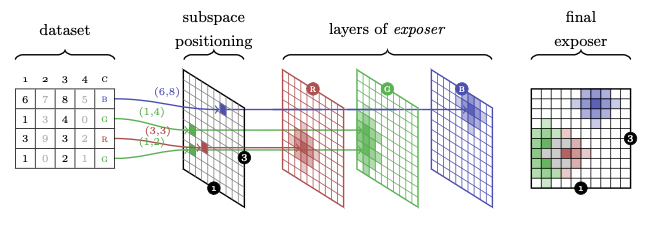
\includegraphics[width=\textwidth]{figures/exposer-projection}
	\caption{Ekspozycja czterech obiektów opisujących trzy klasy w dwuwymiarowej podprzestrzeni czterowymiarowego problemu.}\label{fig:exposer-projection}
\end{figure}

Wizualizacja procesu ekspozycji dla czterech obiektów opisujących trzy klasy w dwuwymiarowej podprzestrzeni czterowymiarowego problemu przedstawiona została na Rysunku~\ref{fig:exposer-projection}. W pierwszym kroku odbywa się tutaj pozycjonowanie podprzestrzenne, w którym każdy z obiektów zawartych w zbiorze uzyskuje nowe współrzędne w skończonej, planarnej projekcji na siatce $10\times 10$ (parametr ziarna). Ekspozer składa się z tylu warstw, ile klas zawiera się w zbiorze danych, a każda z~nich czuła jest jedynie na obiekty przynależącej do niej klasy.  

Przyjmijmy, że $\mathcal{DS}$ określa zbiór $n$ instancji, z których każda ($x_k$) reprezentowana jest przez $d$-wymiarowy wektor atrybutów oraz etykietę $i_k$ ze skończonego zbioru etykiet $\mathcal{M}$.

\begin{equation}
	\begin{array}[b]{llll}
		\mathcal{X} & \subseteq & \Re^d\\
		\mathcal{M}&=&\{1, 2, \ldots, M\}\\
		x_k & = & [x_k^{(1)}, x_k^{(2)}, \ldots, x_k^{(d)}]^{T}, & x_k \in \mathcal{X} \\
%		i_k & = & [i_1, i_2, \dots, i_n],                    & i_k \in \mathcal{M} \\
		\mathcal{DS} & = & \Big\{(x_1,i_1),(x_2,i_2),\ldots,(x_n,i_n)\Big\}
	\end{array}
\end{equation}

Różnorodność możliwych do zbudowania ekspozerów wyraża się przez zbiór $\Lambda$, zawierający ${d \choose s}$ kombinacji $\lambda_i$, gdzie $s$ stanowi wybraną wymiarowość ekspozera, w planarnym wypadku wynoszącą 2.

\begin{equation}
	\begin{array}[b]{llll}
		\Lambda   & = & \{\lambda_1, \lambda_2, \ldots, \lambda_L \}, & \vert\Lambda\vert = L= {d \choose s}                               \\
		\lambda_i & = & [l_1, l_2, \ldots, ,l_s],                     & l_j \in \{1, 2,\ldots, d\},\quad l_1\neq l_2 \neq \ldots \neq l_s,
	\end{array}
\end{equation}

Przy takich założeniach, reprezentacją ekspozera ($\mathcal{E}$) jest s-wymiarowa kostka danych:

\begin{equation}
	\begin{array}[b]{lll}
		\mathcal{E}_m & \in & G^s = \underbrace{G \times G \times \ldots \times G}_s                                                       \\
		\mathcal{E}   & =   & \{\mathcal{E}_1, \mathcal{E}_2, \ldots, \mathcal{E}_M \},
	\end{array}
\end{equation}

\noindent gdzie każda komórka adresowana przez $loc$ zawiera wektor wartości

\begin{equation}
	\begin{array}[b]{lll}
		\mathcal{E}^{(loc)} & = & [v_1, v_2, \ldots, v_M]^T       \\
		loc                 & = & [loc_1, loc_2, \ldots, loc_s]^T
	\end{array}
\end{equation}

Pojedyncza wartość jest sumą wszystkich pozytywnych różnic zadanego promienia oddziaływania $r$ z dystansem pomiędzy punktem centralnym komórki ($loc$) i każdym punktem $loc_k$ dla którego $i_k=m$. 

\vspace{-1em}\begin{equation}
	\begin{array}[b]{lll}
		\mathcal{E}_m^{(loc)} & = & \sum_{k=1}^{n}\Big[d(loc, loc_k) < r\;\wedge\; i_k = m\Big] \cdot \Big(r-d(loc,loc_k)\Big) \\
		loc_k                 & = & [ x_k^{(\lambda_1)}, x_k^{(\lambda_2)}, \ldots, x_k^{(\lambda_s)}]^T
	\end{array}
\end{equation}

Ekspozer $\mathcal{E}$, zbudowany na podprzestrzeni $\lambda$ zbioru uczącego $\mathcal{LS}$ może zostać wykorzystany do inferencji dla obiektu testowego $x_k$ ze zbioru testowego $\mathcal{TS}$ przez spróbkowanie go po projekcji do wspólnej przestrzeni

\begin{equation}
	\Psi(x_k) = \mathop{argmax}\limits_{m \in \mathcal{M}}\Big(\mathcal{E}^{(loc_k)}_m \Big).
\end{equation}

Podobnie jak w przypadku zastosowania \emph{Extreme Learning Machines} do klasyfikacji atrybutów statystycznych uzyskanych z sygnatur spektralnych, i tutaj do konstrukcji właściwego systemu rozpoznawania wykorzystywany jest nie pojedynczy, podprzestrzenny model, a zespół ekspozerów $\Pi$ zbudowany na zbiorze kombinacji $\Lambda'$ stanowiącym podzbiór wszystkich możliwych $s$-wymiarowych podprzestrzeni $\Lambda$

\begin{equation}
	\begin{array}[b]{cllll}
		\Lambda' & \subset & \Lambda, & \vert\Lambda'\vert = N, & N < L \\
		\Pi      & =       & \{\Psi_1, \Psi_2, \ldots,\Psi_N \},& \Psi : \mathcal{X} \leftarrow \mathcal{M}
	\end{array}
\end{equation}

Końcowy schemat przetwarzania stanowi trzypoziomowy zespół klasyfikatorów przedstawiony na Rysunku~\ref{fig:ece}. Jego najniższy poziom to zbiór monochromatycznych warstw, budujących drugi poziom, klasyfikatorów bazowych zespołu dla podprzestrzeni $\lambda_i$, integrowanych na ostatnim poziomie we właściwy system wieloklasyfikatorowy \emph{Exposer Classifier Ensemble} (\textsc{ece}).

\begin{figure}[!htb]
	\centering
	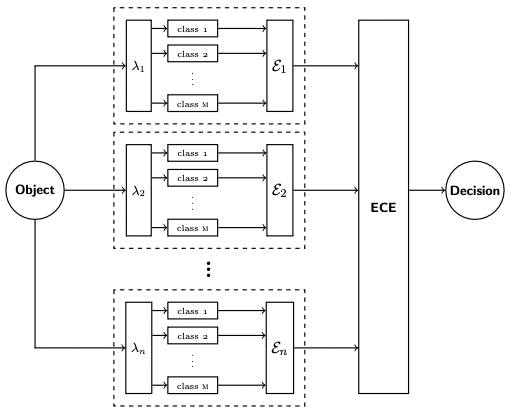
\includegraphics[width=\textwidth]{figures/ece}
	\caption{Schemat zespołu ekspozerów.}\label{fig:ece}
\end{figure}

% SKRÓĆ DWA AKAPITY PONIŻEJ I ZAPISZ TYLKO OGÓLNE WNIOSKI
Zaproponowana w pracy metoda została poddana ewaluacji z wykorzystaniem pakietu \emph{Weles}\sidenote{Weles -- Collection of various pattern recognition methods and experimental tools made by ML Group of Wrocław University of Science and Technology. --- \url{https://github.com/w4k2/weles}} opracowanego w ramach bieżących prac \emph{Zespołu Uczenia Maszynowego, Katedry Systemów i Sieci Komputerowych}. Jak można zauważyć dzięki przeprowadzonej analizie, \textsc{ece} często osiąga szczyt swojej efektywności przy relatywnie niskich wartościach hiperparametrów, jakkolwiek trudniejsze, wielowymiarowe i silnie niezbalansowane problemy przesuwają tę granicę wykazując, że wzrost próbkowania może mieć pozytywny wpływ na jakość klasyfikacji. W większości przypadków proponowane rozwiązanie osiąga rezultaty istotnie lepsze od pozostałych modeli bazowych, w żadnym przypadku nie okazując się najsłabszą metodą w stawce.

Algorytm \textsc{ece} wykorzystując informację o rozkładzie klas wykazuje przewagi typowe z klasyfikatorów bayesowskich, osiągając najlepsze rezultaty dla danych niezbalansowanych. Dodatkowo, dzięki strategii próbkowania podprzestrzennego pozostaje on w dużym stopniu odporny na zjawisko klątwy wielowymiarowości, ponieważ obiekty interpretowane są w nim jedynie w niskowymiarowych reprezentacjach. Łącząc te przewagi z regułą inferencyjną typową dla klasyfikatorów minimalnoodległościowych okazuje się on stabilnym rozwiązaniem dla trudnych przypadków danych jednocześnie niezbalansowanych i wielowymiarowych.  

\subsection*{II -- Algorytmy przetwarzania danych niezbalansowanych}

\marginnote{\scalebox{.6}{\large
	\def\imbcircle{(-210:2) circle (2.725cm)}
	\def\dscircle{(-330:2) circle (2.725cm)}
	\def\mdcircle{(-90:2) circle (2.725cm)}

	\begin{tikzpicture}
      	
      	\node[fill=black,rotate=0, text width=5.25cm, text height=2.9cm] at (90:-.5) {};
		\node[color=white,fill=black,rotate=0,rounded corners=.25cm, text width=5.25cm, align=center] at (90:1.25) {\bfseries \textsc{dane niezbalansowane}};
      	
      	\draw[fill=white] \mdcircle;
      	\draw[ultra thick] \mdcircle;
      	
      	\node at (-90:.5) {[C8]};    
      	\node at (-90:1.25) {[C6]};          	
      	    	   
      	\node at (-90:2) {\color{black!50}\emph{[C2]}};   
      	\node at (-90:2.75) {\color{black!50}\emph{[C3]}};   
      	\node at (-90:3.5) {\color{black!50}\emph{[C4]}};   
      	\node at (-90:4.25) {\color{black!50}\emph{[C9]}};
	\end{tikzpicture}}}

Drugim istotnym wątkiem moich prac realizowanych po uzyskaniu stopnia naukowego doktora jest przetwarzanie danych niezbalansowanych. Elementy tego rodzaju przetwarzania obecne są już w pracach przedstawionych we wcześniejszej sekcji, ale wyodrębniłem też w badaniach jednoznaczny wątek traktujący ten problem jako podstawowe zagadnienie analiz.

Po prawej stronie diagram zaznaczający opisywane w ramach wątku przetwarzania danych niezbalansowanych, wliczający prace opisane w~innych wątkach dominujących.
\vspace{1em}

{
\color{red}
\noindent\begin{tabular}{p{\textwidth}}
	\toprule &
\end{tabular}\vspace{-1em}
}
\noindent Przykładem takiego podejścia jest praca \citeC[-2.25em]{C6}, proponująca hybrydowe rozwiązanie łączące dywersyfikację podprzestrzenną z nadpróbkowywaniem syntetycznym. Strategia taka pozwala na budowę zespołu klasyfikatorów integrującego oversampling w procedurze konstrukcji systemu wieloklasyfikatorowego w miejsce stosowanego standardowo potoku rozłącznych akcji \emph{preprocessing $\rightarrow$ modelowanie}. W typowym podejściu do konstrukcji tego rodzaju systemów, faza preprocessingu nie jest specyficzna dla dywersyfikowanych modeli, a dokonuje się przed uróżnorodnieniem puli.

Konstrukcja dowolnego zespołu klasyfikatorów wiąże się z~dwiema podstawowymi trudnościami. Pierwszą jest zapewnienie różnorodnej puli klasyfikatorów pozwalającej na realizację niezależnych predykcji. Możemy osiągnąć to przez wykorzystywanie różnych modeli -- w~ramach dywersyfikacji heterogenicznej -- lub też przez modyfikację zestawu danych treningowych -- przy bardziej czytelnej w integracji dywersyfikacji homogenicznej. Proponowana metoda wykorzystuje to drugie podejście, w~którym każdy klasyfikator jest trenowany na losowej podprzestrzeni zbioru uczącego. Redukcja przestrzenności problemu, poza zapewnieniem różnorodności, stanowi również czynnik różnicujący efekt nadpróbkowywania. Standardowe metody syntetycznego oversamplingu, takie jak \textsc{smote}~\citeZ{Z25} czy \textsc{adasyn}, opierają się najczęściej na ocenie podobieństwa wzorców określanego przez metryki dystansowe, którego struktura zmienia się wraz z~każdą modyfikacją zbioru uczącego inną niż losowy obrót przestrzeni problemu~\citeZ{Z24}.

Drugą trudnością typową dla projektowania zespołu klasyfikatorów jest zapewnienie odpowiedniej reguły decyzyjnej, integrującej predykcje modeli dostępnych w puli. Najbardziej obiecującym rozwiązaniem w tym wypadku -- pozwalającym na przekroczenie ograniczenia abstrakcyjnej reguły decyzyjnej Wyroczni\footnote{Wyroczna -- w zakresie uczenia zespołowego -- stanowi abstrakcyjną regułę decyzyjną o nieuprawnionym dostępie do etykiet, podejmującą słuszną decyzję zawsze, kiedy skłania się ku niej co najmniej jeden z klasyfikatorów w puli.} stawianego regułom opartym na głosowaniu większościowym -- jest akumulacja wsparć klasyfikatorów bazowych. Należy jednak pamiętać, że wymaga ona wykorzystania wyłącznie klasyfikatorów udostępniających funkcję decyzyjną, klasyfikatorów problabilistycznych lub modeli o interpretacji probabilistycznej. Regułę taką można dodatkowo rozbudować przez wprowadzenie ważenia, które w rozważanym przypadku oparte było na wyznaczonej przez metrykę $F_1$ jakości osiąganej przez każdy z modeli wchodzących w skład puli.

Pełen schemat przetwarzania zaproponowanej metody przedstawiony został na Rysunku~\ref{fig:hais}. Zgodnie z przedstawioną procedurą, dostępny zbiór uczący dzielony jest na podzbiory jego atrybutów, a następnie obiekty klasy mniejszościowej każdej zredukowanej tak reprezentacji są syntetyzowane do poziomu zbalansowania przez algorytm \textsc{smote}, aby na każdej lokalnie zrównoważonej reprezentacji zbudować nowy model. Tak skonstruowana pula klasyfikatorów integrowana jest później przez akumulację wsparć ważoną przez wartość metryki $F_1$ osiągniętej na pełnym zbiorze uczącym.

\begin{figure}[h]
	\centering
	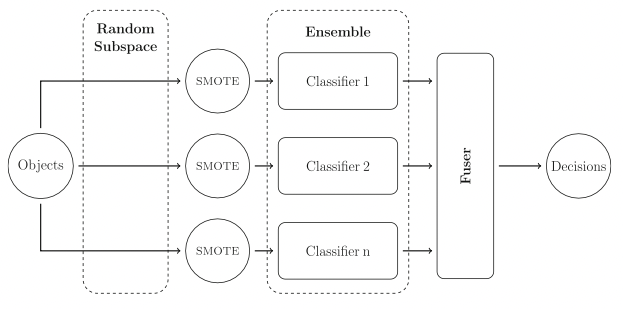
\includegraphics[width=\textwidth]{figures/hais}
	\caption{Schemat architektury zespołu klasyfikatorów zaproponowanego w pracy \emph{Combining Random Subspace Approach with \textsc{smote} Oversampling for Imbalanced Data Classification}.}\label{fig:hais}
\end{figure}

Zaproponowana metoda została poddana ewaluacji eksperymentalnej z wykorzystaniem 30 zbiorów danych o różnej, wysokiej skali niezbalansowania, dostępnych w repozytorium \textsc{keel}\sidenote[][]{Knowledge Extraction Evolutionary Learning -- dataset repository\\\noindent\url{https://sci2s.ugr.es/keel/datasets}}. W ramach ewaluacji przetestowano efektywność rozwiązania dla trzech klasyfikatorów o~interpretacji probabilistycznej: \emph{Gaussian Naive Bayes}, \emph{Logistic Regression} i~\emph{Support Vector Machine}. Analiza miała na celu porównanie ze sobą sześciu podejść:

\begin{itemize}
	\item uczenia na oryginalnym zbiorze,
	\item globalnego oversamplingu \textsc{smote},
	\item dywersyfikacji przez losowe podprzestrzenie,
	\item połączenia dywersyfikacji przez losowe podprzestrzenie z lokalnym oversamplingiem \textsc{smote},
	\item ważonego przez metrykę \emph{F1-score} zespołu o surowej dywersyfikacji przez losowe podprzestrzenie,
	\item ważonego przez metrykę \emph{F1-score} zespołu łączącego dywersyfikację przez losowe podprzestrzenie z lokalnym oversamplingiem \textsc{smote}.
\end{itemize}

Analiza uzyskanych wyników pozwala zaobserwować, że niezależnie od wykorzystanego klasyfikatora bazowego, użycie globalnego oversamplingu \textsc{smote} wpływa pozytywnie na jakość rozpoznawania, z reguły ulepszając model bazowy. 

Patrząc na drugi istotny czynnik przetwarzania, wykorzystanie jedynie dywersyfikacji przez losowe podprzestrzenie, przy warunkach wysokiego niezbalansowania, prowadzi do bardzo niskich rezultatów, pogarszających nawet jakość klasyfikatora bazowego. Wprowadzenie ważenia zespołu ulepsza taki model, prowadząc do rezultatów lepszych niż bazowy, ale nadal gorszych niż globalny \textsc{smote}.

Wykorzystanie obydwu tych strategii, w formie zespołu z lokalnym nadpróbkowywaniem, prowadzi do rezultatów odrobinę lepszych niż globalny \textsc{smote}, co może sugerować, że pozytywny wpływ obu tych czynników jest niezależny od siebie i potencjalnie może okazać się komplementarny. Potwierdzają to rezultaty osiągane przez pełną propozycję rozwiązania, ważony zespół łączący dywersyfikację przez losowe podprzestrzenie z lokalnym oversamplingiem, którego jakość jest jednoznacznie najlepsza w puli analizowanych przykładów.

Praca uprawdopodabnia stwierdzenie, że wspólne wykorzystanie metod balansowania i dywersyfikacji, przy kontroli wpływu każdej podprzestrzeni na finalną predykcję przez ważenie zgodne z efektywnością w problemie niezbalansowanym, może prowadzić do zbliżenia się do optymalnego rozmieszczenia obiektów uczących w przestrzeni problemu i tym samym prowadzić do budowy modeli o wysokiej zdolności dyskryminacyjnej.\vspace{1em}

\newpage
{
\color{red}
\noindent\begin{tabular}{p{\textwidth}}
	\toprule &
\end{tabular}\vspace{-1em}
}
\noindent Wykorzystanie metod resamplingu w konstrukcji systemów rozpoznawania dla danych niezbalansowanych nierozerwalnie niesie ze sobą ryzyko utraty informacji o potencjalnie istotnych obiektach klasy większościowej. Możliwa jest jednak mitygacja tego problemu, przez odpowiednie wykorzystanie podejścia zespołowego, które pozwoli na pełne wykorzystanie dostępnych danych bez konieczności syntetyzacji nowych wzorców lub redukcji obiektów istniejących. Propozycję algorytmu tego rodzaju przedstawiłem w pracy \citeC[-12em]{C8}.

Metoda ta dedykowana jest jedynie problemom binarnym o wysokim stopniu niezbalansowania, gdzie \emph{imbalanced ratio} (\textsc{ir}) wynosi 1:9 i~więcej. Złożone metody resamplingu, takie jak \textsc{smote} czy \textsc{adasyn}, pomimo wysokiej efektywności w~wielu niezbalansowanych problemach rozpoznawania, nie odnajdują swojego zastosowania w~scenariuszach skrajnych, gdzie klasa mniejszościowa reprezentowana jest jedynie przez kilka przykładów pośród których nie jest możliwa analiza sąsiedztwa pozwalająca na syntetyzację nowego obiektu. Teoretycznie możliwe jest w~takiej sytuacji zastosowanie undersamplingu, ale jak pokazują badania, rozwiązania takie w sytuacjach silnego niezbalansowania nie pozwalają na uzyskanie stabilnego systemu rozpoznawania.

Popularnym rozwiązaniem w takiej sytuacji jest wykorzystanie standardowych zespołów opartych na \emph{Baggingu} lub \emph{Boostingu} -- opartych na losowym próbkowaniu ze zwracaniem, które pozwalają na rozbicie dużego problemu w~serię mniejszych. W~pracy proponuję prostą obliczeniowo metodę, która również dokonuje rozbicia problemu rozpoznawania, zapewniając jednak obecność wszystkich obiektów dostępnych w~zbiorze uczącym, eliminując również ryzyko nakładania się klas.

Model \emph{Undersampled Majority Class Ensemble} (\textsc{umce}) buduje się zgodnie z następującymi krokami:

\begin{fullwidth}\vspace{2em}
\hspace{1em}\begin{minipage}{30em}
\begin{itemize}
	\item[1.] Podziel $\mathcal{DS}$ na zbiór mniejszościowy $MinC$ i większościowy $MajC$.
	\item[2.] Wyznacz współczynnik niezbalansowania $IR$ jako proporcję liczności zbiorów $MinC$ i $MajC$.
	\item[3.] Wyznacz współczynnik $k$ jako najbliższe całkowite zaokrąglenie $IR$.
	\item[4.] Zrealizuj k-foldowy podział zbioru $MajC$, aby wytworzyć zbiór podzbiorów $MajC_1, MajC_2, \ldots, MajC_k$.
	\item[5.] Dla każdego $i$ w zakresie do $k$:
	\begin{itemize}
		\item[6.] Złącz zbiory $MajC_i$ i $MinC$ w zbalansowany zbiór $\mathcal{TS}_i$.
		\item[7.] Zbuduj model $\Psi_i$ na podstawie przykładów $\mathcal{TS}_i$ i dodaj go do zespołu.
	\end{itemize} 
\end{itemize}
\end{minipage}\vspace{2em}
\end{fullwidth}

Opcjonalnym elementem przetwarzania jest uzupełnienie puli modeli o dodatkowy klasyfikator zbudowany z wykorzystaniem typowego zastosowania algorytmu \textsc{smote}. Został on włączony do metody aby umożliwić weryfikację różnic w zyskach z obu strategii, podobnie jak miało to miejsce w poprzednio opisanej pracy.

Klasycznie już, istotnym elementem metody zespołowej jest również reguła integracji. W wypadku algorytmu \textsc{umce} zdecydowałem się odejść od prostych paradygmatów fuzji wsparć, rozwijając strategię podstawową (\textsc{reg}) i ważoną proporcjonalnie do jakości (\textsc{wei}) o trzy dodatkowe propozycje:

\begin{itemize}
	\item[\bfseries\textsc{nor}] \textbf{Normalizowana przedziałowo akumulacja ważona} -- pozwalająca na istotne wzmocnienie najlepszego klasyfikatora w puli i całkowitą redukcję wpływu klasyfikatora najsłabszego.
	\item[\bfseries\textsc{con}] \textbf{Dynamiczna akumulacja wsparć}. Aby zapewnić lepsze wykorzystanie klasyfikatorów o większej "pewności" decyzji względem danego obiektu, decyzja dla każdego wzorca ważona jest przez bezwzględną różnicę pomiędzy wsparciami, która na potrzeby badań została nazwana \emph{kontrastem}. Ilustracją tego podejścia jest Rysunek~\ref{fig:contrast}, na osiach X prezentujący próbki, a na osiach Y -- klasyfikatory dostępne w puli. Białe punkty pokazują kontrast 1, a więc decyzję pewną, podczas gdy czarne powiązane są z kontrastem 0, a więc absolutnym brakiem pewności, czyli wzorcem leżącym bezpośrednio na granicy decyzyjnej.
	\item[\bfseries\textsc{nci}] \textbf{Akumulacja wsparć ważona przez iloczyn \textsc{nor} i \textsc{con}}.
\end{itemize}

\begin{figure}[!htb]
	\vspace{-1em}\centering
	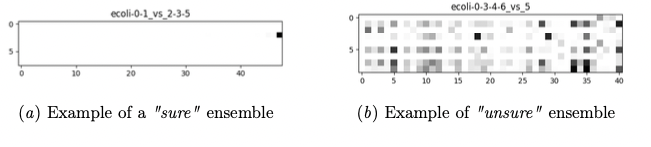
\includegraphics[width=\textwidth]{figures/contrast}
	\caption{Ilustracja rozkładu \emph{kontrastu} w zespołach klasyfikatorów zbudowanych na dwóch zbiorach danych.}\label{fig:contrast}
	\vspace{-2em}
\end{figure} 

Należy pamiętać, że zaproponowana metoda budowy zespołu uzależnia jego wielkość od poziomu niezbalansowania, co dla danych bardzo silnie niezbalansowanych (przykładowo o IR 1:100) prowadzić będzie do konstrukcji bardzo dużego modelu hybrydowego. W związku z tym, zaproponowana została również metoda przycinania zespołu klasyfikatorów.

Typowe metody przycinania zespołów działają w trybie statycznym, analizując jakość modeli członkowskich i wycinając pulę klasyfikatorów o najniższym potencjale dyskryminacyjnym. W pracy zaproponowałem jednak metodę przycinania dynamicznego, dostosowującego skład zespołu do zbioru testowego. Zespół, otrzymując na wejściu zbiór testowy, generuje wektory wsparć ($s_i$) dla każdego klasyfikowanego obiektu, co pozwala zinterpretować wsparcia dla danej klasy z danego klasyfikatora jako zmienne losowe możliwe do analizy wzajemnej zależności statystycznej. W propozycji, wykorzystując test rankingowy, dokonuję klasteryzacji puli $k$ modeli do $n$ grup ($n \leq k$) celem uśrednienia wsparć i wag w obrębie każdej grupy przed końcową integracją. 

Pełen schemat organizacji metody \textsc{umce} z rozbiciem na blok indukcyjny i predykcyjny przedstawiony został na Rysunku~\ref{fig:umce}.

\begin{figure}[!htb]
	\centering
	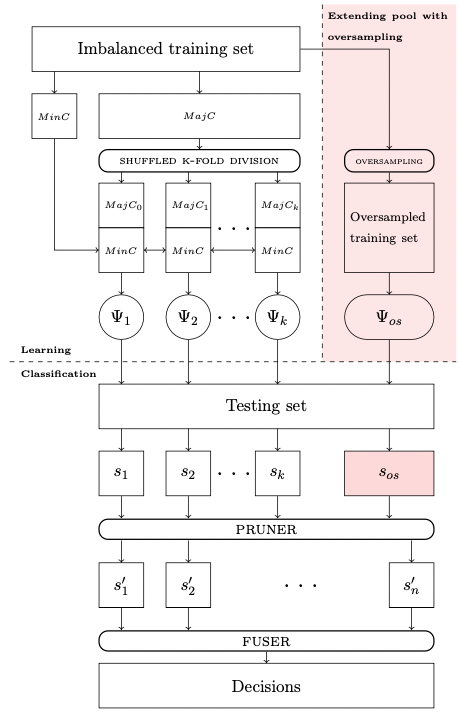
\includegraphics[width=.9\textwidth]{figures/umce}
	\vspace{-1em}
	\caption{Schemat organizacji metody \emph{Undersampled Majority Class Ensemble}.}\label{fig:umce}
\end{figure}

Ewaluacja eksperymentalna metody \textsc{umce} została zrealizowana na 40 binarnych problemach klasyfikacji o \textsc{ir} większym niż 1:9. Aby umożliwić właściwe porównanie z metodami referencyjnymi zastosowano klasyczną, pięciofoldową walidację krzyżową, a w ocenie jakości modeli zastosowana została metryka zbalansowanej dokładności.

Metoda bazowa osiągnęła przewagę nad konkurencją jedynie w~trzech przypadkach, podczas gdy standardowe metody over- i~undersamplingu okazały się najlepsze w~nie więcej niż dwóch przypadkach, niezależnie od zastosowanego klasyfikatora bazowego. Jednak, zarówno rozszerzenie puli klasyfikatorów \textsc{umce} o~model wykorzystujący \textsc{smote}, jak i~zaproponowana metoda pruningu oraz mieszana metoda ważenia \textsc{nci} prowadzą do jednoznacznie najlepszych rezultatów w~porównaniu. Należy podkreślić skuteczność metody \textsc{umce} tym bardziej, że nawet najprostsza forma jej architektury, pozbawiona przycinania i~ważenia zespołu, osiąga wyniki istotnie lepsze niż metody \emph{state-of-the-art} dziedziny.

\subsection*{III -- Algorytmy przetwarzania strumieni danych}

\marginnote{\scalebox{.6}{\large
	\def\imbcircle{(-210:2) circle (2.725cm)}
	\def\dscircle{(-330:2) circle (2.725cm)}
	\def\mdcircle{(-90:2) circle (2.725cm)}

	\begin{tikzpicture}
      	
      	\node[fill=black,rotate=0, text width=5.25cm, text height=2.9cm] at (90:-.5) {};
		\node[color=white,fill=black,rotate=0,rounded corners=.25cm, text width=5.25cm, align=center] at (90:1.25) {\bfseries \textsc{strumienie danych}};
      	
      	\draw[fill=white] \mdcircle;
      	\draw[ultra thick] \mdcircle;
      	
      	% 10 9 11 
      	% MD
      	\node at (-90:0) {[C7]};
      	\node at (-90:.75) {[C4]};    
      	\node at (-90:1.5) {[C3]};    
      	\node at (-90:2.25) {[C5]};    
      	\node at (-90:3) {[C2]};    
      	\node at (-90:3.75) {[C1]};
	\end{tikzpicture}}}

Po prawej stronie diagram zaznaczający opisywane w ramach wątku przetwarzania strumieni danych, wliczający prace opisane w innych wątkach dominujących.

Istnieje wyraźne podobieństwo pomiędzy wsadowym podejściem do predykcji, wykorzystywanym w procedurze przycinania algorytmu \textsc{umce}, a typowymi strategiami przetwarzania strumieni danych, które swoją ewaluację opierają na protokole \emph{Test-Then-Train}. Środowisko tego rodzaju pozwala nie tylko na wnioskowanie względem pojedynczego predykowanego obiektu, ale też udostępnia kontekst, w którym obiekt ten pojawia się w toku przetwarzania. Rozwiązania takie stanowią trzeci, kluczowy wątek prac realizowanych przeze mnie w ramach omawianego cyklu publikacji podejmującego tematykę klasyfikacji danych trudnych.\vspace{1em}

{
\color{red}
\noindent\begin{tabular}{p{\textwidth}}
	\toprule &
\end{tabular}\vspace{-1em}
}
\noindent Pierwszą omawianą pracą z tej kategorii jest artykuł~\citeC[-2.25em]{C7}. Podejmuje on tematykę wykorzystania efektu \emph{catastrophic forgetting} -- typowego dla sieci neuronowych -- w adaptacyjnej klasyfikacji strumieni danych podatnych na zjawisko dryfu koncepcji przy redukcji zaangażowania ekspertów w uzyskiwaniu oznaczenia danych. 

Strategie uczenia się przy ograniczonej etykietyzacji dla problemów stacjonarnych, często opierają się na klasteryzacji dostępnych obiektów pozwalającej na transdukcyjną identyfikację prototypów, które po oznaczeniu przez eksperta stanowią później przypadki reprezentatywne dla wydzielonych podzbiorów zbioru uczącego. W wypadku uczenia inkrementalnego i strumieniowego częściej jednak wykorzystywany jest paradygmat uczenia aktywnego, w którym pewna wiedza -- zakumulowana już przez przyrostowy model -- może być wykorzystywana do identyfikacji tzw. przypadków trudnych w obrębie nowego, nieoznaczonego jeszcze wsadu.

Podstawowym zagadnieniem poruszanym w pracy jest istotna redukcja kosztów konstrukcji systemu rozpoznawania w środowisku strumieniowym przy jednoczesnym zachowaniu efektywności, którą uzyskałby przy pełnym dostępie do etykiet. W wielu zadaniach praktycznych niemożliwe jest pozyskanie odpowiedniego zbioru etykiet w racjonalnym czasie, a jednocześnie niemal zawsze wymaga ona wykorzystania czynnika ludzkiego, który jest zarówno kosztowny, jak i omylny -- szczególnie jeżeli dotyczy oznaczania danych masowych i napływających z~wysoką częstotliwością. Sprawia to, że projektowanie metod klasyfikacji, które zdolne są do budowy rzetelnych systemów rozpoznawania przy jedynie częściowej etykietyzacji jest jednocześnie dużym wyzwaniem, jak i~nadal bardzo pożądanym celem badań. W~ramach pracy proponowany jest hybrydowy model uczenia aktywnego, łączący podejścia typowe dla uczenia online wraz ze strategiami okna przesuwnego.

Przyjmujemy, że jeżeli decyzja dla zadanego obiektu wynika z wysokiej wartości wsparcia, leży on daleko od granicy decyzyjnej, a więc wykorzystanie go w budowie modelu nie będzie mieć istotnego wpływu na zmianę estymowanego prawdopodobieństwa \emph{a posteriori}. W wypadku modeli interpretowanych probabilistycznie wysoka wartość funkcji wsparcia oznacza też niewielkie prawdopodobieństwo błędu klasyfikacji. Stąd znacznie bardziej~"\emph{interesujące}"~dla procedury modelowania są przypadki trudne, o niepewnej decyzji -- rozumianej jako niewielka różnica pomiędzy wsparciami dla kategorii konkurujących między sobą o decyzję eksperta. 

Aby sformalizować to założenie, zaproponowana została funkcja $RSFD$ (\emph{Relative Support Function Difference}), mierząca średnią różnicę pomiędzy największym prawdopodobieństwem i każdym z pozostałych elementów wektora wsparć dla zadanej obserwacji $x$

\begin{equation}
	RSFD(x) = \frac{\sum_{i=1}^{M}[ \max_{k\in\mathcal{M}}(F_k(x)) - F_i(x)]}{M-1},
\end{equation}

\noindent gdzie $Fi(x)$ to wartość wsparcia klasyfikatora $i$ dla obiektu $x$. 

Graficzna interpretacja funkcji $RSFD$ dla przypadku dwu- i trzyklasowego zaprezentowana jest również na Rysunku~\ref{fig:neuro1}. Barwy na ilustracji prezentują wsparcia dla klas, a spadek wartości w podglądzie monochromatycznym -- trudność przypadków objętych obszarem.

\begin{figure}[!htb]
	\centering
	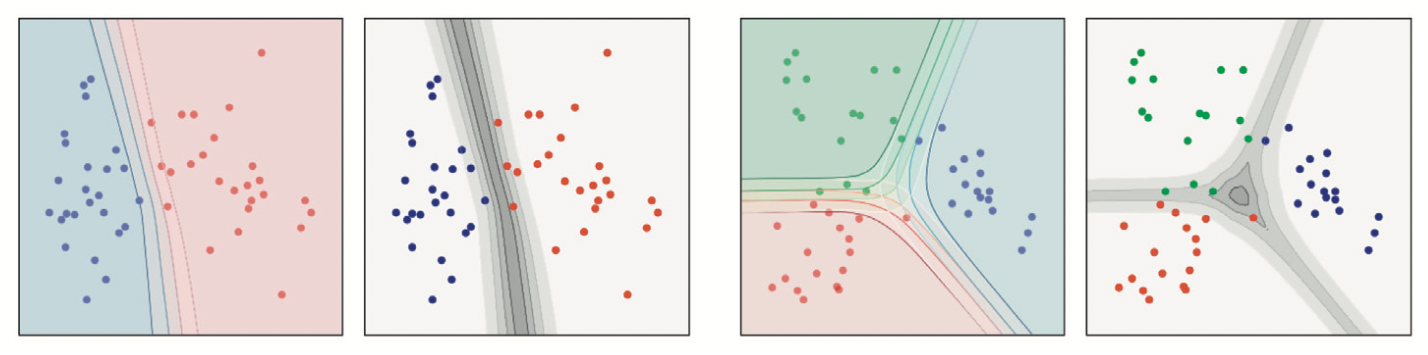
\includegraphics[width=\textwidth]{figures/neuro1}
	\caption{Przykład rozkładu wsparć i wartości funkcji RSFD dla dwuwymiarowych zbiorów o dwóch i trzech klasach problemu.}\label{fig:neuro1}
\end{figure}

Klasycznie, podejście takie wykorzystywane jest w~\emph{klasyfikacji z~opcją odrzucenia} (ang. \emph{classification with reject option}\citeZ{Z26}), gdzie decyzje podejmowane są jedynie dla przypadków względem których klasyfikator jest w stanie podjąć dostatecznie pewną decyzję. W proponowanym przetwarzaniu zasada ta jest jednak odwracana i~fakt \emph{odrzucenia} danego obiektu jest powiązany z~identyfikacją go jako obserwacji interesującej i~skierowaniem do oznaczenia przez eksperta. Celem umożliwienia kontroli tego procesu wprowadzone zostały dwa hiperparametry metody:

\begin{itemize}
	\item \emph{próg} -- wprowadzający wartość graniczną średniej różnicy wsparć, poniżej której obiekt uznawany jest za interesujący,
	\item \emph{budżet} -- określający jaki największy odsetek wsadu uczącego może zostać skierowany do etykietyzacji.
\end{itemize}

Całość zrealizowanej ewaluacji eksperymentalnej, jak w większości wchodzących w skład cyklu prac podejmujących przetwarzanie strumieniowe, wykonana została w oparciu o model \emph{Multilayer Perceptron}. Efekty przeprowadzonej analizy pozwoliły na uprawdopodobnienie hipotezy o możliwości znaczącej redukcji kosztu etykietyzacji przy jednoczesnym zachowaniu zdolności dyskryminacyjnej modeli strumieniowych. Wstępne badania wykazały, że proste podejście budżetowe, pomijające całkowicie aspekt aktywnego doboru wzorców do etykietyzacji, liniowo degraduje krzywą uczącą, istotnie wydłużając czas konwergencji modelu. Wykorzystanie tej samej, lub nawet niższej liczby wzorców, dobranych jednak zgodnie z sugestiami dotychczasowego modelu, niweluje ten efekt, często pozwalając nawet na eliminację zapotrzebowania na eksperta w stabilnej fazie koncepcji. 

Co szczególnie interesujące i~możliwe do zaobserwowania w~eksperymentach rozszerzonych, osiągany efekt w~niektórych przypadkach pozwala nie tylko na zachowanie zdolności dyskryminacyjnych modelu o pełnej etykietyzacji, ale też wykazuje zdolność do eliminacji obiektów o~negatywnym wpływie na model i~prowadzi do osiągnięcia wcześniejszej zbieżności sieci neuronowej. Pokazuje to, że dziedzina przetwarzania strumieni danych nadal jest obszarem o~dużym potencjale rozwijania badań, w~szczególności tych dotyczących budowy modeli neuronowych w~środowiskach o~zmiennych koncepcjach.

Najpowszechniej podejmowanym w literaturze obszarem badań z~zakresu strumieni danych jest analiza zdolności systemów uczących się do adaptacji do zmian w~prawdopodobieństwie a posteriori problemu, a~więc do dryfu koncepcji. Interesującym badawczo obszarem jest jednak również punkt styku pomiędzy tą tematyką, a~problemem niezbalansowania danych, zdefiniowanym jako jeden z~trzech głównych obszarów tematycznych prezentowanego cyklu.\vspace{1em}

{
\color{red}
\noindent\begin{tabular}{p{\textwidth}}
	\toprule &
\end{tabular}\vspace{-1em}
}
\noindent Analizując to zagadnienie, w artykule~\citeC[-2.25em]{C4} wykazałem, że możliwe jest uwzględnienie estymowanego prawdopodobieństwa a priori strumienia danych o stałym stopniu niezbalansowania w istotnym statystycznie polepszeniu mocy generalizacyjnej modeli rozpoznawania. Podstawą analizy była weryfikacja potencjału przetwarzania końcowego (\emph{postprocessingu}) w ulepszaniu modelu klasyfikacji strumieni niezbalansowanych statycznie bez ingerowania w procedurę budowy modelu.

W ramach pracy zaproponowana została metoda \emph{Prior Imbalance Compensation} (\textsc{pic}), generująca stosunkowo minimalny narzut obliczeniowy i zaprojektowana dla strumieni, w których nowe instancje pojawiają się z wysoką częstotliwością i w dużych ilościach lub dla przypadków o bardzo dużej skali niezbalansowania (w której odsetek klasy mniejszościowej stanowi mniej niż 5\% ogółu dostępnych danych). Tak silne zaburzenie proporcji pomiędzy klasami, jak wskazane zostało już w opisie metody \textsc{umce}, uniemożliwia syntetyzację wzorców metodą \textsc{smote}, a~więc wymaga alternatywnych strategii przetwarzania.

Algorytm \textsc{pic}, na podstawie dotychczas etykietowanych przypadków, przy najbardziej typowym dla literatury założeniu o stabilności niezbalansowania, z rosnącą precyzją estymuje prawdopodobieństwa \emph{a priori} przetwarzanego problemu. Estymacja ta nie jest wykorzystywana przy budowie modelu, która odbywa się w klasyczny sposób, ale stanowi podstawę dla korekty uwzględnianej przy predykcji wsadowej. Jest ona możliwa do realizacji dla dowolnego modelu o interpretacji probabilistycznej lub o ciągłych funkcjach decyzyjnych, a więc przetestowana została w oparciu o klasyfikatory \emph{Naive Bayes}, \emph{k-Nearest Neighbors}, \emph{Random Trees} oraz \emph{Support Vector Machine}.

Zrealizowana ewaluacja eksperymentalna oceniała efektywność klasyfikacji strumieni niezbalansowanych (przetestowano problemy od zbalansowanych do niezbalansowanych w skali 1:20) zgodnie ze wskazaniami metryk zbalansowanej dokładności i \emph{F1-score}. Kompensacja aprioryczna \textsc{pic} pozwoliła na uzyskanie istotnego statystycznie polepszenia zbalansowanej dokładności klasyfikacji z niewielkim spadkiem metryki \emph{F1-score} w każdym z testowanych scenariuszy. Szczególnie wyraźne jest to dla modeli opartych o \emph{Support Vector Machine}.

%\begin{table}[!htb]
%	\centering
%	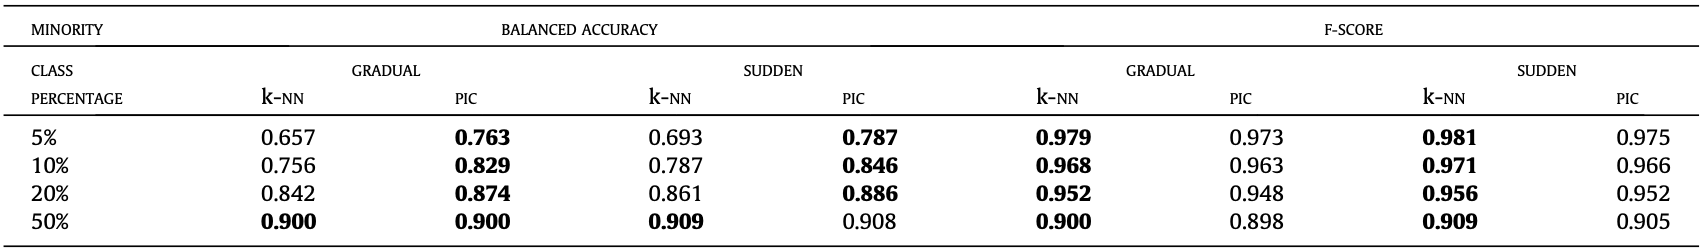
\includegraphics[width=\textwidth]{figures/pic}
%	\caption{Zbalansowana dokładność i miara F-score dla strumieni niezbalansowanych o rosnącym współczynniki niezbalansowania.}\label{tab:pic}
%\end{table}

Korekta aprioryczna ma też pewien wpływ na klasyfikację strumieni zbalansowanych, ale stanowi ona wtedy tylko niewielkie zaburzenie w~jakości. Wraz ze zwiększaniem się skali niezbalansowania, przy zachowaniu tych samych analizowanych koncepcji, widać wyraźną degenerację modeli bazowych w~domyślnej interpretacji predykcji przy jednoczesnym zachowaniu wysokiej sprawności przy zastosowaniu \textsc{pic}. Należy zaznaczyć, że w~obu przypadkach wykorzystywany jest dokładnie ten sam model, poddany jednak zmienionej interpretacji funkcji decyzyjnej.

Zbliżone obserwacje zostały dokonane zarówno na dryfach gradualnych, jak i~nagłych. Algorytm \textsc{pic} jest zdolny do ulepszenia jakości rozpoznawania dla każdego z~rozważanych modeli klasyfikacji, ale największą odporność na niezbalansowania uzyskują dzięki niemu \emph{Support Vector Machine}.\vspace{1em}

{
\color{red}
\noindent\begin{tabular}{p{\textwidth}}
	\toprule &
\end{tabular}\vspace{-1em}
}
\noindent Rozszerzone badania nad potencjałem metody \textsc{pic} pozwoliły na wstępną identyfikację nowego obszaru badawczego w zakresie przetwarzania niezbalansowanych strumieni danych, które pogłębiłem w dwóch kolejnych publikacjach prezentowanych w ramach konferencji \emph{IEEE World Congress on Computational Intelligence 2021'}~\citeC[-8em]{C3} i \emph{2022'}~\citeM[.5em]{Kom22}, z których pierwsza -- z racji na istotne rozwinięcie tej koncepcji -- włączona została do opisywanego cyklu.

W pracy rozwijana jest analiza dotycząca przetwarzania niezbalansowanych strumieni danych z uwzględnieniem potencjalnej dynamiki tych zmian. Wraz ze współautorami proponujemy tam taksonomię zjawisk niezbalansowania strumieni danych, wydzielającą następujące kategorie:

\begin{itemize}
	\item[\textsc{bs}] \textbf{Strumienie zbalansowane (\emph{balanced streams})}, gdzie globalne prawdopodobieństwo \emph{a priori} i każde z prawdopodobieństw lokalnych jest proporcjonalne i wzajemnie zależne.
	\item[\textsc{sis}] \textbf{Strumienie niezbalansowane statyczne (\emph{statically imbalanced streams})}, gdzie globalne prawdopodobieństwo \emph{a priori} i prawdopodobieństwa dla każdego kolejnego okna sąsiadujących obiektów jest nieproporcjonalne, ale wzajemnie zależne.
	\item[\textsc{dis}] \textbf{Strumienie niezbalansowane dynamicznie (\emph{dynamically imbalanced streams})}, wśród których można wydzielić dwie kategorie:
	\begin{itemize}
		\item[\textsc{cdis}] \textbf{Strumienie niezbalansowane dynamicznie w sposób ciągły (\emph{continous dynamically imbalanced streams})}, gdzie globalne prawdopodobieństwo \emph{a priori} może różnić się od prawdopodobieństwa dla każdego kolejnego okna sąsiadujących obiektów, które nie są wzajemnie zależne, ale zmieniają się w sposób ciągły, umożliwiając obserwację trendów zmian.
		\item[\textsc{ddis}] \textbf{Strumienie niezbalansowane dynamicznie w sposób dyskretny (\emph{discrete dynamically imbalanced streams})}, gdzie globalne prawdopodobieństwo \emph{a priori} może różnić się od prawdopodobieństwa dla każdego kolejnego okna sąsiadujących obiektów, które nie są wzajemnie zależne i zmieniają się dyskretnie, uniemożliwiając obserwację trendów zmian. 
	\end{itemize}
\end{itemize}

Przykładowe przebiegi prawdopodobieństwa wystąpienia klasy mniejszościowej dla przyjętej taksonomii zaprezentowane są na Rysunku~\ref{fig:stream-taxonomy}. Jak można zauważyć, klasyczny przypadek strumienia niezbalansowanego, typowy dla literatury (\textsc{sis}) charakteryzuje się stabilną proporcją o niewielkiej wariancji na całym przebiegu przetwarzania. Strumień niezbalansowany dynamicznie w sposób dyskretny (\textsc{ddis}) również wykazuje pewną wartość oczekiwaną niezbalansowania, ale wariancja estymacji prawdopodobieństwa jest już w nim na tyle duża, że może mieć istotny wpływ na jakość modelu. Strumień niezbalansowany dynamicznie w sposób ciągły (\textsc{cdis}) wykazuje charakter pośredni pomiędzy \textsc{sis} i \textsc{ddis}, cechując się niską lokalną wariancją, przy wysokiej wariancji globalnej.

\begin{figure}[!htb]
	\centering
	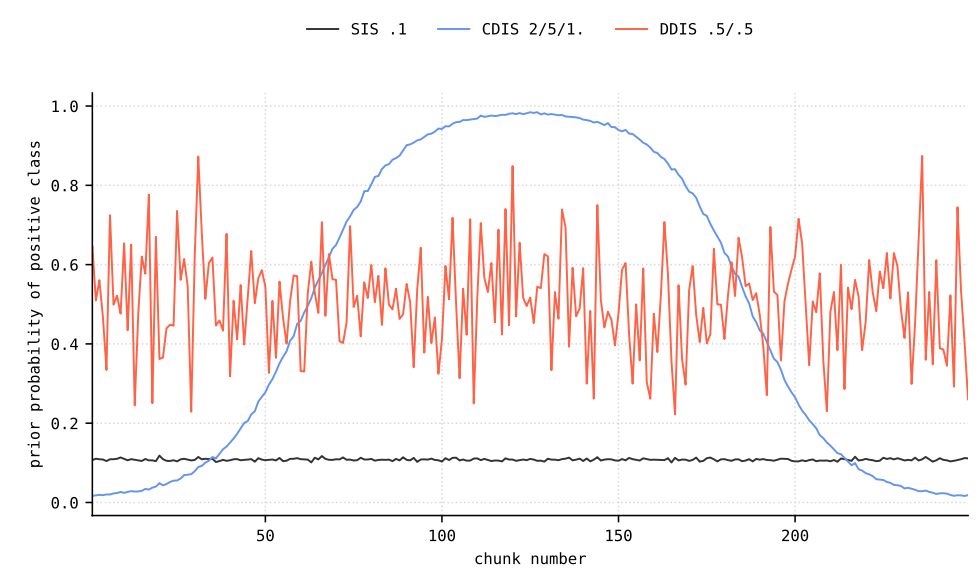
\includegraphics[width=\textwidth, clip=true]{figures/stream-taxonomy}
	\caption{Prawdopodobieństwo \emph{a priori} klasy pozytywnej dla kolejnych wsadów strumieni z każdej rozważanej kategorii strumieni niezbalansowanych.}\label{fig:stream-taxonomy}
\end{figure}

Opisywana praca -- poza taksonomią problemów -- proponuje również pulę rozwiązań standardowych oraz metodę nienadzorowanej estymacji prawdopodobieństwa \emph{a priori} zdolną do efektywnego rozpoznawania~w -- szczególnie trudnych -- strumieniach o niezbalansowaniu dyskretnie-dynamicznym (\textsc{ddis}). Algorytm \emph{Dynamic Statistical Concept Analysis} (\textsc{dsca}) wprowadza reprezentację koncepcji, jako zbioru jej standardowych miar statystycznych możliwych do wyznaczenia bez nadzoru etykiet, wraz z prostym zespołem regresorów sieci neuronowych. Modele regresji -- budowane dla każdej klasy problemu -- przy każdym kroku optymalizacji otrzymują tę samą reprezentację wsadu, jako zmienną objaśnianą przyjmując liczbę obiektów\sidenote[][-11em]{Wykorzystanie zespołu regresorów przyjmujących jako zmienną objaśnianą liczbę obiektów i integrującego końcową odpowiedź systemu przez proporcję -- w toku badań -- okazało się znacznie bardziej obiecującą strategią niż wyuczanie skali niezbalansowania. Podejście takie daje zarówno lepsze rezultaty, jak i umożliwia zastosowanie metody w~klasyfikacji wieloklasowej.} przypisanej im klasy. Zespół taki integrowany jest do wektora prawdopodobieństwa \emph{a priori} przez komplementarne skalowanie predykcji, pozwalając na późniejsze uwzględnienie w korekcie apriorycznej \textsc{pic}.

Dodatkowym elementem metody \textsc{dsca} jest dynamiczna kalibracja liczby epok uczenia, dostosowująca się do aktualnego poziomu błędu predykcji. W początkowej fazie przetwarzania wykonywanych jest więcej kroków optymalizacji -- celem szybkiego zyskania zbieżności modelu -- a z czasem wartość ta redukuje się do pojedynczych, korygujących aktualizacji (Rysunek~\ref{fig:dsca1}).

\begin{figure}[!h]
	\centering
	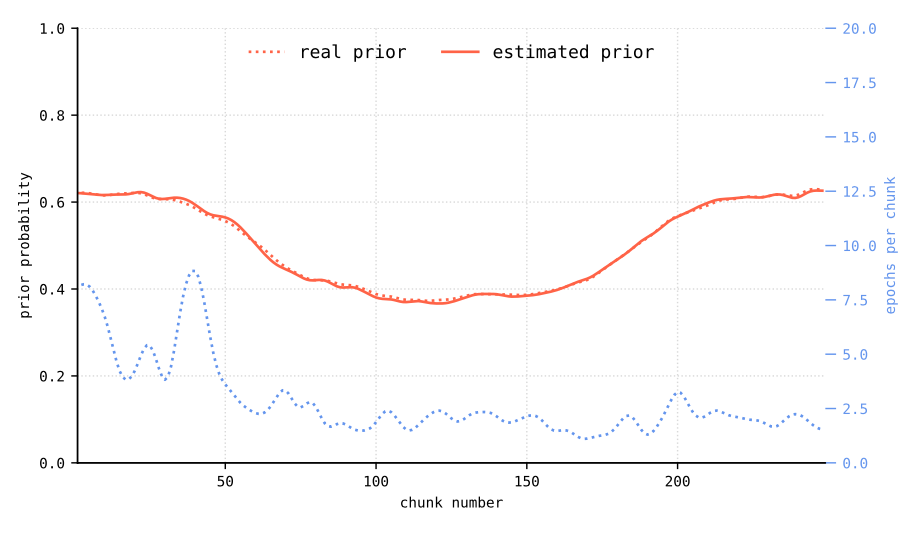
\includegraphics[width=\textwidth, clip=true]{figures/dsca1}
	\caption{Estymowane i rzeczywiste prawdopodobieństwo \emph{a priori} modelu DSCA zestawione z liczbą epok uczących regresory na wsad przetwarzania.}\label{fig:dsca1}
\end{figure}

Ewaluacja eksperymentalna metody przeprowadzona została z wykorzystaniem autorskiego generatora strumieni danych o dynamicznym niezbalansowaniu, który został zintegrowany z pakietem \emph{stream-learn}. W ramach testowanej hipotezy, badania weryfikowały możliwość zbudowania takiego modelu predykcji prawdopodobieństwa \emph{a priori}, który zdolny będzie do przewidywania w strumieniach niezbalansowanych dynamicznie w sposób dyskretny, w których standardowe podejścia będą wysoce niewydolne. Rezultaty pozwalają zaobserwować, że o ile w~wypadku strumieni niezbalansowanych statycznie nie występują istotne różnice w osiąganych rezultatach, to w niemal każdym ze scenariuszy dynamicznie-ciągłego niezbalansowania, metoda \textsc{dsca} okazuje się istotnie najlepszą w stosunku do wybranych metod referencyjnych. 

Szczególnie interesujący jest jednak przypadek wszystkich scenariuszy \textsc{ddis}, w których każda z metod referencyjnych wykazuje bardzo duży błąd -- proporcjonalny do wariancji w niezbalansowaniu. Algorytm \textsc{dsca} w takich przypadkach cechuje się bardzo wysoką efektywnością, podobną do osiąganej na pozostałych scenariuszach, okazując się jedyną dostępną obecnie w literaturze metodą odporną na niefunkcyjne zmiany w stopniu niezbalansowania.

Dalsze prace z zakresu predykcji prawdopodobieństwa \emph{a priori}, wykorzystujące zaproponowany model \textsc{dsca}, pozwoliły na uogólnienie obserwacji poczynionych wstępnie dla algorytmu \textsc{pic}, względem ogólnego modelu \emph{Multilayer Perceptron} w inkrementalnym przetwarzaniu danych.\vspace{1em}
\newpage

{
\color{red}
\noindent\begin{tabular}{p{\textwidth}}
	\toprule &
\end{tabular}\vspace{-1em}
}
\noindent Badania z zakresu przetwarzania strumieni danych często odnajdują również swoje zastosowania praktyczne. Przykładem takiego zastosowania zajmuje się praca~\citeC[-5em]{C5}, która stanowi pierwszą podjętą w literaturze przedmiotu analizę wykorzystania metod strumieniowych w zagadnieniu detekcji źródeł dezinformacji, a precyzyjnie, wykrywania treści wpisujących się w zjawisko fake news. 

Środowisko naukowe nie przyjęło jeszcze jednoznacznej i powszechnej definicji zjawiska \emph{fake news}~\citeM{Cho21}. W związku z tym, w badaniach podejmujących ten temat opieram się na określeniu go jako: \emph{treści niezgodnej z konsensusem przyjętym w określonej grupie społecznej, mającej za zadanie zmienić ten konsensus w sposób działający na niekorzyść tej grupy}.

Opisywana praca dokonuje przeglądu standardowych modeli rozpoznawania dla środowisk strumieniowych (\emph{Hoeffding Trees}, \emph{Multilayer Perceptron}, \emph{Naive Bayes}), w kontekście przetwarzania z wykorzystaniem trzech standardowych strategii budowy modeli. Analizowana jest w niej jakość (\emph{a}) modeli pojedynczych, (\emph{b}) klasycznych zespołów zbudowanych zgodnie z procedurą \textsc{sea}\sidenote[][-4em]{\emph{Streaming Ensemble Algorithm} --- podstawowy, prosty model zespołu klasyfikatorów o ustalonym limicie puli i jakościowym kryterium jej przycinania.} oraz (\emph{c}) modelu \emph{Online Bagging}, dobierającego wagi dla wzorców na podstawie rozkładu Poissona.

Ewaluacja eksperymentalna podjęta została w oparciu o zbalansowany zbiór danych \emph{Getting Real about Fake news}, zinterpretowany jako sekwencja obiektów dzięki wykorzystaniu dostępnych w nim stempli czasowych. Należy pamiętać, że typowe modele \textsc{nlp}, w procedurze wektoryzacji generują najczęściej wielowymiarowe, rozproszone macierze, które wymagają odpowiedniej redukcji wymiarowości, aby umożliwić modelowi właściwe wnioskowanie. Jest to szczególnie istotne w środowisku strumieniowym, w którym jednym z~kluczowych kryteriów jest czas przetwarzania. Każdy z modeli standardowych budowany był więc dodatkowo na zredukowanej reprezentacji problemu, wykorzystującej bazową metodę ekstrakcji w parze z (a) przycinaniem prostym po częstotliwości występowania n-gramu, (b) selekcją tokenów dokonaną przez metodę filtrową $Chi^2$ oraz (c) ekstrakcją atrybutów uzyskaną dzięki algorytmowi \emph{Principal Components Analysis}.

Przeciętnie w strumieniowym przetwarzaniu języka naturalnego prezentują się rezultaty osiągane przez pochodne algorytmu \emph{Hoeffding Tree}. Niewielkie przewagi statystyczne uzyskują one jedynie w niskowymiarowych reprezentacjach, tracąc swoją zdolność dyskryminacyjną zanim w dostępnej przestrzeni problemu pojawi się dostatecznie wiele informacji, aby uzyskać model o maksymalnej mocy. Najlepszym uzyskanym modelem przetwarzania okazał się być \emph{Multilayer Perceptron} poprzedzony analizą składowych głównych, redukującą dostępne tokeny do tysiąca niezależnych projekcji problemu, konstruujący zespół zgodnie z regułami \emph{Online Bagging}. Przy tej samej konfiguracji przetwarzania, zarówno \emph{Hoeffding Tree}, jak i podstawowy model \emph{Naive Bayes} raportowały wynik nieznacznie przekraczający poziom klasyfikatora losowego. Stanowi to dodatkowe uprawdopodobnienie hipotezy o wysokim potencjale sieci neuronowych w przetwarzaniu strumieni danych w problemach trudnych, wykraczających poza standardowe zbiory benchmarkowe o~atrybutach kategorycznych.\vspace{1em}

{
\color{red}
\noindent\begin{tabular}{p{\textwidth}}
	\toprule &
\end{tabular}\vspace{-1em}
}
\noindent Właśnie ta hipoteza stanowi główny przyczynek do analizy podjętej w~przedostatniej pracy wchodzącej w~skład cyklu~\citeC[-3.75em]{C2}. Podejmuje ona temat nienadzorowanej analizy strumieni o~atrybutach ilościowych, pozwalającej na tzw. identyfikację koncepcji.

Pierwszy istotny element pracy to propozycja \emph{sygnatury koncepcji}, czerpiąca w swojej logice z dziedziny przetwarzania sygnałów wielowymiarowych. Rysunek~\ref{fig:CS1} prezentuje przykładowe reprezentacje tego rodzaju, wyznaczone dla sześciu typowych strumieni danych zawierających dryfy koncepcji. Każdy strumień zawiera tu dwa dryfy, których punkty centralne znajdują się po trzecim i po dziewiątym wsadzie. Dla czytelności wizualizacji, strumienie zostały uproszczone do sześciu mocno skorelowanych ze sobą wymiarów, a same mapy cieplne prezentowane są jako ośmiobitowe obrazy znormalizowane odchyleniem standardowym sygnatur historycznych.

\begin{figure*}[h]
	\centering
	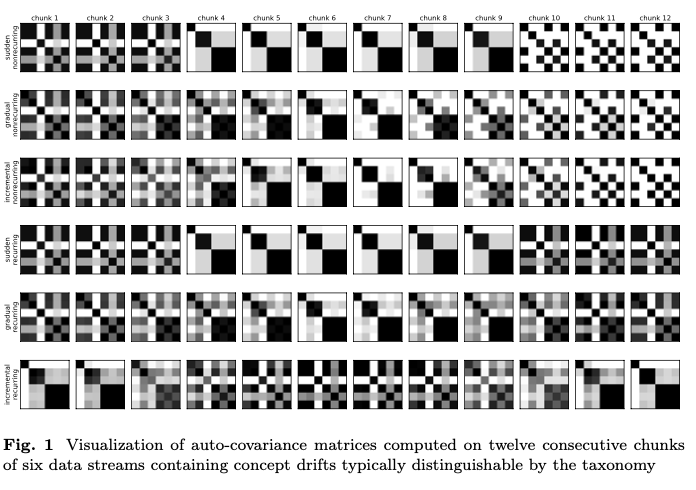
\includegraphics[width=1\textwidth, clip=true, trim=0 270 0 0]{figures/CS1}
	\caption{Wizualizacja macierzy auto-kowariancji wyznaczonych na dwunastu następujących po sobie wsadach sześciu strumieni danych zawierających dryfy koncepcji typowe dla literatury.}\label{fig:CS1}
\end{figure*}

Jak można zaobserwować, struktura zależności pomiędzy atrybutami problemu, mierzona jako ich wariancja i kros-wariancja, zmienia się proporcjonalnie do dynamiki dryfów koncepcji. W najprostszym przypadku dryfu nagłego, sygnatury koncepcji pozwalają na jednoznaczną identyfikację aktualnej interpretacji problemu. Z drugiej strony, przy dryfach inkrementalnych i gradualnych, faza przejściowa koncepcji rejestrowana jest jako płynna, stopniowa zmiana sygnatur.

Proponowana w pracy metoda \emph{Covariance-signature Concept Selector} (\textsc{cscs}) wzoruje się w swojej procedurze uczącej na takich metodach \emph{state-of-the-art}, jak \emph{Adaptive Random Forest} (\textsc{arf}), \emph{Leveraging Bagging} (\textsc{lbc}) czy \emph{Kappa Updated Ensemble} (\textsc{kue}) i również buduje zespół klasyfikatorów, ale -- w przeciwieństwie do nich -- nie integruje modeli, dokonując selekcji najbardziej odpowiedniego modelu dla aktualnie interpretowanego wsadu. Oznacza to, że inaczej niż w dotychczas stosowanych metodach, decyzja podejmowana jest zawsze przez pojedynczy model, zgodnie z paradygmatem statycznej selekcji. Co szczególnie ważne, oparcie selekcji na sygnaturach koncepcji umożliwia identyfikację koncepcji bez etykiet, a więc w obrębie procedury predykcyjnej, a tym samym, identyfikację najbardziej odpowiedniego modelu z dostępnej puli. Procedura \textsc{cscs} odrzuca standardowy paradygmat budowy zespołu, który opiera się w pozostałych metodach na zapewnieniu modeli o możliwie najwyższej jakości i różnorodności, zastępując go paradygmatem najwyższego podobieństwa pomiędzy problemem i jego predyktorem. Taka zmiana pozwala zarówno na identyfikację nowych koncepcji, jak i na selekcję modelu odpowiedniego dla aktualnego, nieoznaczonego wsadu.

Metoda \textsc{cscs} została poddana szerokiej ewaluacji eksperymentalnej, uwzględniającej zarówno osiem metod \emph{state-of-the-art} (z trzech generacji zespołowych algorytmów przetwarzania strumieni), jak i trzy kategorie scenariuszy testowych: 

\begin{itemize}
	\item Dwa z nich uwzględniają ewaluację na danych syntetycznych -- pochodzących zarówno z generatorów \textsc{moa}, jak i generatora \emph{stream-learn}
	\item Trzeci opiera się na strumieniach pół-syntetycznych, wstrzykujących dryfy do koncepcji rzeczywistych, pozwalając na ustrumieniowienie problemów stacjonarnych~\citeM{Kom22b}\marginnote{Strategia ta opisana została w osobnym artykule, przyjętym do publikacji na konferencji ESANN'22, na którą przygotowaliśmy krótki film prezentujący zasadę działania generatora strumieni.\\\noindent\url{https://youtu.be/00KEJXAQrt8}}.	
\end{itemize}

Dodatkowo, jako modele bazowe dla eksperymentów przyjęto zarówno \emph{Hoeffding Tree} (w implementacji \textsc{cvfdt}), jak i \emph{Multilayer Perceptron}. Podejście takie pozwoliło na odpowiednią analizę zachowania wszystkich rozważanych metod w problemach o różnej charakterystyce atrybutów (ilościowe, jakościowe i hybrydowe) przy różnych bazowych modelach klasyfikacji.

%Uzyskane rezultaty (Tabela~\ref{tab:CSCS}) pozwalają na identyfikację jednoznacznych trendów w przetwarzaniu. Stanowiący obecnie \emph{state-of-the-art} dziedziny algorytm \emph{Leverage Bagging Clasifier} -- zgodnie z przewidywaniami i raportami dostępnymi w literaturze -- okazuje się budować modele istotnie przewyższające konkurencję w wypadku strumieni o atrybutach jakościowych. Analogicznie jak w podobnej do niego metodzie \emph{Adaptive Random Forest}, nie stosuje się go jednak w kombinacji z innymi klasyfikatorami bazowymi niż drzewa Hoeffdinga, co utrudnia mu osiąganie wysokich rezultatów w wypadku problemów o cechach jakościowych. Wykonując tę analizę wyłącznie w oparciu o drzewa Hoeffdinga należałoby jednoznacznie przyjąć jego przewagę nad pozostałymi rozważanymi metodami rozpoznawania, ale byłoby to działanie pochopne -- pomijające ograniczenia metod drzewiastych w przetwarzaniu danych ilościowych.

Globalna analiza, uwzględniająca również perceptron wielowarstowy, pokazuje, że w wypadku wszystkich strumieni ilościowych, połączenie \emph{Multilayer Perceptron} i \textsc{cscs} wykazuje istotną przewagę statystyczną zarówno nad wszystkimi pozostałymi metodami rozpoznawania opartymi o sieci neuronowe, jak i względem modeli opartych o \emph{Hoeffding Tree}.

Podobnie prezentują się wyniki osiągnięte dla strumieni pół-syntetycznych. W wypadku niskiej wymiarowości, w których sygnatura koncepcji jest niewielka i nie uzyskuje jeszcze pełnego potencjału różnicującego, pewną przewagę nad \textsc{cscs} wykazują jeszcze modele \textsc{arf} i \textsc{lbc}. Po przekroczeniu czterech wymiarów problemu, sygnatury \textsc{cscs} pozwalają już na właściwą identyfikację i budują modele sieci neuronowych statystycznie istotnie lepsze od każdego z pozostałych testowanych rozwiązań. 

Dodatkową właściwością \textsc{cscs} jest minimalizacja narzutu obliczeniowego niezbędnego do konstrukcji modelu o dużej zdolności dyskryminacyjnej. Jak można zaobserwować na Rysunku~\ref{fig:wegiel}, proponowana przeze mnie metoda wykazuje minimalnie większą złożoność jedynie względem najstarszego i najprostszego zespołu strumieniowego -- \emph{Streaming Ensemble Algorithm}. Ponadto, model ten, kiedy oparty jest o~\emph{Multilayer Perceptron}, wykazuje o~rząd niższą złożoność obliczeniową niż bazowy model \emph{Hoeffding Tree} w problemach wielowymiarowych, prezentując się jako niezwykle skuteczne narzędzie w~przetwarzaniu wielowymiarowych strumieni danych o~charakterystyce ilościowej.

\begin{figure}[!htb]
	\centering
	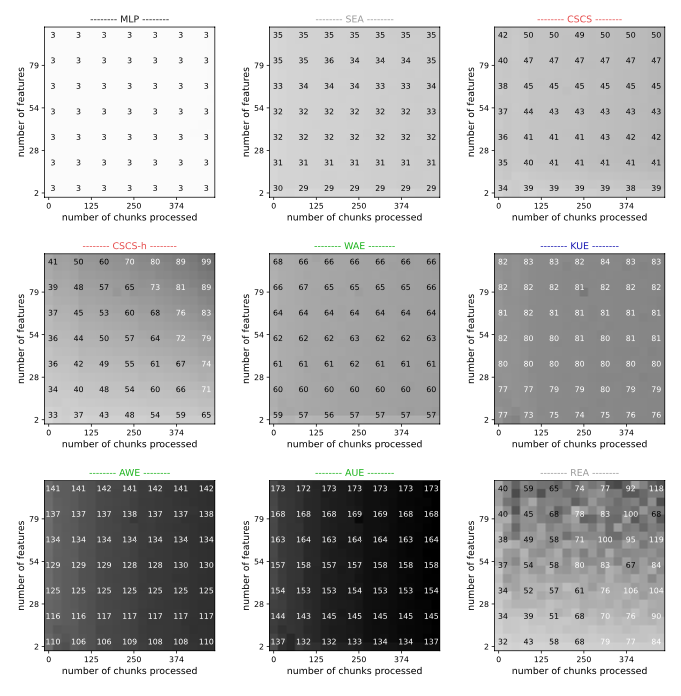
\includegraphics[width=1\textwidth, clip=true]{figures/wegiel}
	\caption{Czas (w milisekundach) wymagany do przetworzenia pojedynczego wsadu przez różne metody zespołowe wykorzystujące \temph{Multilayer Perceptron} w zależności od liczby przetworzonych wsadów i wymiarowości problemu.}\label{fig:wegiel}
\end{figure}

\vspace{1em}
\newpage
{
\color{red}
\noindent\begin{tabular}{p{\textwidth}}
	\toprule &
\end{tabular}\vspace{-1em}
}
\noindent Zagadnienie identyfikacji zmian koncepcji, przyjmując już bardziej typowe podejście wykorzystujące detektory dryfów i przebudowę modeli bez identyfikacji rozkładu, rozważałem również w pracy~\citeC[-5em]{C1}.

W pracy tej proponowany jest efektywny zespół detektorów dryfu \emph{Statistical Drift Detection Ensemble} (\textsc{sdde}), oparty na statystycznych miarach \emph{drift magnitude} oraz \emph{conditioned marginal covariate drift}, stanowiący przykład detektora agnostycznego, tj. niezależnego od odpowiedzi klasyfikatora. Należy zaznaczyć, że nie oznacza to budowy modelu nienadzorowanego, ponieważ wykorzystuje on etykiety obiektów do budowy reprezentacji wiedzy o rozkładzie klas, ale nie uzależnia swoich decyzji od zmian jakości klasyfikacji w funkcji czasu, jak robią to klasyczne detektory dryfu.

Miara \emph{drift magnitude} definiowana jest przez dystans pomiędzy koncepcjami w punktach w czasie $t$ i $u$, rozumiana jako dystans pomiędzy rozkładami atrybutów $P(X)$ w tychże

\begin{equation}
	DM_{t,u} = D(P_t(X), P_u(X)),
\end{equation}

\noindent gdzie dystans pomiędzy rozkładami estymowany jest przez metrykę Hellingera.

Druga wykorzystana miara, \emph{conditioned marginal covariance drift} definiowana jest jako ważona suma odległości pomiędzy warunkowymi rozkładami prawdopodobieństwa dla możliwych kategorii $P(X|Y)$ pomiędzy punktami w czasie $t$ i $u$. Wagi stanowią średnie prawdopodobieństwa wystąpienia obiektów danej klasy $P(Y)$ w obu punktach w~czasie

\begin{equation}
	\sigma_{t,u}^{X|Y} = \sum_{y\in Y} \Big[ \frac{P_t(y)+P_u(y)}{2} \frac{1}{2} \sum_{y\in Y} |P_t(\bar{x}|y)-P_u(\bar{x}|y)| \Big].
\end{equation}

W metodzie \textsc{sdde} miary nie są wyliczane na pełnej wymiarowości strumienia, a jedynie na jego podprzestrzeniach, czyniąc z niej rozwiązanie dedykowane strumieniom wielowymiarowym. Rozbicie problemu na podprzestrzenie nie tylko pozwala uniknąć problemów wynikających z klątwy wielowymiarowości, ale także zapewnia zespół detektorów w~miejsce pojedynczego narzędzia pomiarowego. W~jednej z wcześniejszych prac zespołu zauważyliśmy, że klasyczne metody integracji puli -- typowe dla zadania klasyfikacji -- nie przynoszą tak dobrych rezultatów w detekcji dryfu~\citeM{Woz16}, w~związku z czym dla \textsc{sdde} zaproponowana została integracja dwupoziomowa. W~ramach detektorów bazowych, zbudowanych w~obrębie tej samej podprzestrzeni), decyzja podejmowana jest na podstawie porównania aktualnych wartości metryk ze średnią harmoniczną wartości historycznych, opierając się na regule trzy-sigma. Integracja podprzestrzeni odbywa się już przez hiperparametr progu wzbudzenia, dobrany eksperymentalnie dla analizowanych strumieni. Przykład przetwarzania algorytmu \textsc{sdde} zaprezentowany został na Rysunku~\ref{fig:sdde}.

\begin{figure}[!htb]
	\centering
	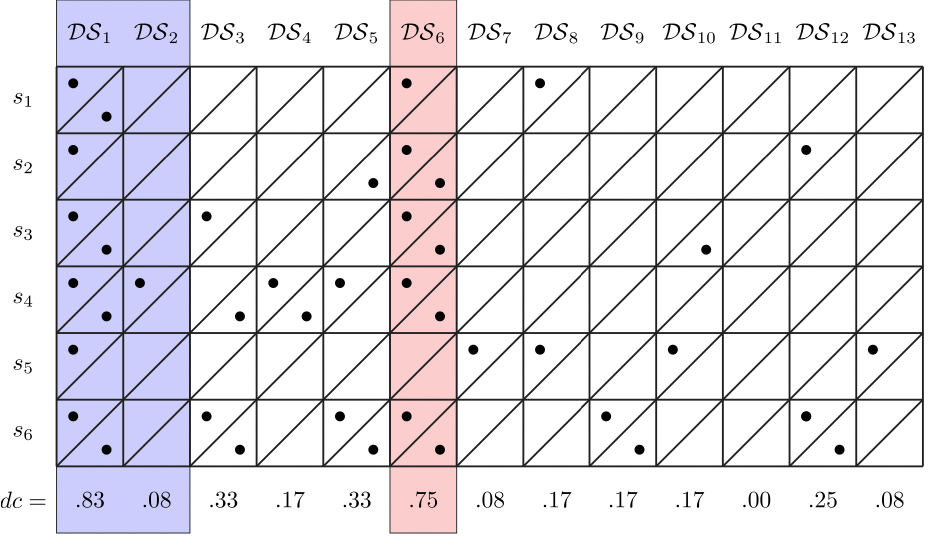
\includegraphics[width=\textwidth, clip=true]{figures/sdde}
	
\begin{enumerate}
	\item Początkowa faza przetwarzania, zaznaczona kolorem niebieskim, stanowi okres unieruchomienia wzbudzeń, w których niezależnie od odpowiedzi detektorów, zespół wskazuje na stabilność koncepcji. 
	\item Jednostkowe wzbudzenia detektorów bazowych -- oznaczone czarnymi kropkami -- nie prowadzą do przebudowania informacji o rozkładach, informując jedynie o aktualnym stanie odległości pomiędzy rozkładem pierwotnym i aktualnym.
	\item Osiągnięcie progu wzbudzenia zespołu -- zaznaczone na czerwono -- prowadzi do wyzwolenia aktualizacji modelu, zapisania informacji o~aktualnym rozkładzie w każdej podprzestrzeni i wykorzystywaniu jej jako punktu odniesienia w nadchodzących wsadach aż do momentu kolejnej detekcji dryfu.
\end{enumerate}


	\caption{Przykład przetwarzania algorytmu \emph{Statistical Drift Detection Ensemble}. Kolejne kolumny prezentują kolejne analizowane wsady, kolejne wiersze to następujące po sobie pary detektorów. Punkt oznacza wzbudzenie pojedynczego detektora, obszar niebieski -- interwał ochronny zespołu detektorów, a obszar czerwony -- wsad, w którym zespół identyfikuje dryf koncepcji. Opis procedury znajduje się w punktach poniżej ilustracji.}\label{fig:sdde}
\end{figure}

Za estymator rozkładów prawdopodobieństwa w każdym z niezbędnych elementów przyjęto jądrową estymację gęstości (\emph{Kernel Density Estimation}).

Istotnym uzupełnieniem pracy była propozycja korekty w standardowym podejściu do analizy efektywności detektorów dryfu. Jak zostało to już zauważone w literaturze, odradza się ewaluację detektorów wyłącznie w oparciu o jakość klasyfikacji, ponieważ podejście takie nie tylko utrudnia wyciąganie właściwych wniosków z badań, ale nawet promuje metody losowo przebudowujące modele co zadany interwał. Przedstawiona propozycja stanowi zbiór trzech metryk uzupełniających:

\begin{itemize}
	\item[$D_1$] -- miara najbliższego dryfu -- średnia odległość każdej detekcji od najbliższego dryfu.
	\item[$D_2$] -- miara najbliższej detekcji -- średnia odległość każdego rzeczywistego dryfu do najbliższej detekcji.
	\item[$R$] -- współczynnik dryfu do detekcji -- skalowana do zera w wartości oczekiwanej i wyznaczana z wartości bezwzględnej proporcja pomiędzy liczbą dryfów i detekcji.
\end{itemize}

Zrealizowana ewaluacja eksperymentalna pozwoliła na zweryfikowanie algorytmu \textsc{sdde} jako efektywnego narzędzia detekcji dryfu, w~szczególności w przypadkach trudnych. W~ramach oceny zwalidowano jego jakość w zestawieniu z metodami \emph{state-of-the-art} takimi jak \textsc{hddm} (w odmianach \textsc{hddm}$_A$ i \textsc{hddm}$_W$) czy \textsc{adwin}, oraz z klasycznymi detektorami \textsc{ddm} i \textsc{eddm}. Jak można zauważyć na reprezentatywnym przypadku (Rysunek~\ref{fig:sdde2}), detektor ten nie tylko pozwala na jednoznaczną identyfikację dryfu w czytelnym scenariuszu dryfu nagłego, gdzie jedynie algorytmy \textsc{hddm}$_w$ i \textsc{adwin} były zdolne do nawiązania z nim konkurencji, ale i w dryfach gradualnych, pozwalając na rozpoznanie zmian już w początkowej fazie dryfu, informując model na bieżąco o ich dynamice -- podobnie jak metoda \textsc{cscs} -- będąc czułym nie tylko na stabilne koncepcje główne, ale też na każdą z koncepcji pośrednich.

\begin{figure}[!htb]
	\centering
	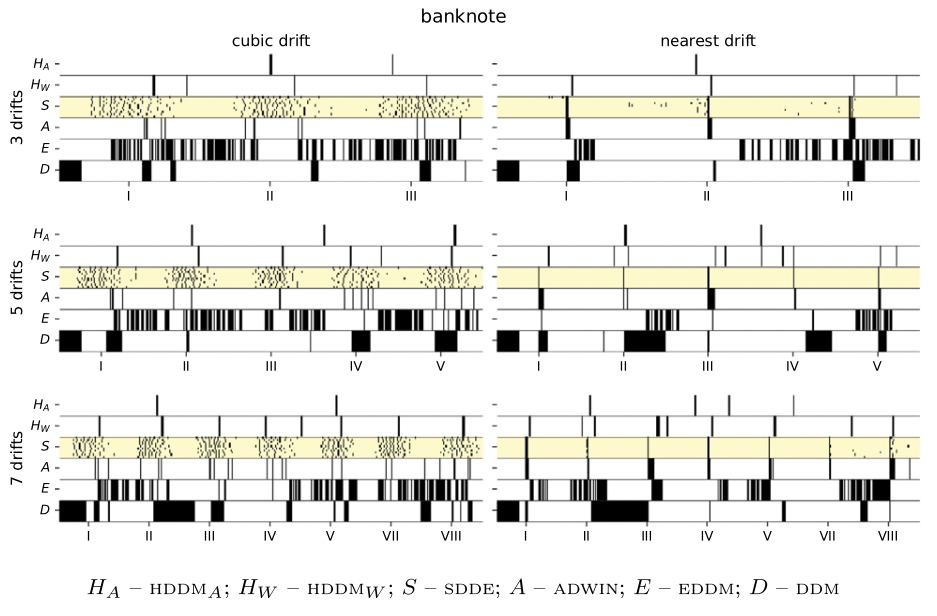
\includegraphics[width=\textwidth, clip=true, trim= 0 400 0 0]{figures/sdde2}
	\caption{Przykładowy wynik ewaluacji metody \emph{Statistical Drift Detection Ensemble} (na żółto) w scenariuszu półsyntetycznym.}\label{fig:sdde2}
\end{figure}

\subsection{Podsumowanie osiągnięcia naukowego i kierunki dalszych badań}

Prace opisane w ramach zaprezentowanego cyklu publikacji stanowią podsumowanie kolekcji metod pozwalających modelom klasyfikacji rozwiązywać szerokie spektrum problemów, w których często niemożliwe jest efektywne zastosowanie typowych rozwiązań znanych z literatury, a~nawet algorytmów \emph{state-of-the-art}. 

Koncentracja trudności, przykładowo, w wielowymiarowych strumieniach danych wykazujących zarówno dryf koncepcji, jak i dynamiczne niezbalansowanie o charakterystyce uniemożliwiającej jego funkcyjną analizę\sidenote{Strumienie niezbalansowane kategorii \textsc{ddis}}, wymaga metod specyficznych, radzących sobie z wieloma wyzwaniami równocześnie. Zaproponowany przeze mnie zbiór algorytmów stara się wychodzić tym trudnościom naprzeciw, wykazując w większości przypadków statystycznie istotnie lepsze wyniki nad rozwiązaniami znanymi z literatury, zalecanymi często do typowych problemów, dostosowanymi do ogólnych przypadków klasyfikacji danych trudnych, ale przez to też niezdolnymi do efektywnego przetwarzania w przypadkach skrajnych.

Podczas projektowania eksperymentów takiego właśnie scenariusza~\citeC{C7}, większość implementacji wykorzystywanych w badaniach trudnych strumieni danych opierała się na frameworku \textsc{moa}, stanowiącym ówczesny standard badawczy dla rozwiązań uczenia online, przeprowadzanych zgodnie z protokołem \emph{Prequential Analysis}, opierając modele na odmianach \emph{Hoeffding Tree}. Pakiet ten nie udostępniał jednak interfejsu programistycznego pozwalającego na badania z zakresu uczenia aktywnego, a więc konieczne było opracowanie dodatkowego oprogramowania pozwalającego na stosowną analizę.

Ze względu na rosnącą ówcześnie popularność pakietu \emph{scikit-learn} i~języka Python w środowisku badań nad sztuczną inteligencją, rozpocząłem prace nad nową biblioteką -- nastawioną na przetwarzanie wsadowe i ewaluację uwzględniającą ilościową naturę danych strumieniowych. Jej~pierwsza wersja rozwojowa użyta została jako podstawa do ówcześnie realizowanych badań, a stabilna wersja została opublikowana wraz z~artykułem towarzyszącym w~czasopiśmie Neurocomputing, w~styczniu 2022 roku~\citeM{Ksi22a}.

Takie podejście do badań sprawia, że zaproponowane rozwiązania nie stanowią jedynie rozważań teoretycznych, ograniczonych do odseparowanych środowisk eksperymentowania, ale w dominującej większości są dostępne dla społeczności akademickiej w formie zoptymalizowanych i~udokumentowanych implementacji wchodzących w~skład dostępnych w publicznych repozytoriach pakietów oprogramowania \emph{stream-learn}, \emph{weles} i \emph{problexity}.

\begin{itemize}
	\item \emph{Stream-learn — open-source Python library for difficult data stream batch analysis}\\%\marginnote[0em]{\noindent
\includegraphics[width=1.5cm]{WoS.png}}
	
	\url{https://github.com/w4k2/stream-learn}\\
	\url{https://stream-learn.readthedocs.io}\\
	\newpage
	
	\item \emph{Weles — Collection of pattern recognition methods and experimental tools made by ML Group of Wrocław University of Science and Technology.} \\%\marginnote[0em]{\noindent
\includegraphics[width=1.5cm]{WoS.png}}
	
	\url{https://github.com/w4k2/weles}\\
	\url{https://weles.readthedocs.io}\\

	\item \emph{Problexity — an open-source python library containing the implementation of measures describing the complexity of the classification problem.} \\%\marginnote[0em]{\noindent
\includegraphics[width=1.5cm]{WoS.png}}
	
	\url{https://github.com/w4k2/problexity}\\
	\url{https://problexity.readthedocs.io}\\	\vspace{1em}
\end{itemize}
 
 Pozwala to zarówno na replikację prezentowanych rezultatów badań, jak i dalszy ich rozwój, umożliwiający inkrementalne ulepszanie rozwiązań dedykowanych klasyfikacji danych trudnych. 
 Wśród metod, które zaproponowałem w pracach wchodzących w skład cyklu należy wymienić:

\begin{itemize}
	\item \textbf{Metodę\marginnote{\emph{dane wielowymiarowe}} zespołowej klasyfikacji obrazów nadwidmowych w oparciu o Extreme Learning Machines} -- algorytm pozwalający na wykorzystanie, szczególnie pożądanego w praktycznych aplikacjach (w~zagadnieniu rolnictwa precyzyjnego czy kontroli jakości), podejścia ręcznej inżynierii atrybutów projekcyjnych przy zastosowaniu szybko uczących się modeli neuronowych.
	\item[]\vspace{-.5em} \emph{\color{red}\footnotesize\fullcite{C10}}
	 
	\item \textbf{Genetyczną\marginnote{\emph{dane wielowymiarowe}\\\noindent\emph{dane niezbalansowane}} metodę doboru zespołu klasyfikatorów w środowisku niezbalansowanych danych wielowymiarowych} -- metodę pozwalającą na optymalizację efektywności modeli w problemach niezbalansowanych o liczności klasy mniejszościowej uniemożliwiającej syntetyczne balansowanie problemu.\\
	\item[]\vspace{-.5em} \emph{\color{red}\footnotesize\fullcite{C9}}
	
	\item \textbf{\emph{Exposer\marginnote{\emph{dane wielowymiarowe}\\\noindent\emph{dane niezbalansowane}} Classifier Ensemble}} -- zespołową metodę klasyfikatora bazowego, odporną na klątwę wielowymiarowości i niezależną od stopnia niezbalansowania problemu przy jednoczesnym zachowaniu braku zależności statystycznej względem typowych modeli rozpoznawania. 
	\item[]\vspace{-.5em} \emph{\color{red}\footnotesize\fullcite{C11}}
	
	\item \textbf{\emph{Subspace-driven\marginnote{\emph{dane wielowymiarowe}\\\noindent\emph{dane niezbalansowane}} SMOTE}} -- architekturę zespołu klasyfikatorów przesuwającą fazę przetwarzania wstępnego do -- zdatnego do krzyżowej oceny i dodatkowej kalibracji -- zbioru podprzestrzeni problemu, redukujących negatywne skutki klątwy wielowymiarowości. 
	\item[]\vspace{-.5em} \emph{\color{red}\footnotesize\fullcite{C6}}
	
	\item \textbf{\emph{Undersampled\marginnote{\emph{dane niezbalansowane}} Majority Class Ensemble}} -- architekturę zespołu klasyfikatorów dedykowaną danym silnie niezbalansowanym, pozwalającą na pełne wykorzystanie dostępnych obiektów problemu, bez konieczności wprowadzania do przetwarzania obiektów syntetycznych.
	\item[]\vspace{-.5em} \emph{\color{red}\footnotesize\fullcite{C8}}
	
	\item \textbf{Metodę\marginnote{\emph{strumienie danych}} aktywnego przetwarzania strumieni danych opartą o~\emph{Relative Support Function Difference}} -- pozwalającą na racjonalizację kosztu pozyskiwania stronniczości eksperckiej w~problemach o~zmiennym prawdopodobieństwie \emph{a posteriori}.
	\item[]\vspace{-.5em} \emph{\footnotesize\color{red}\fullcite{C7}}
	
	\item \textbf{\emph{Prior\marginnote{\emph{dane niezbalansowane}\\\noindent\emph{strumienie danych}} Imbalance Compensation}} -- agnostyczną procedurę pozwalającą na zwiększenie mocy dyskryminacyjnej modeli klasyfikacji w strumieniach niezbalansowanych bez konieczności stosowania przetwarzania wstępnego, metod wbudowanych ani hybrydowych.  
	\item[]\vspace{-.5em} \emph{\footnotesize\color{red}\fullcite{C4}}
	
	\item \textbf{\emph{Dynamic\marginnote{\emph{dane niezbalansowane}\\\noindent\emph{strumienie danych}} Statistical Concept Analysis}} -- rozwinięcie metody \textsc{pic} o~efektywny estymator prawdopodobieństwa \emph{a priori}, zdolny do osiągania wysokiej efektywności nawet w skrajnych przypadkach strumieni o niezbalansowaniu dyskretnie-dynamicznym.
	\item[]\vspace{-.5em} \emph{\footnotesize\color{red}\fullcite{C3}}
	
	\item \textbf{\emph{Covariance-signature\marginnote{\emph{dane wielowymiarowe}\\\noindent\emph{dane niezbalansowane}\\\noindent\emph{strumienie danych}} Concept Selector}} -- zespołową metodę klasyfikacji trudnych strumieni danych o cechach ilościowych, dedykowaną przetwarzaniu z wykorzystaniem modeli sieci neuronowych.
	\item[]\vspace{-.5em} \emph{\footnotesize\color{red}\fullcite{C2}}
	
	\item \textbf{\emph{Statistical\marginnote{\emph{strumienie danych}} Drift Detection Ensemble}} -- zespołowy detektor dryfu dedykowany rozpoznawaniu zmian w rozkładach \emph{a posteriori} dla strumieni wielowymiarowych, stanowiący metodę agnostyczną -- niezależną od wykorzystywanego modelu klasyfikacji.
	\item[]\vspace{-.5em} \emph{\footnotesize\color{red}\fullcite{C1}}
	 
\end{itemize}


\noindent Oprócz tematyki zawartej w prezentowanym cyklu moje zainteresowania naukowe dotyczą również innych tematów sztucznej inteligencji. Zagadnienie detekcji źródeł dezinformacji i klasyfikacji \emph{fake news}, który poruszyłem tu w kontekście przetwarzania strumieniowego, rozwijam w kolejnych pracach analitycznych, w których znajdują się zarówno propozycje nowych algorytmów, jak i najaktualniejszy obecnie artykuł przeglądowy~\citeM[-4em]{Cho21} stanowiący zbiór punktów wyjścia dla prac prowadzonych w ramach kierowanego przeze mnie projektu \textsc{swarog}\footnote{Na tropie fake newsów, czyli projekt \textsc{swarog}\\\noindent\url{https://wit.pwr.edu.pl/aktualnosci/na-tropie-fake-newsow-\\-czyli-projekt-swarog-5.html}}.


Zagadnienie przetwarzania strumieni danych analizuję również w~kontekście zespołowych detektorów dryfu, strumieni niezbalansowanych skrajnie, modyfikacji standardowych metryk ważenia zespołów klasyfikatorów, dalszych prac nad uczeniem aktywnym czy oceny potencjału balansowania strumieni. 

Dane niezbalansowane analizuję też nadal w ich stacjonarnej odmianie, zarówno dla danych sygnałowych jak i tabelarycznych, uwzględniając tu zarówno wątek integracji geometrycznej~\citeM{Ksi21k} jak i potencjału algorytmów genetycznych w dywersyfikacji zespołów. Podobnie, rozwijam też wątek przetwarzania danych wielowymiarowych, zarówno w~ujęciu tabelarycznym, jak i sygnałowym.

Ponadto, w swoich badaniach przykładam szczególną wagę do poprawności protokolarnej, o czym świadczyć może moje współautorstwo w pracy przeglądowej przedstawiającej dobre praktyki projektowania rzetelnych eksperymentów~\citeM[-2em]{Sta21}. Opisane przedsięwzięcie stanowi zarówno odpowiedź na aktualne i podlegające intensywnym badaniom problemy, jak i zbiór stabilnych rozwiązań, możliwych do zastosowania i~stosowanych w rzeczywistych problemach.

\newthought{Wykorzystana literatura pomocnicza}

{\footnotesize
\begin{fullwidth}
\begin{itemize}
	\item[[Z1]] \fullcite{Z1}
	\item[[Z2]] \fullcite{Z2}
	\item[[Z3]] \fullcite{Z3}
	\item[[Z4]] \fullcite{Z4}
	\item[[Z5]] \fullcite{Z5}
	\item[[Z6]] \fullcite{Z6}
	\item[[Z7]] \fullcite{Z7}
	\item[[Z8]] \fullcite{Z8}
	\item[[Z9]] \fullcite{Z9}
	\item[[Z10]] \fullcite{Z10}
	\item[[Z11]] \fullcite{Z11}
	\item[[Z12]] \fullcite{Z12}
	\item[[Z13]] \fullcite{Z13}
	\item[[Z14]] \fullcite{Z14}
	\item[[Z15]] \fullcite{Z15}
	\item[[Z16]] \fullcite{Z16}
	\item[[Z17]] \fullcite{Z17}
	\item[[Z18]] \fullcite{Z18}
	\item[[Z19]] \fullcite{Z19}
	\item[[Z20]] \fullcite{Z20}
	\item[[Z21]] \fullcite{Z21}
	\item[[Z22]] \fullcite{Z22}
	\item[[Z23]] \fullcite{Z23}
	\item[[Z24]] \fullcite{Z24}
	\item[[Z25]] \fullcite{Z25}
	\item[[Z25]] \fullcite{Z26}
\end{itemize}
\end{fullwidth}
}
\section{Informacja o wykazywaniu się istotną aktywnością naukową albo artystyczną realizowaną w więcej niż jednej uczelni, instytucji naukowej lub instytucji kultury, w szczególności zagranicznej}

%Pracę naukową rozpocząłem na ostatnim roku studiów magisterskich, realizując projekt przewidywania występowania sztormów na Morzu Bałtyckim, w oparciu o samodzielnie skonstruowany strumień serii czasowej dla zadanej, interpolowanej siatki punktów próbkowania stanu pogody zbudowanej na podstawie odczytów stacji meteorologicznych. W 2013 roku rozpocząłem studia doktoranckie na Wydziale Elektroniki, Politechniki Wrocławskiej, skupiając się na tematyce przetwarzania wielowymiarowych sygnałów cyfrowych w kontekście ich segmentacji, klasteryzacji i klasyfikacji. W 2015 roku uzyskałem zatrudnienie na stanowisku asystenta naukowo-dydaktycznego w Katedrze Systemów i Sieci Komputerowych, gdzie też w 2017 roku złożyłem pracę doktorską w tematyce reprezentacji i analizy danych wielowymiarowych. Stopień doktora nauk technicznych w dyscyplinie informatyka (z wyróżnieniem) uzyskałem zgodnie z uchwałą Rady Wydziału Elektroniki Politechniki Wrocławskiej, 21 czerwca 2017 roku. 

Po zatrudnieniu na stanowisku adiunkta, w październiku 2017 roku, zmieniłem główne zainteresowania badawcze, skupiając się na klasyfikacji danych niezbalansowanych i przetwarzaniu strumieni danych, ze szczególnym uwzględnieniem wsadowego paradygmatu przetwarzania}. 

Dalsze prace starałem się realizować w sposób, który pozwala na retencję wiedzy i stosowanych metod, przykładając szczególną wagę do replikowalności eksperymentów i otwartości oprogramowania opracowywanego w ramach bieżących prac \emph{Katedry Systemów i Sieci Komputerowych}\sidenote[][-5em]{Większość badań pracowników Katedry z ostatnich pięciu lat publikowana jest również jako oprogramowanie eksperymentalne dostępne na prowadzonym przeze mnie profilu organizacji na GitHub:\\\noindent\url{https://github.com/w4k2}}. Silną współpracę w tym okresie prowadziłem zarówno z~doktorantami zatrudnionymi w~jednostce, z których dwóch uzyskało w~tym roku stopień doktora, jak i z~pracownikami innych zespołów badawczych \emph{Politechniki Wrocławskiej}. 

Szczególnie istotny jest dla mnie aspekt multidyscyplinarności badań, która pozwala na odnajdywanie szerszych zastosowań  proponowanych przeze mnie metod. Wyraża się ona, między innymi, w ścisłej współpracy z \emph{Zespołem Sieci Komputerowych}, gdzie wspólnie z badaczami z~\emph{Instytutu Łączności\sidenote[][-7em]{\\\noindent\emph{Instytut Łączności -- Państwowy Instytut Badawczy}\\\noindent\url{https://itl.waw.pl/}}} budujemy algorytmy wspomagające optymalizację kognitywnych sieci optycznych z wykorzystaniem modeli regresji~\citeM[-4.25em]{Ksi20s}. Wykorzystując zdobytą wcześniej wiedzę z zakresu przetwarzania cyfrowych sygnałów wielowymiarowych, angażuję się także w~badania z~zakresu bioinformatyki, gdzie wspólnie z~pracownikami \emph{Katedry Inżynierii Biomedycznej} oraz \emph{School of Optometry and Vision Science}\sidenote[][-1em]{\\\noindent\emph{School of Optometry and Vision Science},\\\noindent Brisbane, Australia} i~\emph{Uniwersytetu Medycznego we Wrocławiu} analizujemy potencjał metod uczenia maszyn w zagadnieniu wczesnej detekcji jaskry~\citeM{Sul21b}.

Po zakończeniu doktoratu nawiązałem też silną współpracę z pracownikami \emph{Zakładu Systemów Teleinformatycznych Wydziału Telekomunikacji, Informatyki i Elektrotechniki, Politechniki Bydgoskiej}. W ramach współpracy zrealizowaliśmy międzynarodowy projekt \emph{SocialTruth}, finansowany ze środków programu \emph{EU Horizon 2020}, prowadzony w konsorcjum z 11 państw \emph{Unii Europejskiej}\sidenote{\emph{SocialTruth}\\\url{http://socialtruth.eu}}. W latach 2019--2021 byłem zatrudniony w tym projekcie, publikując cztery prace naukowe, a dwie kolejne oczekują obecnie na recenzje.

Osiągnięcia poczynione w toku realizacji projektu \emph{SocialTruth} pozwoliły nam również opracować wniosek projektowy w ramach programu \textsc{infostrateg i}\sidenote{\url{https://www.gov.pl/web/ncbr/infostrateg-i-konkurs}}, poświęcony zagadnieniu klasyfikacji fake news w~języku polskim, który uzyskał maksymalną punktację \textsc{ncb}i\textsc{r}, zdobył finansowanie na poziomie ponad ośmiu milionów złotych~\sidenote{\emph{System Wykrywania Dezinformacji Metodami Sztucznej Inteligencji
}\\\noindent\url{https://www.kssk.pwr.edu.pl/projects/swarog}} i w którym od grudnia 2021 roku pełnię rolę kierownika badawczo-rozwojowego. Projekt \emph{SWAROG} realizowany jest w konsorcjum z \emph{Politechniką Bydgoską} i przedsiębiorstwem \emph{Matic SA}.

Wspólna praca w międzynarodowym konsorcjum -- m. in. podczas spotkań projektowych w Paryżu i Rzymie -- pozwoliła mi także na nawiązanie współpracy z innymi europejskimi ośrodkami w zakresie wspólnych publikacji. Wspólne badania z zakresu klasyfikacji \emph{fake news} z zespołami \emph{National Technical University of Athens\sidenote[][-3em]{\\\noindent\emph{National Technical University of Athens},\\\noindent Ateny, Grecja}} i \emph{Universidad de Burgos\sidenote{\\\noindent\emph{Universidad de Burgos},\\\noindent Burgos, Hiszpania}} doprowadziły do opracowania pracy przeglądowej z zakresu metod detekcji źródeł dezinformacji~\citeM[.5em]{Cho21}. W ubiegłym roku pełniłem też rolę członka komisji doktorskiej przewodu Nuno Basutro z \emph{Universidad de Burgos}, który podczas swoich studiów doktoranckich odbył staż na \emph{Politechnice Wrocławskiej}.

Wymiana doświadczeń z zakresu projektowania eksperymentów rozpoznawania wzorców -- ze szczególnym uwzględnieniem metod statystycznego testowania hipotez -- podjęta wspólnie z zespołami \emph{Politechniki Śląskiej} i \emph{University of Granada}\sidenote{\\\noindent\emph{University of Granada},\\\noindent Granada, Hiszpania} pozwoliły z kolei na opracowanie pracy przeglądowej dotyczącej dobrych praktyk eksperymentowania z~algorytmami klasyfikacji~\citeM{Sta21}. Wprowadzamy tym zarówno zbiór wytycznych poprawnej ewaluacji, jak i prezentujemy praktyczne przykłady powszechnych, acz błędnych strategii oceny, które często prowadzą do uzyskiwania niejednoznacznych wniosków z badań.\vspace{1em}

\noindent W toku swojej pracy naukowej odbyłem także trzy krótko i średnioterminowe staże naukowe:

\begin{itemize}
	\item Dwa staże naukowe zrealizowałem w ramach współpracy z \emph{Universidad del Pais Vasco}\sidenote[][-2em]{\\\noindent\emph{Universidad del Pais Vasco}\\\noindent San Sebastian, Hiszpania}, które zakończyły się nawiązaniem trwałej współpracy badawczej z zespołem \emph{Group Faculty of Informatics} kierowanym przez profesora Manuela Granę~\citeM[-1.5em]{Ksi17p}. Współpraca ta wyraża się zarówno we wspólnych pracach badawczych, jak i w wymianie doświadczeń projektowych, której podsumowaniem może być wykład, który wygłosiłem na zaproszenie podczas konferencji \emph{CybSPEED}'22. Współpraca nawiązana na wczesnym etapie pracy badawczej z \emph{Universidad del Pais Vasco} była też bardzo ważnym czynnikiem w toku realizacji mojego doktoratu, ponieważ to podczas stażu Borja Ayerdi z zespołu prof. Manuela Grany realizowałem swoje pierwsze badania z zakresu przetwarzania obrazów nadwidmowych. 
	
	\item Trzeci staż naukowy zrealizowałem w \emph{Virginia Commonwealth University}\sidenote[][-9.5em]{\\\noindent\emph{Virginia Commonwealth University}\\\noindent Richmond, VA, USA}, co pozwoliło mi na rozwinięcie wstępnych koncepcji badań z zakresu klasyfikacji danych trudnych~\citeC[-0em]{C10}. W ramach rozwijania zakresu współpracy analizujemy aktualnie tematykę \emph{wyjaśnialnej sztucznej inteligencji} (ang. \emph{explainable AI}) dla zagadnień przetwarzania strumieni danych oraz homogeniczne metody dywersyfikacji puli klasyfikatorów oparte o rozkłady niejednostajne.

\end{itemize}
 

\section{Informacja o osiągnięciach dydaktycznych, organizacyjnych oraz popularyzujących naukę lub sztukę}

Podczas dziewięciu lat pracy naukowo-dydaktycznej prowadziłem dziewiętnaście kursów dla studentów kierunków \emph{Informatyka}, \emph{Informatyka Techniczna} i \emph{Teleinformatyka}, w siedmiu z nich będąc głównym wykładowcą i autorem materiałów dydaktycznych: 

\begin{enumerate}
	\item Metody sztucznej inteligencji%\marginnote[-.5em]{\emph{(laboratorium, \textbf{wykład}, projekt)}},\vspace{1em}
	\item Methods of Computational Intelligence and Decision Making,%\marginnote[-.5em]{\emph{(laboratorium, projekt, \textbf{wykład})}}\vspace{1em}
	\item Obrazowanie biomedyczne,%\marginnote[-.5em]{\emph{(laboratorium, seminarium, \textbf{wykład})}},\vspace{1em}
	\item Przetwarzanie sygnałów wielowymiarowych,%\marginnote[-.5em]{\emph{(\textbf{wykład}, laboratorium)}},\vspace{1em}
	\item Projektowanie systemów internetowych i mobilnych,%\marginnote[-.5em]{\emph{(projekt, seminarium, \textbf{wykład})}} \vspace{1em}
	\item Projektowanie telemedycznych systemów internetowych i mobilnych,%\marginnote{\emph{(laboratorium, \textbf{wykład})}}\vspace{1em}
	\item Aplikacje mobilne.%\marginnote{\emph{(laboratorium, \textbf{wykład})}}.
\end{enumerate}

Angażuję się również w opracowywanie materiałów dydaktycznych dla studentów, uczniów oraz nauczycieli, promocję nauki przez studenckie warsztaty naukowe i współpracę z kołami naukowymi oraz promocję uczelni przez organizację \emph{hackathonów}:

\begin{itemize}
	\item Przygotowałem materiały multimedialne do nauki sztucznej inteligencji oraz serię materiałów wideo dla projektu \emph{Centrum Mistrzostwa Informatycznego}\sidenote[][-2em]{\emph{Centrum Mistrzostwa Informatycznego}\\\noindent\url{https://cmi.edu.pl}}. 
	\item Współorganizowałem kilka edycji studenckich warsztatów naukowych \emph{International Students Workshop}\sidenote[][-1.5em]{\emph{International Students Workshop}\\\noindent\url{http://sisk.kssk.pwr.edu.pl/isw/}} (2015-2019).
	\item Opiekuję się pracami badawczymi studentów w ramach działającego przy \emph{Katedrze Systemów i Sieci Komputerowych}, \emph{Koła Naukowego Systemów i Sieci Komputerowych} oraz założonego w zeszłym roku \emph{Koła Uczenia Maszyn}. 
	\item Byłem pomysłodawcą i jednym z głównych organizatorów \emph{hackathonu} \emph{JellyPizzaHack}\sidenote[][-1.5em]{\emph{JellyPizzaHack}\\\noindent\url{https://invest-in-wroclaw.pl/piwnica-dynamicznie-alokowana}}, zorganizowanego we współpracy z \emph{Credit Suisse} (16.12.2016).
\end{itemize}

Aktywnie uczestniczę także w opracowywaniu kart przedmiotów, będąc opiekunem  czterech kursów:

\begin{itemize}
	\item Projektowanie systemów informatyki medycznej,% (INES00123),
	\item Przetwarzanie sygnałów wielowymiarowych,% (INEU00127),
	\item Metody przetwarzania języka naturalnego oraz wyszukiwanie,% (INEU00129),
	\item Uczenie Maszyn.% (INEA00236).
\end{itemize}

Ponadto, od pięciu lat pełnię rolę sekretarza komisji dyplomowej specjalności \emph{Advanced Informatics and Control}, prowadzonej w języku angielskim. W tym czasie byłem także promotorem 43 prac magisterskich i 37 prac inżynierskich. Sześcioro z moich dyplomantów aktualnie realizuje swoje prace doktorskie na \emph{Politechnice Wrocławskiej}, a z pięciorgiem z nich miałem przyjemność pracować przy ich pierwszych publikacjach konferencyjnych lub publikacjach w czasopismach. Poniżej prezentuję wybraną tematykę prowadzonych prac magisterskich na przykładzie obecnych doktorantów, odnosząc się także do wspólnych prac badawczych:

\begin{itemize}
	\item Prior Probability Estimation in Dynamically Imbalanced Data Streams, 2022,~\citeC[-3em]{C3}\\\emph{mgr inż. Joanna Komorniczak}\vspace{7em}
	\item Feature extraction using n-gram methods for the purpose of ensemble classification of disinformation sources, 2021,~\citeM[-1.5em]{Bor22a}\\\emph{mgr inż. Weronika Borek-Marciniec -- pełnię rolę promotora pomocniczego}\vspace{2em}
	\item Wykorzystanie uczenia zespołowego w klasyfikacji binarnej niezbalansowanych strumieni danych, 2020,~\citeM[-1.5em]{Weg20}\\\emph{mgr inż. Weronika Węgier}\vspace{3em}
	\item Analiza efektywności zastosowania sieci rekurencyjnych w zadaniu klasyfikacji, 2019,~\citeM[-1.5em]{Koz19}\\\emph{mgr inż. Jędrzej Kozal},\vspace{3em}
	\item Analiza efektywności odmian algorytmu \textsc{smote} w balansowaniu strumieni danych, 2019,~\citeM[-1.5em]{Gul19}\\\emph{mgr inż. Bogdan Gulowaty},\vspace{3em}
	\item Zadanie uczenia nienadzorowanego w kontekście obrazowania nadwidmowego, 2018,~\citeM[-1.5em]{Sul21}\\\emph{mgr inż. Dominika Sułot}\vspace{3.5em}
\end{itemize}

Aktywnie udzielam się również w organizacji konferencji i warsztatów naukowych poświęconych zagadnieniom klasyfikacj danych trudnych, wśród których chciałbym wymienić:

\begin{itemize}
    \item \marginnote[1em]{\url{https://www.iccs-meeting.org/iccs2021/}}Organizację sesji specjalnej “\emph{Classifier Learning from Difficult Data}” na konferencji \emph{International Conference on Computational Science} (\textsc{iccs})\\
    	16–18 czerwca 2021, Kraków, Polska. Zasięg międzynarodowy.
    \item \marginnote[1em]{\url{https://www.iccs-meeting.org/iccs2020/}}Organizację sesji specjalnej “\emph{Classifier Learning from Difficult Data}” na konferencji \emph{International Conference on Computational Science} (\textsc{iccs})\\
    	3–5 czerwca 2020, Amsterdam, Holandia. Zasięg międzynarodowy.
    \item \marginnote[1em]{\url{http://www.confercare.manchester.ac.uk/events/ideal2019/sessions/}} Organizację sesji specjalnej “\emph{Machine Learning Algorithms for Hard Problems}“ na konferencji \emph{20th International Conference on Intelligent Data Engineering and Automated Learning} (\textsc{ideal})\\
    	14–16 listopada 2019, Manchester, Anglia. Zasięg międzynarodowy.
    \item \marginnote[1em]{\url{https://www.iccs-meeting.org/iccs2019/}}Organizację sesji specjalnej “\emph{Classifier Learning from Difficult Data}” na konferencji \emph{International Conference on Computational Science} (\textsc{iccs})\\
    	12–14 czerwca 2019, Faro, Portugalia. Zasięg międzynarodowy.
    \item \marginnote[1em]{\url{http://pp-rai.pwr.edu.pl/}}Organizację konferencji \emph{Polskie Porozumienie na rzecz Rozwoju Sztucznej Inteligencji},\\
    	16–18 października 2019, Wrocław, Polska. Zasięg krajowy.
    \item \marginnote[1em]{\url{http://cores.pwr.wroc.pl}}Organizację konferencji \emph{The 9 International Conference on Computer Recognition Systems} \textsc{cores},\\
    	Wrocław, Polska. Zasięg międzynarodowy
\end{itemize}

Wielokrotnie udzielałem się także w działaniach mających na celu zwiększenie świadomości społecznej z zakresu ryzyka związanego z~dezinformacją i~potencjału metod sztucznej inteligencji w~walce z~nią. Należy tu wymienić:

\begin{itemize}
    \item uczestnictwo w roli eksperta w debacie “\emph{Szczepionka na kłamstwo.}” organizowanej przez \emph{Fundację na rzecz Nauki Polskiej} w ramach cyklu „\emph{Ufajmy nauce}” (21.04.2022r.),
    \item[] \url{https://www.fnp.org.pl/debata-ekspertow-szczepionka-na-klamstwo}
    \item[] \url{https://www.youtube.com/watch?v=O75LsK0M4D4} 
    \item wygłoszenie prelekcji pod tytułem 
    \item[] \emph{Wykorzystanie sztucznej inteligencji w walce z dezinformacją} 
    \item[] w ramach seminarium "\emph{Sztuczna inteligencja w rozwoju miast i obszarów metropolitarnych}" organizowanego przez \emph{Wrocławskie Centrum Akademickie} pod patronatem \emph{World Urban Forum} (9.03.2022r.),
    \item[] \url{https://metropolie.pl/artykul/seminarium-sztuczna-inteligencja-dla-} \url{rozwoju-miast-i-obszarow-metropolitalnych}
    \item[] \url{https://vimeo.com/685793217}
    \item wykład w ramach seminarium “\emph{Machine Learning to Combat Fake News and Media Manipulation}” organizowanego przez Elsevier w ramach cyklu webinarów (20.04.2022r.).
    \item[] \url{https://www.workcast.com/register?cpak=7948916184707381}
    \item wywiady radiowe dotyczące detekcji źródeł dezinformacji:
    \begin{itemize}
	    \item[] \emph{Radio RAM\\Politechnika Wrocławska pracuje nad systemem wykrywającym fake newsy}
	    \item[] \url{https://www.radiowroclaw.pl/articles/view/110758/Politechnika-} \url{Wroclawska-pracuje-nad-systemem-wykrywajacym-fake-newsy} 
	\end{itemize}
\end{itemize}

W ostatnich latach przeprowadziłem również trzy wykłady na zaproszenie, dotyczące tematyki klasyfikacji danych trudnych oraz detekcji źródeł dezinformacji:

\begin{itemize}
    \item Keynote podczas sesji specjalnej CLDD w ramach konferencji International Conference on Computational Science.\\\vspace{.5em}
    {\large Chosen Challenges of Imbalanced Data Stream Classification}\\
    16 czerwca 2021\\
    \url{https://www.iccs-meeting.org/iccs2021/}
    \item Wykład na zaproszenie:\\\vspace{.5em}
    {\large Research practices in data stream analysis and imbalanced data classification.}\\
    22 czerwca 2020, Amity School of Engineering and Technology, Noida, Indie,
    \item Wykład w ramach Elsevier Webinar Machine Learning to combat Fake News and Media Manipulation.\\\vspace{.5em}
    {\large Using machine learning as the weapon against the disinformation}\\
    20 kwietnia 2021\\
    \url{https://www.workcast.com/register?cpak=7948916184707381}
\end{itemize}

\section{Dane bibliometryczne}


\subsection{Prace autorstwa Pawła Ksieniewicza spoza cyklu}
{\large
\begin{itemize}
	\item[[Ksi22a]] \fullcite{Ksi22a}
	\item[[Ksi22y]] \fullcite{Ksi22y}
	\item[[Ksi22z]] \fullcite{Ksi22z}
	\item[[Bor22a]] \fullcite{Bor22a}
	\item[[Gos22]] \fullcite{Gos22}
	\item[[Kom22]] \fullcite{Kom22}
	\item[[Kom22c]] \fullcite{Kom22c}
	\item[[Kom22b]] \fullcite{Kom22b}
	\item[[Kom22p]] \fullcite{Kom22p}
	\item[[Woj22]] \fullcite{Woj22}
	
	\item[[Ksi21k]] \fullcite{Ksi21k}
	\item[[Cho21]] \fullcite{Cho21}
	\item[[Sta21]] \fullcite{Sta21}
	\item[[Sul21]] \fullcite{Sul21}
	\item[[Sul21b]] \fullcite{Sul21b}
	
	\item[[Ksi20s]] \fullcite{Ksi20s}
	\item[[Ksi20b]] \fullcite{Ksi20b}
	\item[[Ksi20e]] \fullcite{Ksi20e}
	\item[[Klin20]] \fullcite{Klin20}
	\item[[Kul20]] \fullcite{Kul20}
	\item[[Weg20]] \fullcite{Weg20}
	\item[[Zyb20a]] \fullcite{Zyb20a}
	
	\item[[Ksi19f]] \fullcite{Ksi19f}
	\item[[Gul19]] \fullcite{Gul19}
	\item[[Kli19]] \fullcite{Kli19}
	\item[[Koz19]] \fullcite{Koz19}
	\item[[Zyb19]] \fullcite{Zyb19}
	
	\item[[Ksi18e]] \fullcite{Ksi18e}
	\item[[Ksi18c]] \fullcite{Ksi18c}
	\item[[Lap18]] \fullcite{Lap18}
	
	\item[[Ksi17p]] \fullcite{Ksi17p}
\end{itemize}}

\subsection{Prace autorstwa Pawła Ksieniewicza przed uzyskaniem stopnia naukowego doktora inżyniera}
{\large
\begin{itemize}
	\item[[Ksi16a]] \fullcite{Ksi16a}
	\item[[Ksi16b]] \fullcite{Ksi16b}
	\item[[Ksi16m]] \fullcite{Ksi16m}
	\item[[Woz16]] \fullcite{Woz16}
	\item[[Woz16b]] \fullcite{Woz16b}
	\item[[Woz16c]] \fullcite{Woz16c}
	\item[[Woz16d]] \fullcite{Woz16d}

	\item[[Ksi15a]] \fullcite{Ksi15a}

	\item[[Ksi14a]] \fullcite{Ksi14a}
	\item[[Jac14]] \fullcite{Jac14}
	\item[[Kra14a]] \fullcite{Kra14a}
	\item[[Kra14b]] \fullcite{Kra14b}
\end{itemize}}


\vfill\noindent\hspace{.75\textwidth}\begin{minipage}{15em}
\begin{center}
	\hbox to 5cm{\leaders\hbox to 3pt{\hss . \hss}\hfil}

	(podpis wnioskodawcy)
\end{center}
\end{minipage}


\begin{fullwidth}

\chapter{Wykaz osiągnięć naukowych albo artystycznych, stanowiących znaczny wkład w rozwój określonej dyscypliny}

	
\section{INFORMACJA O OSIĄGNIĘCIACH NAUKOWYCH ALBO ARTYSTYCZNYCH O KTÓRYCH MOWA W ART. 219 UST. 1. PKT 2 USTAWY}

\subsection{Monografia naukowa}
---

\subsection{\textbf{Cykl powiązanych tematycznie artykułów naukowych, zgodnie z art. 219 ust. 1. pkt 2b Ustawy; pt:}}

\vspace{1em}
\begin{center}
	\LARGE
	\textbf{Projektowanie algorytmów rozpoznawania wzorców dla~zadania klasyfikacji trudnych danych}
\end{center}\vspace{1em}

\noindent Wszystkie publikacje pochodzą z okresu po uzyskaniu stopnia doktora. Informacje dot. liczby punktów MEiN, współczynnika IF oraz liczby cytowań  oddają \textbf{stan na dzień 27. sierpnia 2022 r.} zgodnie z bazami publikacji naukowych:

\begin{itemize}
	\item[\textsc{WoS}] \emph{Web of Science}
	\url{https://www.webofscience.com/wos/author/record/1886494}	
	\item[\textsc{Sco}] \emph{Scopus}
	\url{https://www.scopus.com/authid/detail.uri?authorId=56206176100}
	\item[\textsc{GSc}] \emph{Google Scholar}	
	\url{https://scholar.google.com/citations?user=YSM30D8AAAAJ}
\end{itemize}

\newpage

\end{fullwidth}

%
% C1
%
\marginnote[1em]{
% MARGIN TAB
\color{red}
\begin{tabular}{rccc}
\toprule
& \textsc{WoS} & \textsc{Sco} & \textsc{GSc}\\
l. cytowań & --- & --- & --- \\\\
\multicolumn{3}{r}{\color{black}\emph{Szacowany udział}} & \color{black}70\%\\
\multicolumn{3}{r}{\color{black}\emph{Impact Factor}} & \color{black}8.139\\
\multicolumn{3}{r}{\color{black}\emph{l. punktów \textsc{me}i\textsc{n}}} & \color{black}200\\\\

%\multicolumn{4}{r}{
\includegraphics[width=1.5cm]{WoS.png}}
\end{tabular}

% BASE TAB
}\noindent\begin{tabular}{lllll@{}}
\toprule
\color{red}[C1] & \multicolumn{4}{p{28em}}{\fullcite{C1}} \\
 & \multicolumn{4}{p{30em}}{
 {\footnotesize\textsc{CRediT}}: 
 \mybox{Conceptualization} \mybox{Software} \mybox{Validation} \mybox{Investigation} \mybox{Writing - Original Draft} \mybox{Writing - Review \& Editing} \mybox{Visualization} \mybox{Supervision}}\\

%\\\\\bottomrule
\end{tabular}
\vspace{.5em}

%
% C2
%
\marginnote[1em]{
% MARGIN TAB
\color{red}
\begin{tabular}{rccc}
\toprule
& \textsc{WoS} & \textsc{Sco} & \textsc{GSc}\\
l. cytowań & --- & --- & --- \\\\
\multicolumn{3}{r}{\color{black}\emph{Szacowany udział}} & \color{black}100\%\\
\multicolumn{3}{r}{\color{black}\emph{Impact Factor}} & \color{black}5.086\\
\multicolumn{3}{r}{\color{black}\emph{l. punktów \textsc{me}i\textsc{n}}} & \color{black} 70\\\\

%\multicolumn{4}{r}{
\includegraphics[width=1.5cm]{WoS.png}}

\end{tabular}
% BASE TAB
}\noindent\begin{tabular}{lllll@{}}
\toprule
\color{red}[C2] & \multicolumn{4}{p{28em}}{\fullcite{C2}}  \\
 & \multicolumn{4}{p{30em}}{
 {\footnotesize\textsc{CRediT}}: 
 \mybox{Conceptualization} \mybox{Methodology} \mybox{Software} \mybox{Validation} \mybox{Formal Analysis} \mybox{Investigation} \mybox{Resources} \mybox{Data Curation} \mybox{Writing - Original Draft} \mybox{Writing - Review \& Editing} \mybox{Visualization}}\\
%\\\\\bottomrule
\end{tabular}
\vspace{2.5em}

%
% C3
%
\marginnote[1em]{
% MARGIN TAB
\color{red}
\begin{tabular}{rccc}
\toprule
& \textsc{WoS} & \textsc{Sco} & \textsc{GSc}\\
l. cytowań & 2 & 1 & 4 \\\\
\multicolumn{3}{r}{\color{black}\emph{Szacowany udział}} & \color{black}70\%\\
\multicolumn{3}{r}{\color{black}\emph{Core}} & \color{black}B\\
\multicolumn{3}{r}{\color{black}\emph{l. punktów \textsc{me}i\textsc{n}}} & \color{black} 140\\\\

%\multicolumn{4}{r}{
\includegraphics[width=1.5cm]{WoS.png}}

\end{tabular}
% BASE TAB
}\noindent\begin{tabular}{lllll@{}}
\toprule
\color{red}[C3] & \multicolumn{4}{p{28em}}{\fullcite{C3}}  \\
 & \multicolumn{4}{p{30em}}{
 {\footnotesize\textsc{CRediT}}: 
 \mybox{Conceptualization} \mybox{Validation} \mybox{Formal Analysis} \mybox{Investigation} \mybox{Resources} \mybox{Writing - Original Draft} \mybox{Writing - Review \& Editing} \mybox{Visualization} \mybox{Supervision}}\\

%\\\\\bottomrule
\end{tabular}
\vspace{.5em}

%
% C4
%
\marginnote[1em]{
% MARGIN TAB
\color{red}
\begin{tabular}{rccc}
\toprule
& \textsc{WoS} & \textsc{Sco} & \textsc{GSc}\\
l. cytowań & 2 & 2 & 4 \\\\
\multicolumn{3}{r}{\color{black}\emph{Szacowany udział}} & \color{black}100\%\\
\multicolumn{3}{r}{\color{black}\emph{Impact Factor}} & \color{black}5.719\\
\multicolumn{3}{r}{\color{black}\emph{l. punktów \textsc{me}i\textsc{n}}} & \color{black} 140\\\\

%\multicolumn{4}{r}{
\includegraphics[width=1.5cm]{WoS.png}}

\end{tabular}

% BASE TAB
}\noindent\begin{tabular}{lllll@{}}
\toprule
\color{red}[C4] & \multicolumn{4}{p{28em}}{\fullcite{C4}}  \\
 & \multicolumn{4}{p{30em}}{
 {\footnotesize\textsc{CRediT}}: 
 \mybox{Conceptualization} \mybox{Methodology} \mybox{Software} \mybox{Validation} \mybox{Formal Analysis} \mybox{Investigation} \mybox{Resources} \mybox{Data Curation} \mybox{Writing - Original Draft} \mybox{Writing - Review \& Editing} \mybox{Visualization}}\\

%\\\\\bottomrule
\end{tabular}
\vspace{2.5em}
%\newpage

%
% C5
%
\marginnote[1em]{
% MARGIN TAB
\color{red}
\begin{tabular}{rccc}
\toprule
& \textsc{WoS} & \textsc{Sco} & \textsc{GSc}\\
l. cytowań & 6 & 7 & 13 \\\\
\multicolumn{3}{r}{\color{black}\emph{Szacowany udział}} & \color{black}50\%\\
\multicolumn{3}{r}{\color{black}\emph{Core}} & \color{black}A\\
\multicolumn{3}{r}{\color{black}\emph{l. punktów \textsc{me}i\textsc{n}}} & \color{black} 140\\\\

%\multicolumn{4}{r}{
\includegraphics[width=1.5cm]{WoS.png}}
\end{tabular}

% BASE TAB
}\noindent\begin{tabular}{lllll@{}}
\toprule
%\color{red}[C5] & \multicolumn{4}{p{28em}}{\fullcite{C5}}  \\
\color{red}[C5] & \multicolumn{4}{p{28em}}{Paweł Ksieniewicz, Paweł Zyblewski, Michał Choraś, Rafał Kozik, Agata Giełczyk, Michał Woźniak, \emph{"Fake News Detection from Data Streams"}. W: \emph{2020 International Joint Conference on Neural Networks (IJCNN)}. 2020, s. 1-8. \textsc{doi}: \verb|\url{10.1109/IJCNN48605.2020.9207498}}  \\
 & \multicolumn{4}{p{30em}}{
 {\footnotesize\textsc{CRediT}}: 
 \mybox{Conceptualization} \mybox{Methodology} \mybox{Software} \mybox{Validation} \mybox{Investigation} \mybox{Writing - Original Draft} \mybox{Writing - Review \& Editing} \mybox{Visualization}}\\

%\\\\\bottomrule
\end{tabular}
\newpage

%
% C6
%
\marginnote[1em]{
% MARGIN TAB
\color{red}
\begin{tabular}{rccc}
\toprule
& \textsc{WoS} & \textsc{Sco} & \textsc{GSc}\\
l. cytowań & 4 & 5 & 5 \\\\
\multicolumn{3}{r}{\color{black}\emph{Szacowany udział}} & \color{black}100\%\\
\multicolumn{3}{r}{\color{black}\emph{Core}} & \color{black}C\\
\multicolumn{3}{r}{\color{black}\emph{l. punktów \textsc{me}i\textsc{n}}} & \color{black} 20\\\\

%\multicolumn{4}{r}{
\includegraphics[width=1.5cm]{WoS.png}}

\end{tabular}

% BASE TAB
}\noindent\begin{tabular}{lllll@{}}
\toprule
\color{red}[C6] & \multicolumn{4}{p{28em}}{\fullcite{C6}}  \\
 & \multicolumn{4}{p{30em}}{
 {\footnotesize\textsc{CRediT}}: 
 \mybox{Conceptualization} \mybox{Methodology} \mybox{Software} \mybox{Validation} \mybox{Formal Analysis} \mybox{Investigation} \mybox{Resources} \mybox{Data Curation} \mybox{Writing - Original Draft} \mybox{Writing - Review \& Editing} \mybox{Visualization}}\\

%\\\\\bottomrule
\end{tabular}
\vspace{2.5em}

%
% C7
%
\marginnote[1em]{
% MARGIN TAB
\color{red}
\begin{tabular}{rccc}
\toprule
& \textsc{WoS} & \textsc{Sco} & \textsc{GSc}\\
l. cytowań & 11 & 18 & 28 \\\\
\multicolumn{3}{r}{\color{black}\emph{Szacowany udział}} & \color{black}50\%\\
\multicolumn{3}{r}{\color{black}\emph{Impact Factor}} & \color{black}4.438\\
\multicolumn{3}{r}{\color{black}\emph{l. punktów \textsc{me}i\textsc{n}}} & \color{black} 140\\\\

%\multicolumn{4}{r}{
\includegraphics[width=1.5cm]{WoS.png}}

\end{tabular}
% BASE TAB
}\noindent\begin{tabular}{lllll@{}}
\toprule
%\color{red}[C7] & \multicolumn{4}{p{28em}}{\fullcite{C7}}  \\
\color{red}[C7] & \multicolumn{4}{p{28em}}{Paweł Ksieniewicz, Michał Woźniak, Bogusław Cyganek, Andrzej Kasprzak i Krzysztof Walkowiak. \emph{"Data stream classification using active learned neural networks"}. W: \emph{Neurocomputing 353 (2019)}, s. 74-82. \textsc{doi}: \verb|\url{10.1016/j.neucom.2018.05.130}}  \\
 & \multicolumn{4}{p{30em}}{
 {\footnotesize\textsc{CRediT}}: 
 \mybox{Methodology} \mybox{Software} \mybox{Validation} \mybox{Investigation} \mybox{Writing - Original Draft} \mybox{Writing - Review \& Editing} \mybox{Visualization}}\\

%\\\\\bottomrule
\end{tabular}
\vspace{2.5em}


%
% C8
%
\marginnote[1em]{
% MARGIN TAB
\color{red}
\begin{tabular}{rccc}
\toprule
& \textsc{WoS} & \textsc{Sco} & \textsc{GSc}\\
l. cytowań & --- & --- & 10 \\\\
\multicolumn{3}{r}{\color{black}\emph{Szacowany udział}} & \color{black}100\%\\
\multicolumn{3}{r}{\color{black}\emph{Core}} & \color{black}A\\
\multicolumn{3}{r}{\color{black}\emph{l. punktów \textsc{me}i\textsc{n}}} & \color{black} 140\\\\

%\multicolumn{4}{r}{
\includegraphics[width=1.5cm]{WoS.png}}

\end{tabular}
% BASE TAB
}\noindent\begin{tabular}{lllll@{}}
\toprule
\color{red}[C8] & \multicolumn{4}{p{28em}}{\fullcite{C8}}  \\
 & \multicolumn{4}{p{30em}}{
 {\footnotesize\textsc{CRediT}}: 
 \mybox{Conceptualization} \mybox{Methodology} \mybox{Software} \mybox{Validation} \mybox{Formal Analysis} \mybox{Investigation} \mybox{Resources} \mybox{Data Curation} \mybox{Writing - Original Draft} \mybox{Writing - Review \& Editing} \mybox{Visualization}}\\

%\\\\\bottomrule
\end{tabular}
\vspace{2.5em}

%
% C9
%
\marginnote[1em]{
% MARGIN TAB
\color{red}
\begin{tabular}{rccc}
\toprule
& \textsc{WoS} & \textsc{Sco} & \textsc{GSc}\\
l. cytowań & 6 & 11 & 13 \\\\
\multicolumn{3}{r}{\color{black}\emph{Szacowany udział}} & \color{black}80\%\\
\multicolumn{3}{r}{\color{black}\emph{Core}} & \color{black}B\\
\multicolumn{3}{r}{\color{black}\emph{l. punktów \textsc{me}i\textsc{n}}} & \color{black} 15\\\\

%\multicolumn{4}{r}{
\includegraphics[width=1.5cm]{WoS.png}}

\end{tabular}
% BASE TAB
}\noindent\begin{tabular}{lllll@{}}
\toprule
\color{red}[C9] & \multicolumn{4}{p{28em}}{\fullcite{C9}}  \\
 & \multicolumn{4}{p{30em}}{
 {\footnotesize\textsc{CRediT}}: 
 \mybox{Methodology} \mybox{Software} \mybox{Validation} \mybox{Investigation} \mybox{Writing - Original Draft} \mybox{Writing - Review \& Editing} \mybox{Visualization}}\\

%\\\\\bottomrule
\end{tabular}
\newpage

%
% C10
%
\marginnote[1em]{
% MARGIN TAB
\color{red}
\begin{tabular}{rccc}
\toprule
& \textsc{WoS} & \textsc{Sco} & \textsc{GSc}\\
l. cytowań & 15 & 15 & 18 \\\\
\multicolumn{3}{r}{\color{black}\emph{Szacowany udział}} & \color{black}60\%\\
\multicolumn{3}{r}{\color{black}\emph{Impact Factor}} & \color{black}4.072\\
\multicolumn{3}{r}{\color{black}\emph{l. punktów \textsc{me}i\textsc{n}}} & \color{black} 30\\\\

%\multicolumn{4}{r}{
\includegraphics[width=1.5cm]{WoS.png}}

\end{tabular}
% BASE TAB
}\noindent\begin{tabular}{lllll@{}}
\toprule
\color{red}[C10] & \multicolumn{4}{p{28em}}{\fullcite{C10}}  \\
 & \multicolumn{4}{p{30em}}{
 {\footnotesize\textsc{CRediT}}: 
 \mybox{Conceptualization} \mybox{Methodology} \mybox{Software} \mybox{Validation} \mybox{Writing - Original Draft} \mybox{Writing - Review \& Editing} \mybox{Visualization}}\\

%\\\\\bottomrule
\end{tabular}
\vspace{.5em}

%
% C11
%
\marginnote[1em]{
% MARGIN TAB
\color{red}
\begin{tabular}{rccc}
\toprule
& \textsc{WoS} & \textsc{Sco} & \textsc{GSc}\\
l. cytowań & --- & --- & 9 \\\\
\multicolumn{3}{r}{\color{black}\emph{Szacowany udział}} & \color{black}80\%\\
\multicolumn{3}{r}{\color{black}\emph{Core}} & \color{black}A\\
\multicolumn{3}{r}{\color{black}\emph{l. punktów \textsc{me}i\textsc{n}}} & \color{black} 140\\\\

%\multicolumn{4}{r}{
\includegraphics[width=1.5cm]{WoS.png}}

\end{tabular}
% BASE TAB
}\noindent\begin{tabular}{lllll@{}}
\toprule
\color{red}[C11] & \multicolumn{4}{p{28em}}{\fullcite{C11}}  \\
 & \multicolumn{4}{p{30em}}{
 {\footnotesize\textsc{CRediT}}: 
 \mybox{Conceptualization} \mybox{Methodology} \mybox{Software} \mybox{Validation} \mybox{Formal Analysis} \mybox{Investigation} \mybox{Resources} \mybox{Data Curation} \mybox{Writing - Original Draft} \mybox{Writing - Review \& Editing} \mybox{Visualization}}\\

\end{tabular}


\begin{fullwidth}
	

\section{INFORMACJA O AKTYWNOŚCI NAUKOWEJ ALBO ARTYSTYCZNEJ}

\subsection{Wykaz opublikowanych monografii naukowych (z zaznaczeniem pozycji niewymienionych w pkt 1.1).}

\begin{itemize}
	\item \textbf{Paweł Ksieniewicz [Red.]}, Mariusz Uchroński [Red.]\\\emph{Selected model based architectures and algorithms for learning, signal processing and optimization}\\Warszawa: Akademicka Oficyna Wydawnicza EXIT, cop. 2021. 144 s. (Problemy Współczesnej Informatyki)
\end{itemize}

\subsection{Wykaz opublikowanych rozdziałów w monografiach naukowych.}

Jestem autorem dwóch rozdziałów w książkach:

\begin{itemize}
	\item D. Sułot, P. Zyblewski, \textbf{P. Ksieniewicz}\\\emph{A novel approach to learning and designing neural networks-based ensemble}\\Selected model based architectures and algorithms for learning, signal processing and optimization / red. Paweł Ksieniewicz, Mariusz Uchroński. Warszawa : Akademicka Oficyna Wydawnicza EXIT, cop. 2021. s. 103-112.
	\item K. Jackowski, D. Jankowski, \textbf{P. Ksieniewicz}, D. Simić, S. Simić, M. Woźniak.\\\emph{Ensemble classifier systems for headache diagnosis.}\\W: Information technologies in biomedicine. Vol. 4 / Ewa Pietka, Jacek Kawa, Wojciech Wieclawek (eds.). Cham [i in.] : Springer, cop. 2014. s. 273-284. (Advances in Intelligent Systems and Computing, ISSN 2194-5357; vol. 284)
\end{itemize}
			
\subsection{Informacja o członkowskie w redakcjach naukowych monografii}

Jestem współredaktorem oraz współautorem rozdziału w książce:

\begin{itemize}
	\item \textbf{Paweł Ksieniewicz [Red.]}, Mariusz Uchroński [Red.]\\\emph{Selected model based architectures and algorithms for learning, signal processing and optimization}\\Warszawa: Akademicka Oficyna Wydawnicza EXIT, cop. 2021. 144 s. (Problemy Współczesnej Informatyki)
\end{itemize}

\subsection{Wykaz opublikowanych artykułów w czasopismach naukowych (z zaznaczeniem pozycji niewymienionych w pkt I.2)}
		
\begin{center}
	\bfseries Informacje dot. liczby punktów MEiN oraz współczynnika IF\\podane na podstawie wskaźników z dnia 27 sierpnia 2022.
\end{center}


\paragraph{2.4a Artykuły opublikowane po uzyskaniu stopnia doktora, zgłoszone w punkcie I.2:}

\begin{itemize}
	\item[1.)] [\textbf{IF: 8.139, PKT: 200}] [C1] \\\fullcite{C1}\vspace{1em}
	\item[2.)] [\textbf{IF:5.019, PKT: 70}] [C2] \\\fullcite{C2}\vspace{1em}
	\item[3.)] [\textbf{IF:5.719, PKT: 140}] [C4] \\\fullcite{C4}\vspace{1em}
	\item[4.)] [\textbf{IF: 4.438, PKT:140}] [C7] \\\fullcite{C7}\vspace{1em}
	\item[5.)] [\textbf{IF: 4.072, PKT: 30}] [C10] \\\fullcite{C10}\vspace{1em}		
\end{itemize}


\paragraph{2.4b Artykuły opublikowane po uzyskaniu stopnia doktora, niezgłoszone w punkcie I.2.:}

\begin{itemize}
	\item[1.)] [\textbf{IF: 5.779, PKT: 140}] [Ksi22a] \\\fullcite{Ksi22a}\vspace{1em}
	\item[2.)] [\textbf{IF: 8.263, PKT: 200}] [Cho21] \\\fullcite{Cho21}\vspace{1em}
	\item[3.)] [\textbf{IF: 2.738, PKT: 100}] [Weg20] \\\fullcite{Weg20}\vspace{1em}
	\item[4.)] [\textbf{IF: 8.139, PKT: 200}] [Ksi21k] \\\fullcite{Ksi21k}\vspace{1em}
	\item[5.)] [\textbf{IF: 3.752, PKT: 100}] [Sul21b] \\\fullcite{Sul21b}\vspace{1em}
	\item[6.)] [\textbf{IF: 8.263, PKT: 200}] [Sta21] \\\fullcite{Sta21}\vspace{1em}
	\item[7.)] [\textbf{IF: 3.476, PKT: 100}] [Woj22] \\\fullcite{Woj22}\vspace{1em}
	\item[8.)] [\textbf{IF: 2.786, PKT: 40}] [Gos22] \\\fullcite{Gos22}\vspace{1em}
	\item[9.)] [\textbf{IF: 4.142, PKT: 140}] [Klin20] \\\fullcite{Klin20}\vspace{1em}
\end{itemize}

\paragraph{2.4c Artykuły opublikowane przed uzyskaniem stopnia doktora}:
\begin{itemize}
	\item[1.)] [Woz16b] \\\fullcite{Woz16b}\vspace{1em}
	\item[2.)] [Ksi17p] \\\fullcite{Ksi17p}\vspace{1em}
	\item[3.)] [Ksi14a] \\\fullcite{Ksi14a}\vspace{1em}
\end{itemize}


\subsection{Wykaz osiągnięć projektowych, konstrukcyjnych, technologicznych (z zaznaczeniem pozycji niewymienionych w pkt I.3)}

---

\subsection{Wykaz publicznych realizacji dzieł artystycznych (z zaznaczeniem pozycji niewymienionych w pkt I.3)}

---

\subsection{Informacja o wystąpieniach na krajowych lub międzynarodowych konferencjach naukowych lub artystycznych, z wyszczególnieniem przedstawionych wykładów na zaproszenie i wykładów plenarnych.}
%\end{fullwidth}
%\begin{fullwidth}

%\newpage	
\paragraph{2.7a Aktywny udział (prezentacja pracy) podczas międzynarodowych konferencji naukowych po uzyskaniu stopnia doktora:}
\begin{itemize}
	\item[1.)]~\\
	
	\begin{tabular}{p{7em}p{32.5em}}
	Konferencja:& 2022 International Joint Conference on Neural Networks (IJCNN)\\
	Miejsce:& Padwa, Włochy\\
	Referat: & \textbf{\fullcite{Kom22}}			
	\end{tabular}
	\item[2.)]~\\
	
	\begin{tabular}{p{7em}p{32.5em}}
	Konferencja:& 2021 International Joint Conference on Neural Networks (IJCNN)\\
	Miejsce: & Shenzen, Chiny\\
	Referat: & \textbf{\fullcite{C3}}					
	\end{tabular}

	\item[3.)]~\\
	
	\begin{tabular}{p{7em}p{32.5em}}
	Konferencja:& ICCS 2020 : 20th International Conference of Computational Science\\
	Miejsce: & Amsterdam, Holandia, 3-5 czerwca 2020\\
	Referat: & \textbf{\fullcite{Ksi20b}}			
	\end{tabular}
	
	\item[4.)]~\\
	
	\begin{tabular}{p{7em}p{32.5em}}
	Konferencja:& 2020 International Joint Conference on Neural Networks (IJCNN)\\
	Miejsce: & Glasgow, Szkocja, 19-24 czerwca 2020\\
	Referat: & \textbf{\fullcite{C5}}			
	\end{tabular}\newpage

	\item[5.)]~\\
	
	\begin{tabular}{p{7em}p{32.5em}}
	Konferencja:& Hybrid Artificial Intelligent Systems : 14th International Conference, HAIS 2019\\
	Miejsce: & León, Hiszpania, 4–6 Września 2019\\
	Referat: & \textbf{\fullcite{C6}}		
	\end{tabular}%\newpage

	\item[6.)]~\\
	
	\begin{tabular}{p{7em}p{32.5em}}
	Konferencja:& Intelligent Data Engineering and Automated Learning - IDEAL 2019 : 20th International Conference\\
	Miejsce: & Manchester, Anglia, 14-16 listopada 2019\\
	Referat: & \textbf{\fullcite{Koz19}}
	\end{tabular}


	\item[7.)]~\\
	
	\begin{tabular}{p{7em}p{32.5em}}
	Konferencja:& Intelligent Data Engineering and Automated Learning - IDEAL 2019 : 20th International Conference\\
	Miejsce: & Manchester, Anglia, 14-16 listopada 2019\\
	Referat: & \textbf{\fullcite{Ksi19f}}	
	\end{tabular}

	\item[8.)]~\\
	
	\begin{tabular}{p{7em}p{32.5em}}
	Konferencja:& Intelligent Data Engineering and Automated Learning - IDEAL 2018 : 19th International Conference\\
	Miejsce: & Madryt, Hiszpania, 21-23 listopada 2018\\
	Referat: & \textbf{\fullcite{C9}}		
	\end{tabular}

	\item[9.)]~\\
	
	\begin{tabular}{p{7em}p{32.5em}}
	Konferencja:& Intelligent Data Engineering and Automated Learning - IDEAL 2018 : 19th International Conference\\
	Miejsce: & Madryt, Hiszpania, 21-23 listopada 2018\\
	Referat: & \textbf{\fullcite{Ksi18c}}
	\end{tabular}\newpage

	\item[10.)]~\\
	
	\begin{tabular}{p{7em}p{32.5em}}
	Konferencja:& Second International Workshop on Learning with Imbalanced Domains: Theory and Applications,\\
	Miejsce: & Dublin, Irlandia, 10 września 2018\\
	Referat: & \textbf{\fullcite{C8}}		
	\end{tabular}	

	\item[11.)]~\\
	
	\begin{tabular}{p{7em}p{32.5em}}
	Konferencja:& First International Workshop on Learning with Imbalanced Domains: Theory and Applications,\\
	Miejsce: & Skopje, Macedonia, 22 września 2017\\
	Referat: & \textbf{\fullcite{C11}}		
	\end{tabular}\vspace{1em}					
\end{itemize}
\end{fullwidth}


\paragraph{2.7b Aktywny udział (prezentacja pracy) podczas międzynarodowych konferencji naukowych przed uzyskaniem stopnia doktora:}
\begin{itemize}
	\item[1.)]~\\
	
	\begin{tabular}{p{7em}p{32.5em}}
	Konferencja:& Image Processing and Communications Challenges 8 : 8th International Conference, IP\&C 2016, \\
	Miejsce: & Bydgoszcz, Polska, wrzesień 2016\\
	Referat: & \textbf{\fullcite{Woz16}}		
	\end{tabular}	
				
	\item[2.)]~\\
	
	\begin{tabular}{p{7em}p{32.5em}}
	Konferencja:& Proceedings of the 9th International Conference on Computer Recognition Systems, CORES 2015\\
	Miejsce: & Wrocław, Polska, 2015\\
	Referat: & \textbf{\fullcite{Ksi16a}}		
	\end{tabular}\newpage
	
	\item[3.)]~\\
	
	\begin{tabular}{p{7em}p{32.5em}}
	Konferencja:& 4th Workshop on Machine Learning in Life Sciences (MLLS), 23 September 2016,\\
	Miejsce: & Riva del Garda, Włochy, 23 września 2016\\
	Referat: & \textbf{\fullcite{Ksi16m}}.	
	\end{tabular}
	
	\item[4.)]~\\
	
	\begin{tabular}{p{7em}p{32.5em}}
	Konferencja:& Computational Collective Intelligence : 7th International Conference, ICCCI 2015\\
	Miejsce: & Madryt, Hiszpania, 21–23 września 2015\\
	Referat: & \textbf{\fullcite{Ksi15a}}		
	\end{tabular}		

	\item[5.)]~\\
	
	\begin{tabular}{p{7em}p{32.5em}}
	Konferencja:& International Joint Conference SOCO'14-CISIS'14-ICEUTE'14, \\
	Miejsce: & Bilbao, Hiszpania, 25-27 czerwca 2014\\
	Referat: & \textbf{\fullcite{Kra14b}}
	\end{tabular}

	\item[6.)]~\\
	
	\begin{tabular}{p{7em}p{32.5em}}
	Konferencja:& Hybrid artificial intelligence systems : 9th international conference, HAIS 2014\\
	Miejsce: & Salamanca, Hiszpania, 11-13 czerwca 2014\\
	Referat: & \textbf{\fullcite{Kra14a}}		
	\end{tabular}

	\item[7.)]~\\
	
	\begin{tabular}{p{7em}p{32.5em}}
	Konferencja:& 4th International Conference, Information Technologies in Biomedicine\\
	Miejsce: & Kamień Śląski, Polska, 2-4 czerwca 2014\\
	Referat: & \textbf{\fullcite{Jac14}}
	\end{tabular}	
\end{itemize}
\newpage
\paragraph{2.7c Wykłady (prezentacje) wygłoszone dla zagranicznych zespołów badawczych:}

\begin{itemize}
	\item[1.)] Wykład na zaproszenie\\
	\emph{Research practices in data stream analysis and imbalanced data classification}\\
	22 czerwca 2020, Amity School of Engineering and Technology, Noida, Indie\\
	
	\item[2.)] Wykład w ramach Elsevier Webinar Machine Learning to combat Fake News and Media Manipulation,\\
	\emph{Using machine learning as the weapon against the disinformation}\\
	20 kwietnia 2021\\
	\url{https://www.workcast.com/register?cpak=7948916184707381}\\
	
	\item[3.)] Keynote podczas sesji specjalnej CLDD w ramach konferencji International Conference on Computational Science,\\
		\emph{Chosen Challenges of Imbalanced Data Stream Classification}\\
		16 czerwca 2021\\
		\url{https://www.iccs-meeting.org/iccs2021/}\\
\end{itemize}

\begin{fullwidth}
	

\subsection{Informacja o udziale w komitetach organizacyjnych i naukowych konferencji krajowych lub międzynarodowych, z podaniem pełnionej funkcji.}

\begin{itemize}
		\item[8a.)] Członek komitetu technicznego podczas międzynarodowych konferencji naukowych po uzyskaniu stopnia doktora:
		
		\begin{itemize}
			\item IEEE International Conference on Omni-layer Intelligent Systems 2022, IEEE COINS 2022
			\item The 12 International Conference on Computer Recognition Systems, CORES 2021,
			\item International Conference on Computational Science 2021, ICCS 2021
			\item 13th International Conference on Computational Intelligence in Security for Information Systems, CISIS 2020,
			\item International Conference on Computational Science 2020, ICCS 2020
			%\item HAIS2020-IGPL (SI-HAIS 2020 IGPL)
			\item 11th International Conference on Image Processing and Communications, IP\&C 2019
			\item The 11 International Conference on Computer Recognition Systems, CORES 2019,
			\item 20th International Conference on Intelligent Data Engineering and Automated Learning, IDEAL 2019
		\end{itemize}
		
		\item[8b.)] Członek komitetu technicznego podczas międzynarodowych konferencji naukowych przed uzyskaniem stopnia doktora
		
		\begin{itemize}
			\item International Conference on Data Mining and Big Data, DMDB 2016
			\item The 9 International Conference on Computer Recognition Systems, CORES 2015,
			\item Hybrid Ensemble Machine Learning for Complex and Dynamic Data, HEMLCDD 2014,
		\end{itemize}


		\item[8c.)] Członek komitetu organizacyjnego specjalnej sesji naukowej po uzyskaniu stopnia doktora
		
		\begin{itemize}
			\item Organizacja sesji specjalnej “Classifier Learning from Difficult Data” na konferencji International Conference on Computational Science, 3–5 czerwca 2020, Amsterdam, Holandia. Zasięg międzynarodowy.
			\item Organizacja sesji specjalnej “Machine Learning Algorithms for Hard Problems“ na konferencji 20th International Conference on Intelligent Data Engineering and Automated Learning (IDEAL), 14–16 listopada 2019, Manchester, Anglia. Zasięg międzynarodowy.
			\item Organizacja sesji specjalnej “Classifier Learning from Difficult Data” na konferencji International Conference on Computational Science, 12–14 czerwca 2019, Faro, Portugalia. Zasięg międzynarodowy.
			\item Organizacja konferencji Polskie Porozumienie na rzecz Rozwoju Sztucznej Inteligencji, 16– 18 października 2019, Wrocław, Polska. Zasięg krajowy.
		\end{itemize}
		
		\item[8d.)] Członek komitetu organizacyjnego specjalnej sesji naukowej przed uzyskaniem stopnia doktora
		
		\begin{itemize}
			\item Organizacja konferencji The 9 International Conference on Computer Recognition Systems, CORES 2015, Wrocław, Polska. Zasięg międzynarodowy
		\end{itemize}
	
	\end{itemize}

\subsection{Informacja o uczestnictwie w pracach zespołów badawczych realizujących projekty finansowane w drodze konkursów krajowych lub zagranicznych, z podziałem na projekty zrealizowane i będące w toku realizacji, oraz z uwzględnieniem informacji o pełnionej funkcji w ramach prac zespołów.}


\begin{itemize}
		\item[9a.)] Projekty w toku, rozpoczęte po uzyskaniu stopnia doktora:	
		
		
\item[1.)]~\\
\begin{tabular}{p{10em}|p{20em}}
Tytuł &	\textbf{System Wykrywania Dezinformacji Metodami Sztucznej Inteligencji}\\
Źródło finansowania & NCBiR\\
Budżet & 8 657 006 zł\\
Okres realizacji & 2021-12-02 – 2024-04-01\\
Partnerzy & Matic S.A., Politechnika Bydgoska\\
Rola w projekcie & \textbf{Kierownik B+R}.
\end{tabular}

\item[2.)]~\\
\begin{tabular}{p{10em}|p{20em}}
Tytuł &	\textbf{Incat FaaS AI - Opracowanie platformy bezpieczeństwa operacyjnego podmiotów finansowych w oparciu o zaawansowane mechanizmy uczenia maszynowego}\\
Źródło finansowania & NCBiR\\
Budżet & 8 267 875 zł\\
Okres realizacji & 2020-04-01 -- 2023-03-31\\
Partnerzy & INCAT Spółka z ograniczoną odpowiedzialnością\\
Rola w projekcie & Ekspert AI
\end{tabular}

\item[3.)]~\\
\begin{tabular}{p{10em}|p{20em}}
Tytuł &	\textbf{Math Solution innowacyjna platforma wspomagająca uczniów i korepetytorów w procesie nauczania indywidualnego lub wspólnego w oparciu o zaawansowane algorytmy przetwarzania obrazu i uczenia maszynowego w zakresie matematyki i innych przedmiotów ścisłych}\\
Źródło finansowania & NCBiR\\
Budżet & 9 162 812,50 zł\\
Okres realizacji & 2021-11-01 -- 2023-10-01\\
Partnerzy & Sirius Education Sp. z o.o.\\
Rola w projekcie & Ekspert AI
\end{tabular}

%\item[4.)]~\\
%\begin{tabular}{p{10em}|p{20em}}
%Tytuł &	---\\
%Źródło finansowania & Polska Agencja Rozwoju Przedsiębiorczości\\
%Budżet & ---\\
%Okres realizacji & ---\\
%Partnerzy & Hinter \\
%Rola w projekcie & Ekspert AI
%\end{tabular}

\item[5.)]~\\
\begin{tabular}{p{10em}|p{20em}}
Tytuł &	\textbf{Optymalizacja kognitywnych sieci optycznych}\\
Źródło finansowania & NCN\\
Budżet & 557 200 zł\\
Okres realizacji & 2018-09-03 – 2022-09-02\\
Rola w projekcie & Wykonawca
\end{tabular}

\item[6.)]~\\
\begin{tabular}{p{10em}|p{20em}}
Tytuł &	\textbf{Optymalizacja szkieletowych sieci optycznych z wykorzystaniem narzędzi modelowania predykcji ruchu sieciowego}\\
Źródło finansowania & NCN\\
Budżet & 218 400 zł\\
Okres realizacji & 2019-10-01 – 2022-09-30\\
Rola w projekcie & Wykonawca
\end{tabular}
		
		\item[9b.)] Projekty zakończone, realizowane po uzyskaniu stopnia doktora:

\item[1.)]~\\
\begin{tabular}{p{10em}|p{20em}}
Tytuł &	\textbf{Algorytmy klasyfikacji niezbalansowanych strumieni danych}\\
Źródło finansowania & NCN\\
Budżet & 613 920 zł\\
Okres realizacji & 2018-09-04 – 2021-09-30\\
Rola w projekcie & Wykonawca
\end{tabular}

\item[2.)]~\\
\begin{tabular}{p{10em}|p{20em}}
Tytuł &	\textbf{Metody klasyfikacji wieloklasowej danych niezbalansowanych}\\
Źródło finansowania & NCN\\
Budżet & 440 044 zł\\
Okres realizacji & 2016-07-22— 2020-01-21\\
Rola w projekcie & Wykonawca
\end{tabular}

\item[3.)]~\\
\begin{tabular}{p{10em}|p{20em}}
Tytuł &	\textbf{Integration of base classifiers in geometrical space}\\
Źródło finansowania & NCN\\
Budżet & 497 980 zł\\
Okres realizacji & 2018-01-25 – 2021-01-24\\
Rola w projekcie & Wykonawca
\end{tabular}

\item[4.)]~\\
\begin{tabular}{p{10em}|p{20em}}
Tytuł &	\textbf{European Union's Horizon 2020 / SocialTruth}\\
Źródło finansowania & EU H2020\\
Budżet & 13 665 800 zł\\
Okres realizacji & 2019-05-16 – 2021-11-30\\
Rola w projekcie & Researcher/Expert
\end{tabular}
\newpage
		\item[9c.)] Projekty zakończone, realizowane przed uzyskaniem stopnia doktora:

\item[1.)]~\\
\begin{tabular}{p{10em}|p{20em}}
Tytuł &	\textbf{Złożone metody klasyfikacji danych strumieniowych wykorzystujące paradygmaty uczenia nienadzorowanego i aktywnego}\\
Źródło finansowania & NCN\\
Budżet & 669 292 zł\\
Okres realizacji & 2014-03-12 – 2017-03-11\\
Rola w projekcie & Wykonawca
\end{tabular}
	\end{itemize}



\subsection{Członkostwo w międzynarodowych lub krajowych organizacjach i towarzystwach naukowych wraz z informacją o pełnionych funkcjach}

---

\subsection{Informacja o odbytych stażach w instytucjach naukowych lub artystycznych, w tym zagranicznych, z podaniem miejsca, terminu, czasu trwania stażu i jego charakteru.}

\paragraph{11a.) Staże zrealizowane po uzyskaniu stopnia doktora:}

\end{fullwidth}
\begin{itemize}
			\item[1.)]~\\
			\begin{tabular}{p{7em}p{20em}}
				Jednostka & \textbf{Universidad del Pais Vasco}\\
				& San~Sebastian,~Hiszpania\\
				Termin stażu & 15-08-2019 -- 30-08-2019\\
				Tematyka & \emph{Redakcja wniosków projektowych i przetwarzanie sygnałów cyfrowych}\\
				Charakter stażu & Celem stażu była wymiana wiedzy w zakresie metodyki prowadzenia i redakcji wniosków projektowych oraz wspólne badania z zakresu przetwarzania cyfrowych sygnałów wielowymiarowych. Podjęte prace badawcze, przerwane ze względu na epidemię COVID-19, zostały ostatnio wznowione, ale nie przyniosły jeszcze efektów w postaci publikacji artykułów naukowych. \\
				 %Efekty:& \vspace{.5em} Pawel Ksieniewicz et al. “SWAROG – fake news classification for the local context”. In\\
				 %&\vspace{.5em} Michał Choraś et al. “SocialTruth - content verification for the digital society”. In
			\end{tabular}\newpage
			\item[2.)]~\\
			\begin{tabular}{p{7em}p{20em}}
				Jednostka & \textbf{Virginia Commonwealth University}\\
				& Department of Computer Science\\
				& School of Engineerig\\
				& Richmond,~VA,~USA\\
				Termin stażu & 16-10-2019 -- 26-10-2019\\
				Tematyka & \emph{Przetwarzanie trudnych strumieni danych}\\
				Charakter stażu & Celem stażu naukowego było wypracowanie nowych koncepcji z zakresu przetwarzania trudnych strumieni danych. Głównym efektem stażu stało się opracowanie strategii dywersyfikacji komitetów podprzestrzennych przez losowanie ich cech dominujących z rozkładów niejednostajnych, wyznaczonych przez analizę strumienia. Efektem dodatkowym są prowadzone wciąż badania nad rozszerzeniem tej strategii do zagadnienia wyjaśnialnych modeli rozpoznawania.\\
				
%				 Efekty:& \vspace{.5em} Weronika Wegier and Pawel Ksieniewicz. “Application of Imbalanced Data Classification Quality Metrics as Weighting Methods of the Ensemble Data Stream Classification Algorithms”. In: Entropy 22.8 (July 2020), p. 849\\
%				 & \vspace{.5em}Dominika Sułot, Paweł Zyblewski, and Paweł Ksieniewicz. “Analysis of Variance Application in the Construction of Classifier Ensemble Based on Optimal Feature Subset for the Task of Supporting Glaucoma Diagnosis”. In: Computational Science – ICCS 2021. Springer International Publishing, 2021, pp. 109–117.
				
			\end{tabular}
		\end{itemize}

\paragraph{11a.) Staże zrealizowane przed uzyskaniem stopnia doktora:}

\begin{itemize}
			\item[1.)]~\\
			\begin{tabular}{p{7em}p{20em}}
				Jednostka badawcza & \textbf{Universidad del Pais Vasco}\hspace{5em} San~Sebastian,~Hiszpania\\
				Termin stażu & 06-02-2016 -- 21-02-2016\\
				Tematyka & Klasyfikacja obrazów nadwidmowych\\
				Charakter stażu & W ramach stażu uczestniczyłem w bieżących pracach zespołu kierowanego przez prof. Manuela Granę, zdobywając cenne doświadczenia z zakresu metodyki pracy naukowej. Wyjazd stanowił kontynuację współpracy podjętej już w roku 2014. Ponadto, uczestniczyłem w seminariach poświęconych przetwarzaniu danych nadwidmowych -- stanowiących kluczowy obszar pracy doktorskiej oraz sformalizowałem metodę kluczową dla realizacji pracy doktorskiej.\\
%				 Efekty:& \vspace{.5em} Paweł Ksieniewicz, Manuel Graña, and Michał Woźniak. “Blurred Labeling Segmentation Algorithm for Hyperspectral Images”. In: Computational Col- lective Intelligence. Springer International Publishing, 2015, pp. 578–587.\\
%				 &\vspace{.5em}Pawel Ksieniewicz and Michał Woźniak. “Artificial Photoreceptors for En- semble Classification of Hyperspectral Images”. In: Advances in Intelligent Systems and Computing. Springer International Publishing, 2016, pp. 471– 479.\\
%				& \vspace{.5em} Paweł Ksieniewicz, Manuel Graña, and Michał Woźniak. “Blurred Labeling Segmentation Algorithm for Hyperspectral Images”. In: Computational Col- lective Intelligence. Springer International Publishing, 2015, pp. 578–587.\\
%				& \vspace{.5em} Bartosz Krawczyk, Paweł Ksieniewicz, and Michał Woźniak. “Hyperspectral Image Analysis Based on Color Channels and Ensemble Classifier”. In: Lecture Notes in Computer Science. Springer International Publishing, 2014, pp. 274–284.\vspace{1em}
				\end{tabular}
				
\end{itemize}

\begin{fullwidth}
	
\subsection{Członkostwo w komitetach redakcyjnych i radach naukowych czasopism wraz z informacją o pełnionych funkcjach}

---

\newpage

\subsection{Informacja o recenzowanych pracach naukowych lub artystycznych, w szczególności publikowanych w czasopismach międzynarodowych.}

Wykonywałem recenzje prac dla następujących czasopism naukowych:

\begin{itemize}
	\item[] \begin{tabular}{p{25em}p{5em}}
\textsc{Czasopismo} & \textsc{Impact Factor}\\\midrule
	Machine Learning & 2.940\\ 
	Pattern Analysis and Applications & 1.307 \\
	Applied Soft Computing & 8.263 \\ 
	%Machine Learning & 2.940\\ 
	Pattern Recognition & 7.74\\ 
	Journal of Computational Science & 3.976\\ 
	IEEE’s Geoscience and Remote Sensing Letters & 3.966\\
	IEEE Access & 3.367\\
	Symmetry & 2.713\\
	Entropy & 2.524
\end{tabular}\vspace{1em}

\subsection{Informacja o uczestnictwie w programach europejskich lub innych programach międzynarodowych}
\end{fullwidth}

\begin{itemize}
	\item[] \begin{tabular}{p{10em}|p{20em}}
Tytuł &	\textbf{European Union's Horizon 2020 / SocialTruth}\\
Źródło finansowania & EU H2020\\
Budżet & 13 665 800 zł\\
Okres realizacji & 2019-05-16 – 2021-11-30\\
Rola w projekcie & Researcher/Expert
\end{tabular}\vspace{1em}


	\item[] \begin{tabular}{p{10em}|p{20em}}
Tytuł &	\textbf{ENGINE – European research centre of Network intelliGence for IN-novation Enhacement}\\
Źródło finansowania & EC: Coordination and support actions (Supporting Action) Work programme topics addressed: Capacities Work Programme: Research Potential\\
Budżet & 4 731 164 EUR\\
Okres realizacji & 2013-06-01 – 2016-12-31\\
Rola w projekcie & Wykonawca
\end{tabular}\vspace{1em}

\end{itemize}

\begin{fullwidth}
	
\subsection{Informacja o udziale w zespołach badawczych, realizujących projekty inne niż określone w pkt. II.9.}

---

\subsection{Informacja o uczestnictwie w zespołach oceniających wnioski o finansowanie badań, wnioski o przyznanie nagród naukowych, wnioski w innych konkursach mających charakter naukowy lub dydaktyczny}

---


\section{INFORMACJA O WSPÓŁPRACY Z OTOCZENIEM SPOŁECZNYM I GOSPODARCZYM}

\subsection{Wykaz dorobku technologicznego}

---


\subsection{Informacja o współpracy z sektorem gospodarczym}


\begin{itemize}
	\item W roku 2016 współorganizowałem wraz z pracownikami \emph{Credit Suisse Group AG} maraton programistyczny JellyPizzaHack dla studentów Politechniki Wrocławskiej.
	\item uczestnictwo w roli eksperta w debacie “\emph{Szczepionka na kłamstwo}.” organizowanej przez Fundację na rzecz Nauki Polskiej w ramach cyklu „\emph{Ufajmy nauce}” (21.04.2022r.),
	\item prelekcja “\emph{Wykorzystanie sztucznej inteligencji w walce z dezinformacją}” w ramach seminarium "\emph{Sztuczna inteligencja w rozwoju miast i obszarów metropolitarnych}" organizowanego przez Wrocławskie Centrum Akademickie pod patronatem World Urban Forum (9.03.2022r.),
	\item wykład w ramach seminarium “\emph{Machine Learning to Combat Fake News and Media Manipulation}” organizowanego przez Elsevier w ramach cyklu webinarów (20.04.2022r.).
	\item wywiady radiowe dotyczące detekcji źródeł dezinformacji.
\end{itemize}


\end{fullwidth}
\begin{fullwidth}
	
\subsection{Uzyskane prawa własności przemysłowej, w tym uzyskane patenty krajowe lub międzynarodowe}
---

\subsection{Informacja o wdrożonych technologiach}
---

\subsection{Informacja o wykonanych ekspertyzach lub innych opracowaniach wykonanych na zamówienie instytucji publicznych lub przedsiębiorców}

\end{fullwidth}
Opracowałem wniosek projektowy o finansowanie prac badawczo-rozwojowych do funduszu \emph{EVIGAlfa}\sidenote{\url{https://evigalfa.pl}} dla startupu \emph{Hinter.ai}\sidenote{\url{https://hinter.ai}}. W roku 2022, zgodnie z opracowaną przeze mnie agendą, zrealizowałem prace badawcze w ramach tego projektu zakończone wdrożeniem modułu automatycznej analizy danych. Efektem działań jest system przygotowujący dla menedżerów przedsiębiorstw listę zalecanych działań, których wdrożenie pomoże usprawnić funkcjonowanie organizacji, który w czerwcu 2022 otrzymał główną nagrodę w konkursie \emph{Polskiej Agencji Rozwoju Przedsiębiorczości}\sidenote[][-2em]{\href{https://pap-mediaroom.pl/biznes-i-finanse/najlepsze-programy-rozwoju-inicjatyw-pracowniczych-parp-wylonil-zwyciezcow}{https://pap-mediaroom.pl/biznes-i-finanse/najlepsze-programy-rozwoju}} dla przedsiębiorców funkcjonujących na rynku nie dłużej niż 3 lata.

\begin{fullwidth}

\subsection{Informacja o udziale w zespołach eksperckich lub konkursowych}
---

\subsection{Informacja o projektach artystycznych realizowanych ze środowiskami pozaartystycznymi.}
---

\newpage


\section{INFORMACJE NAUKOMETRYCZNE}


\begin{center}
	\bfseries Informacje dot. liczby punktów MEiN, współczynnika IF oraz liczby cytowań podane na podstawie wskaźników z dnia 27 sierpnia 2022.
\end{center}

\end{fullwidth}
		
		\begin{itemize}
		
			\item[1.] Informacja o punktacji Impact Factor (w dziedzinach i dyscyplinach w których parametr ten jest powszechnie używany jako wskaźnik naukometryczny).\vspace{-1em}	
			\begin{center}
				\begin{tabular}{p{18em}|p{7em}|p{7em}}
			& Liczba prac z IF & Suma IF\\\midrule
			Ogółem & 16 & 75,743\\%\hline
			Po uzyskaniu stopnia doktora & 15 & 75,309\\%\hline
			Przed uzyskaniem stopnia doktora & 1 & 0,434
				
				\end{tabular}	
			\end{center}
			
			\item[2.] Informacja o liczbie cytowań publikacji wnioskodawcy, z oddzielnym uwzględnieniem autocytowań.\vspace{-1em}
			\begin{center}
				\begin{tabular}{p{18em}|p{7em}|p{7em}}
			& Liczba wszystkich cytowań & Liczba cytowań bez autocytowań\\\midrule
			Google Scholar & 377 & Brak danych\\%\hline
			Web of Science & 157 & 134\\%\hline
			Scopus & 276 & 240
				
				\end{tabular}	
			\end{center}

			\item[3.] Informacja o posiadanym indeksie Hirscha.\vspace{-1em}
			\begin{center}
				\begin{tabular}{p{18em}|p{14em}}
			& h-indeks\\\midrule
			Google Scholar & 13\\%\hline
			Web of Science & 8\\%\hline
			Scopus & 10
				
				\end{tabular}	
			\end{center}
			
			\item[4.] Informacja o liczbie punktów MEiN.\vspace{-1em}			
			\begin{center}
				\begin{tabular}{p{18em}|p{7em}|p{7em}}
			& Liczba prac z listy MEiN & Suma punktów MEiN\\\midrule
			Ogółem & 49 & 3 995\\%\hline
			Po uzyskaniu stopnia doktora & 39 & 3 709\\%\hline
			Przed uzyskaniem stopnia doktora & 10 & 286
				\end{tabular}	
			\end{center}
			
			
		\end{itemize}

\vfill\noindent\hspace{.75\textwidth}\begin{minipage}{15em}
\begin{center}
	\hbox to 5cm{\leaders\hbox to 3pt{\hss . \hss}\hfil}

	(podpis wnioskodawcy)
\end{center}
\end{minipage}

\chapter{Deklaracje współautorów dotyczące wkładu pracy}

\begin{fullwidth}
	

Dla pracy \fullcite{C1}:

\begin{itemize}
	\item Joanna Komorniczak,
	\item Paweł Zyblewski.
\end{itemize}

Dla pracy \fullcite{C2}:

\begin{itemize}
	\item Joanna Komorniczak,
	\item Paweł Zyblewski.
\end{itemize}

Dla pracy \fullcite{C5}:

\begin{itemize}
	\item Paweł Zyblewski,
	\item Michał Choraś,
	\item Rafał Kozik,
	\item Agata Giełczyk,
	\item Michał Woźniak.
\end{itemize}

Dla pracy \fullcite{C7}:

\begin{itemize}
	\item Michał Woźniak,
	\item Bogusław Cyganek,
	\item Andrzej Kasprzak,
	\item Krzysztof Walkowiak.
\end{itemize}

Dla pracy \fullcite{C9}:

\begin{itemize}
	\item Michał Woźniak.
\end{itemize}

Dla pracy \fullcite{C10}:

\begin{itemize}
	\item Bartosz Krawczyk,
	\item Michał Woźniak.
\end{itemize}

Dla pracy \fullcite{C11}:

\begin{itemize}
	\item Michał Woźniak.
\end{itemize}

Pozostałe cztery publikacje wchodzące w skład cyklu stanowią dzieła jednoautorskie.

\end{fullwidth}


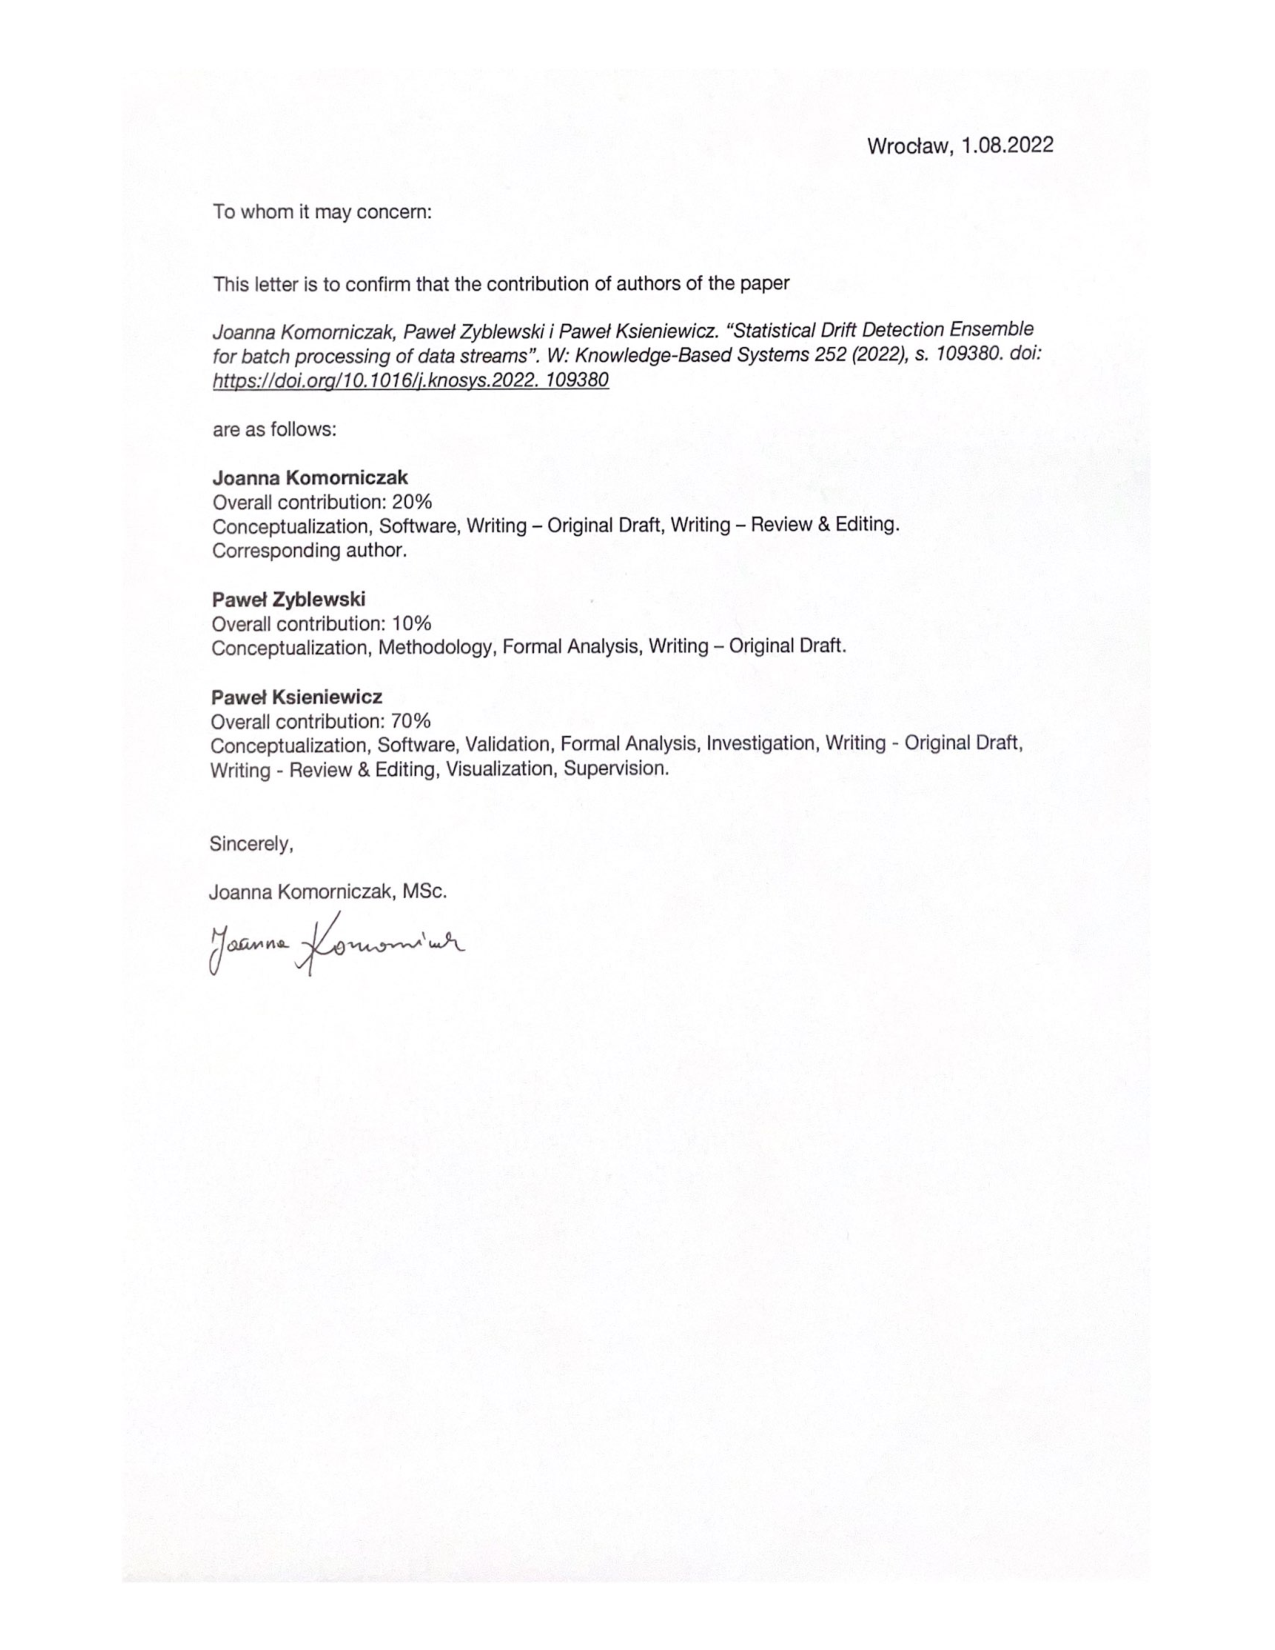
\includepdf[pages=-]{zal/1_JK}
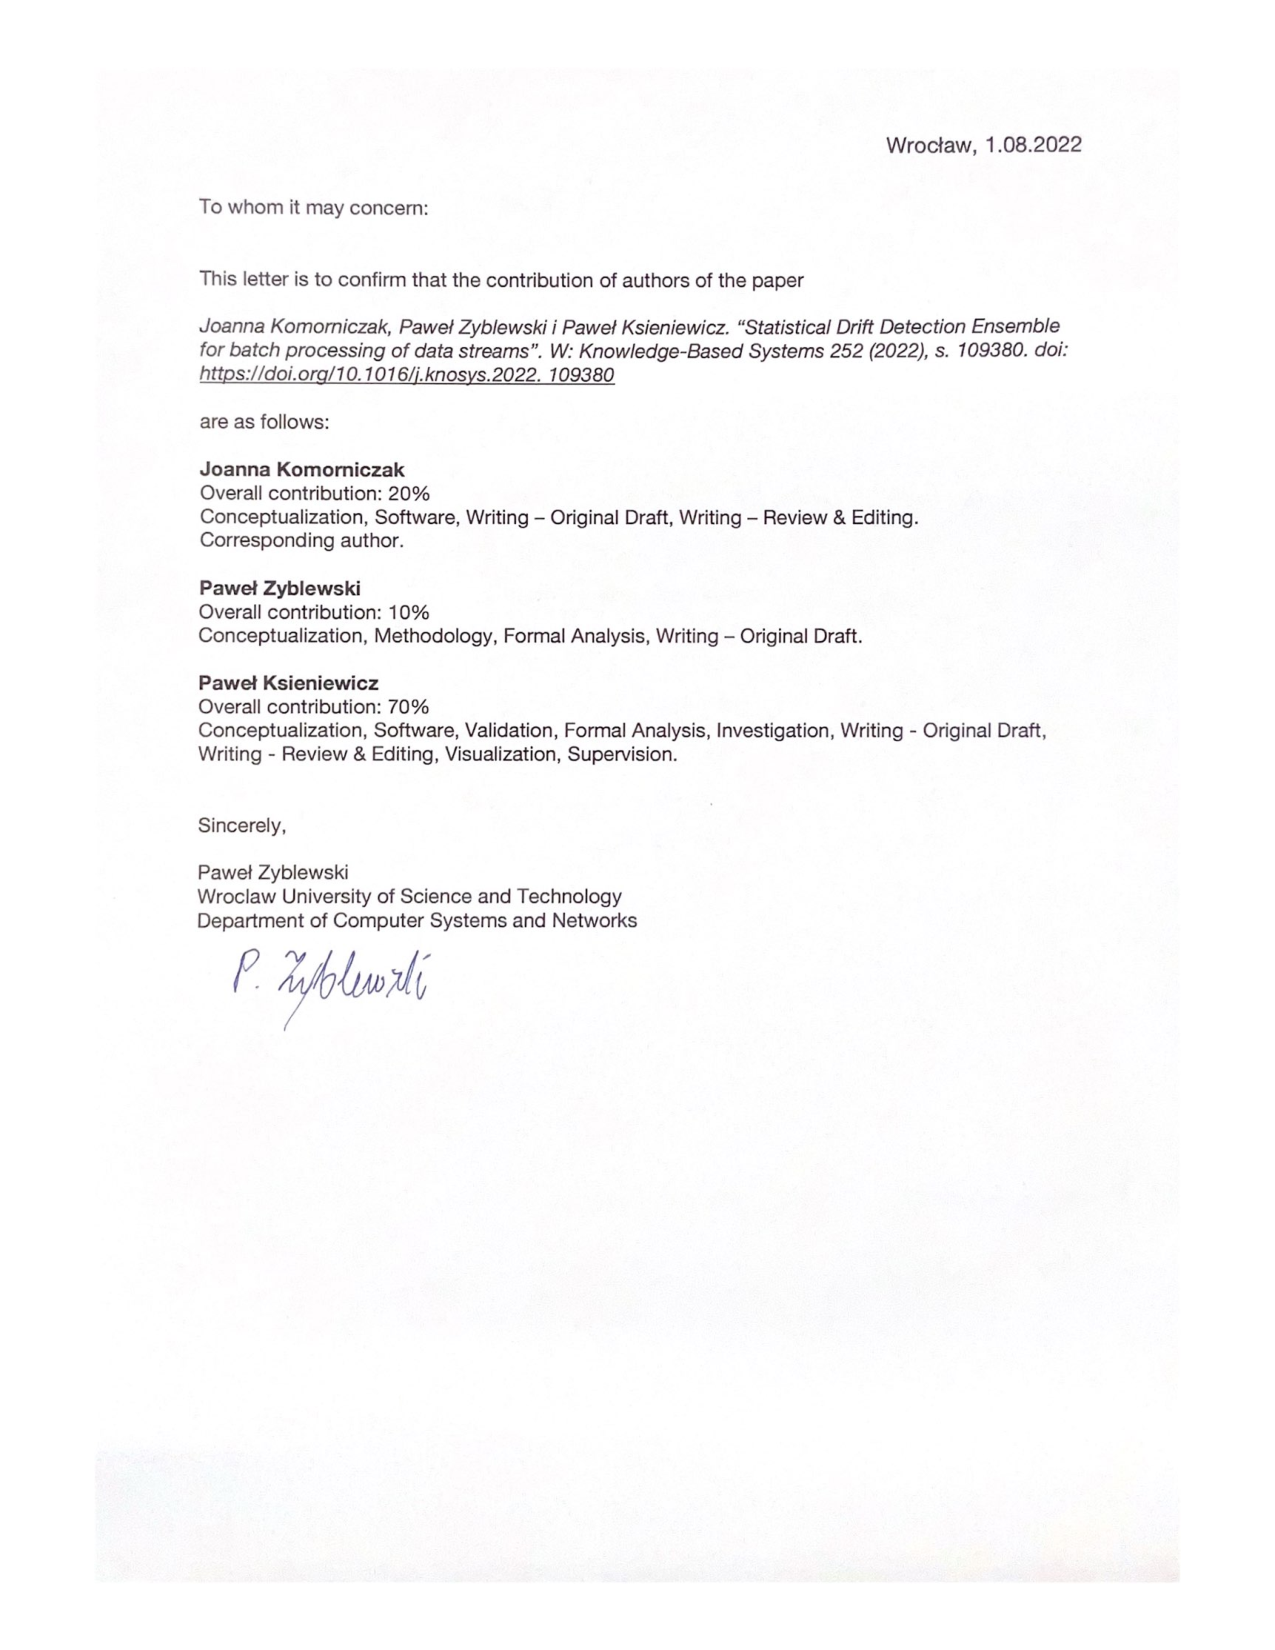
\includepdf[pages=-]{zal/1_PZ}

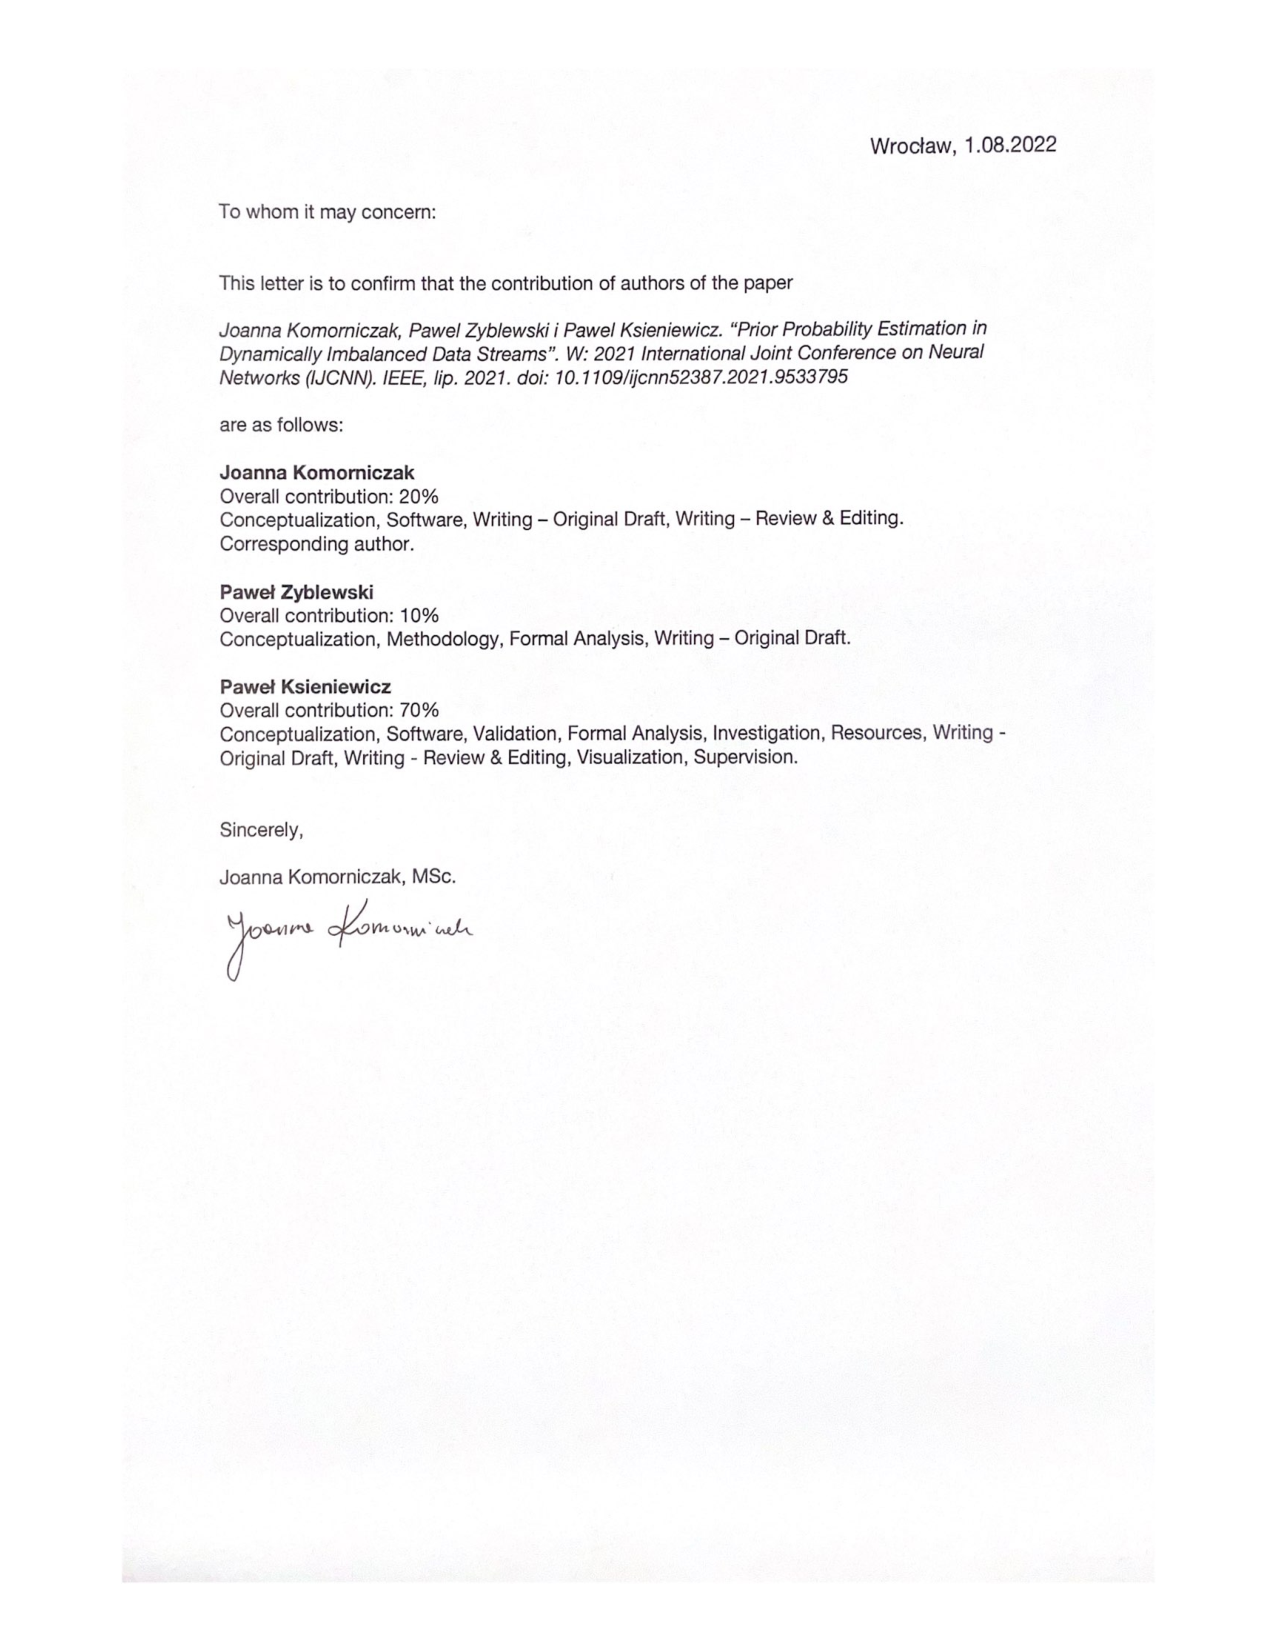
\includepdf[pages=-]{zal/3_JK}
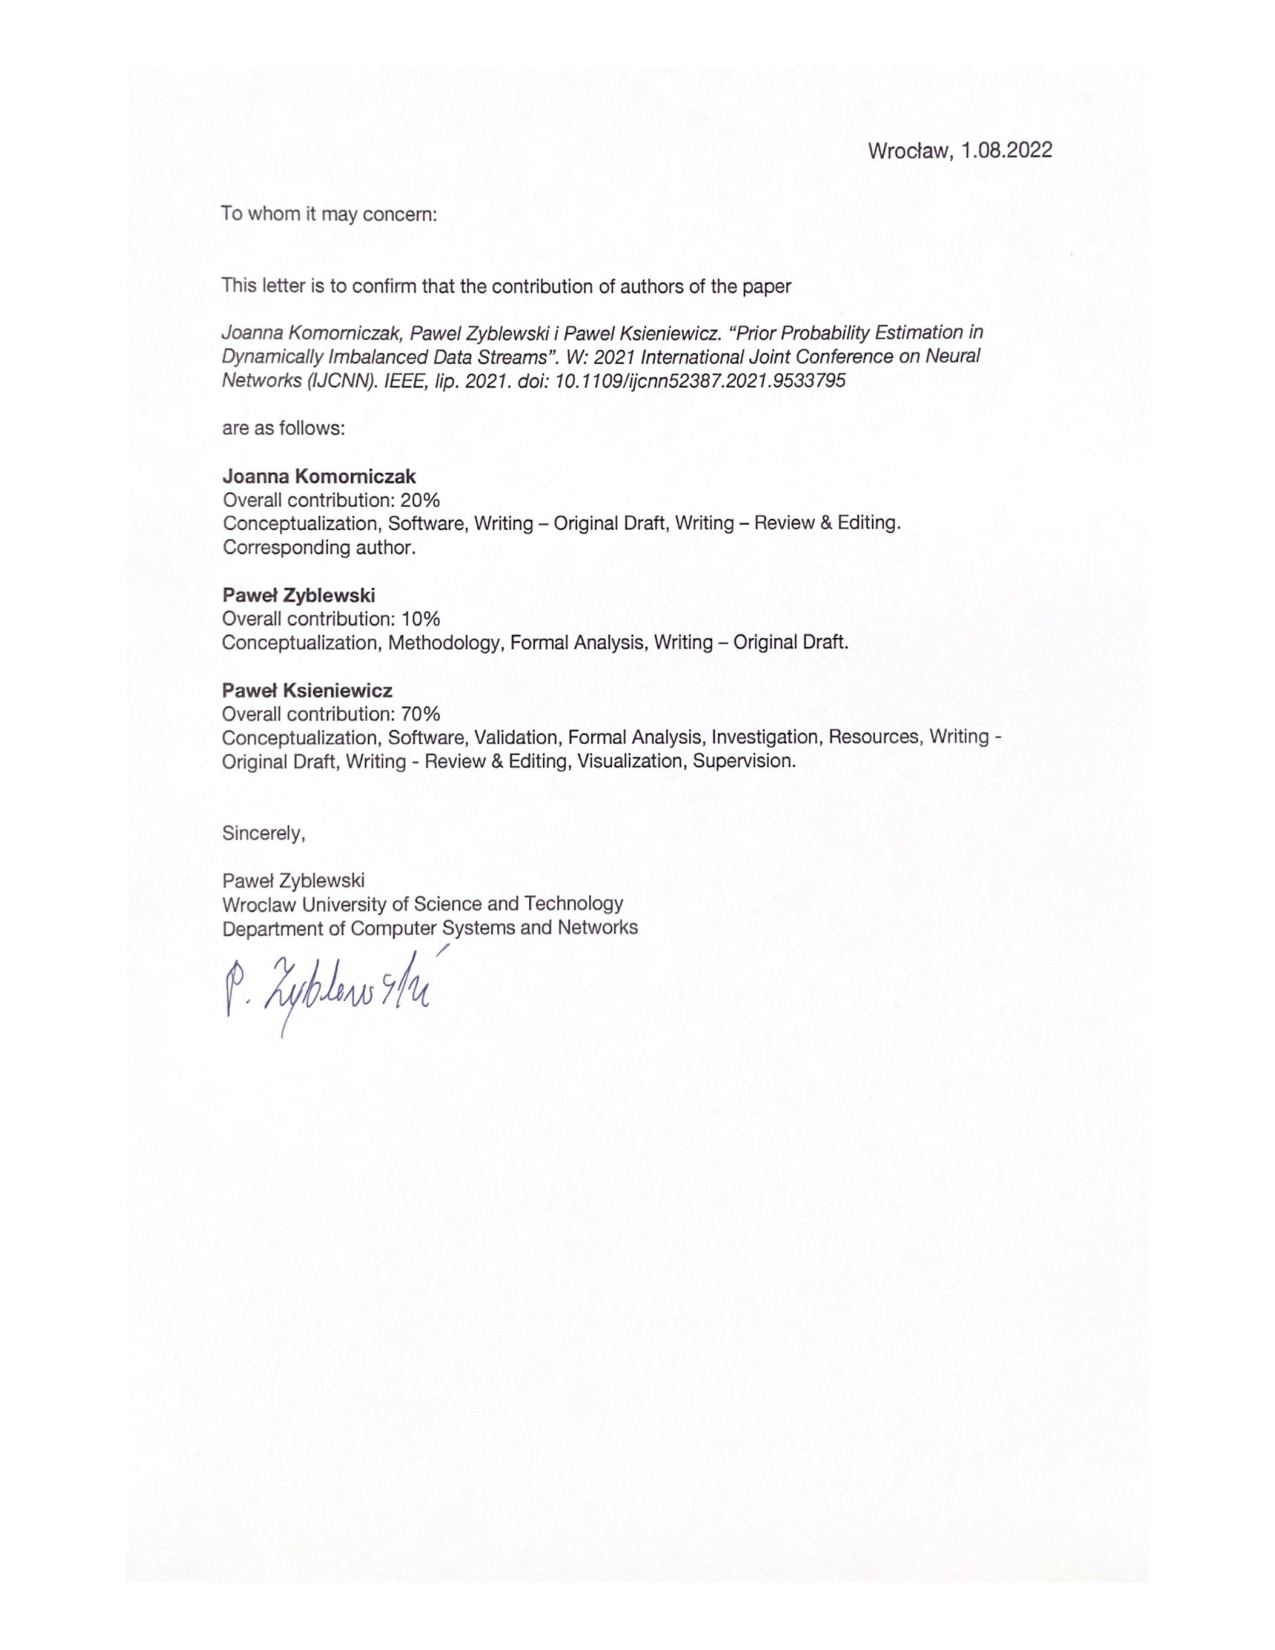
\includepdf[pages=-]{zal/3_PZ}

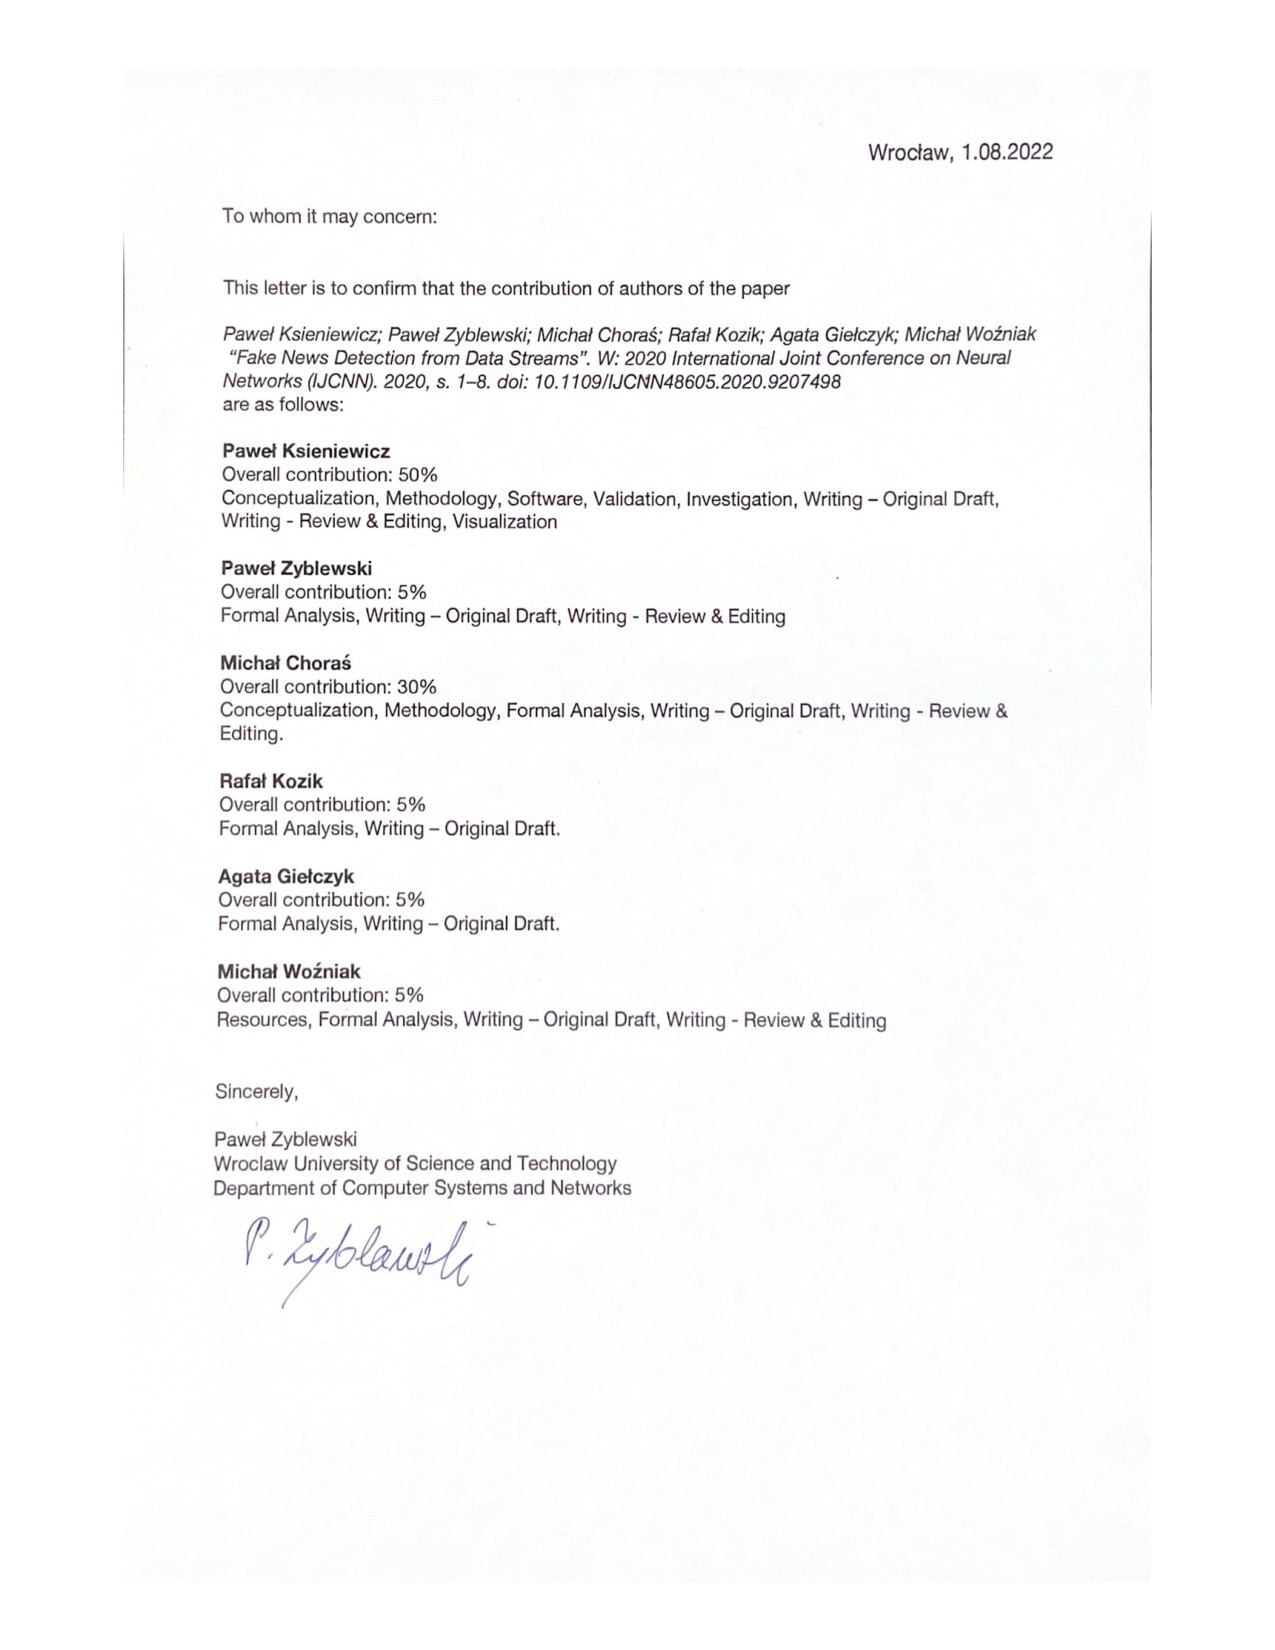
\includepdf[pages=-]{zal/5_PZ}
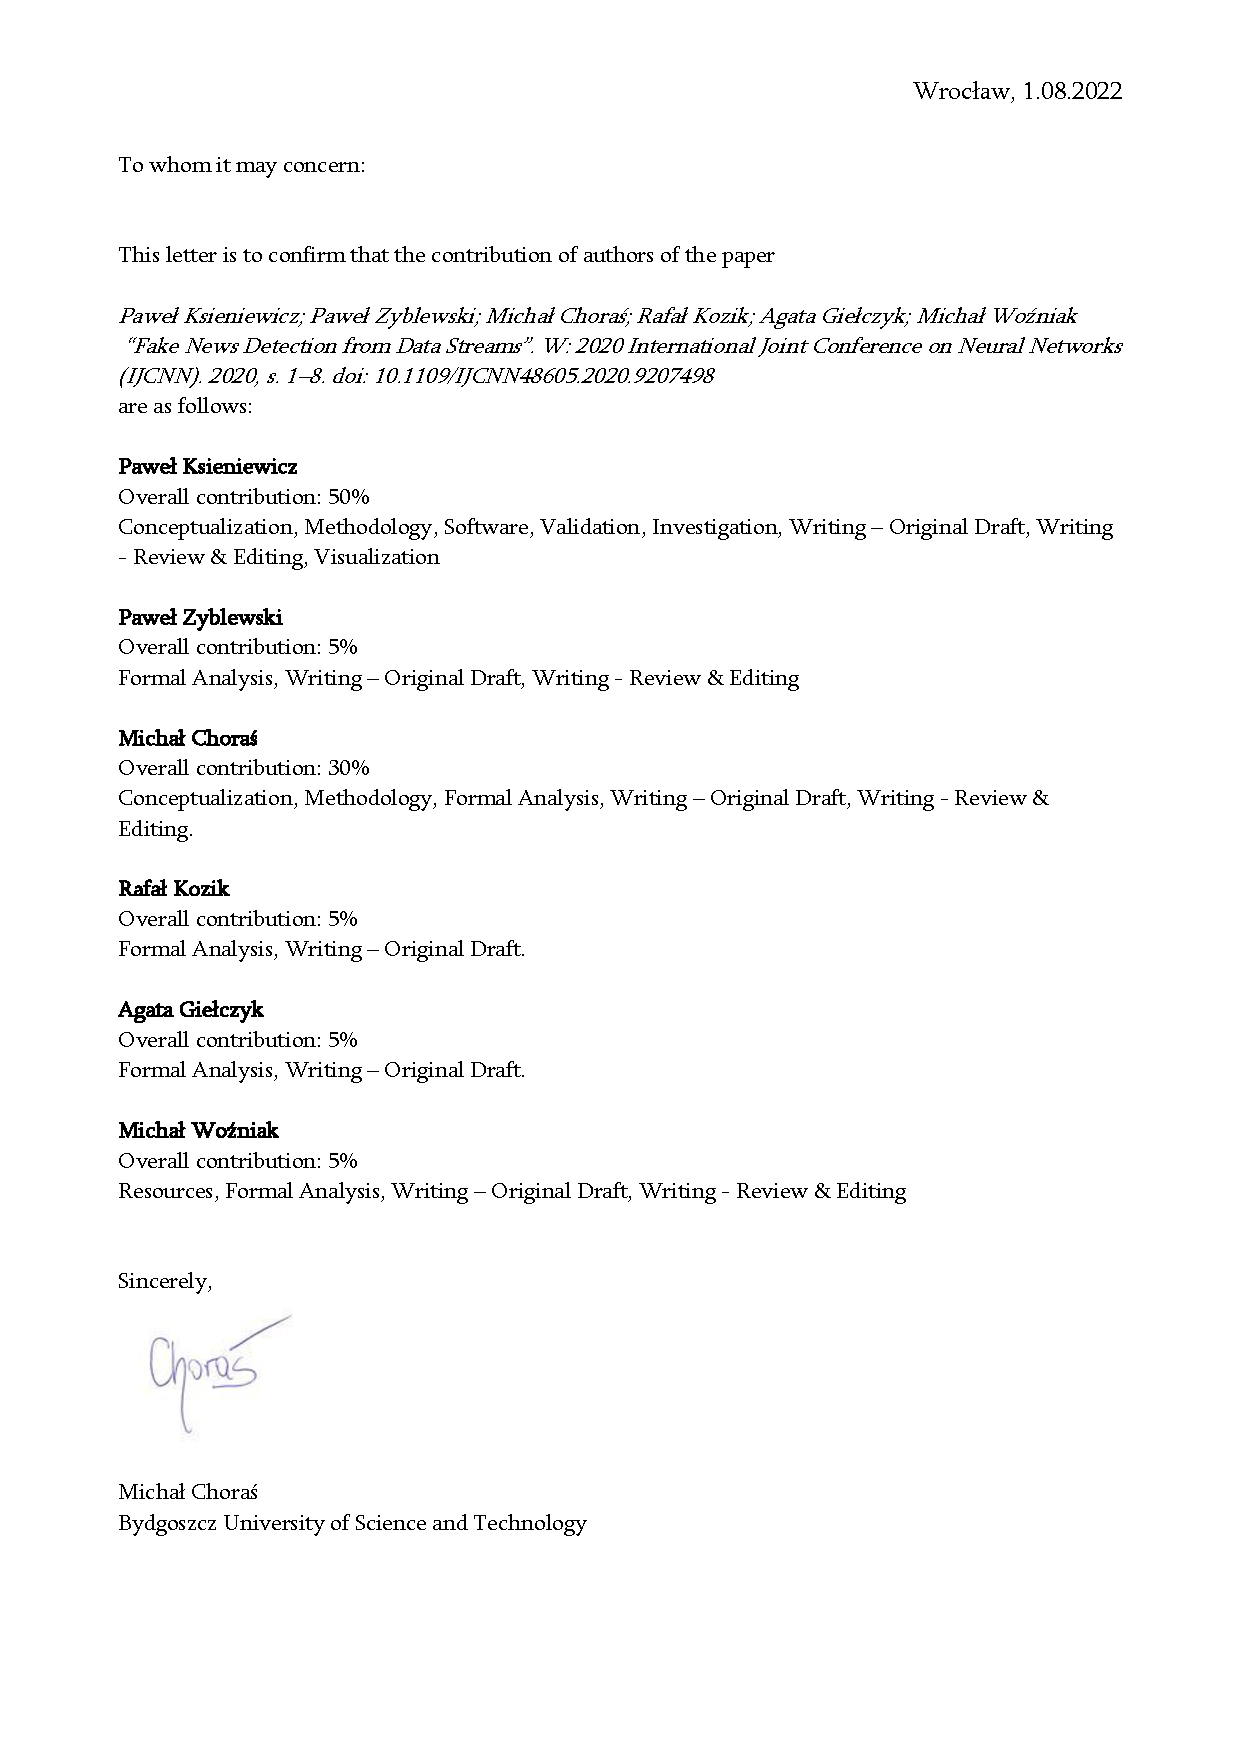
\includepdf[pages=-]{zal/5_MC}
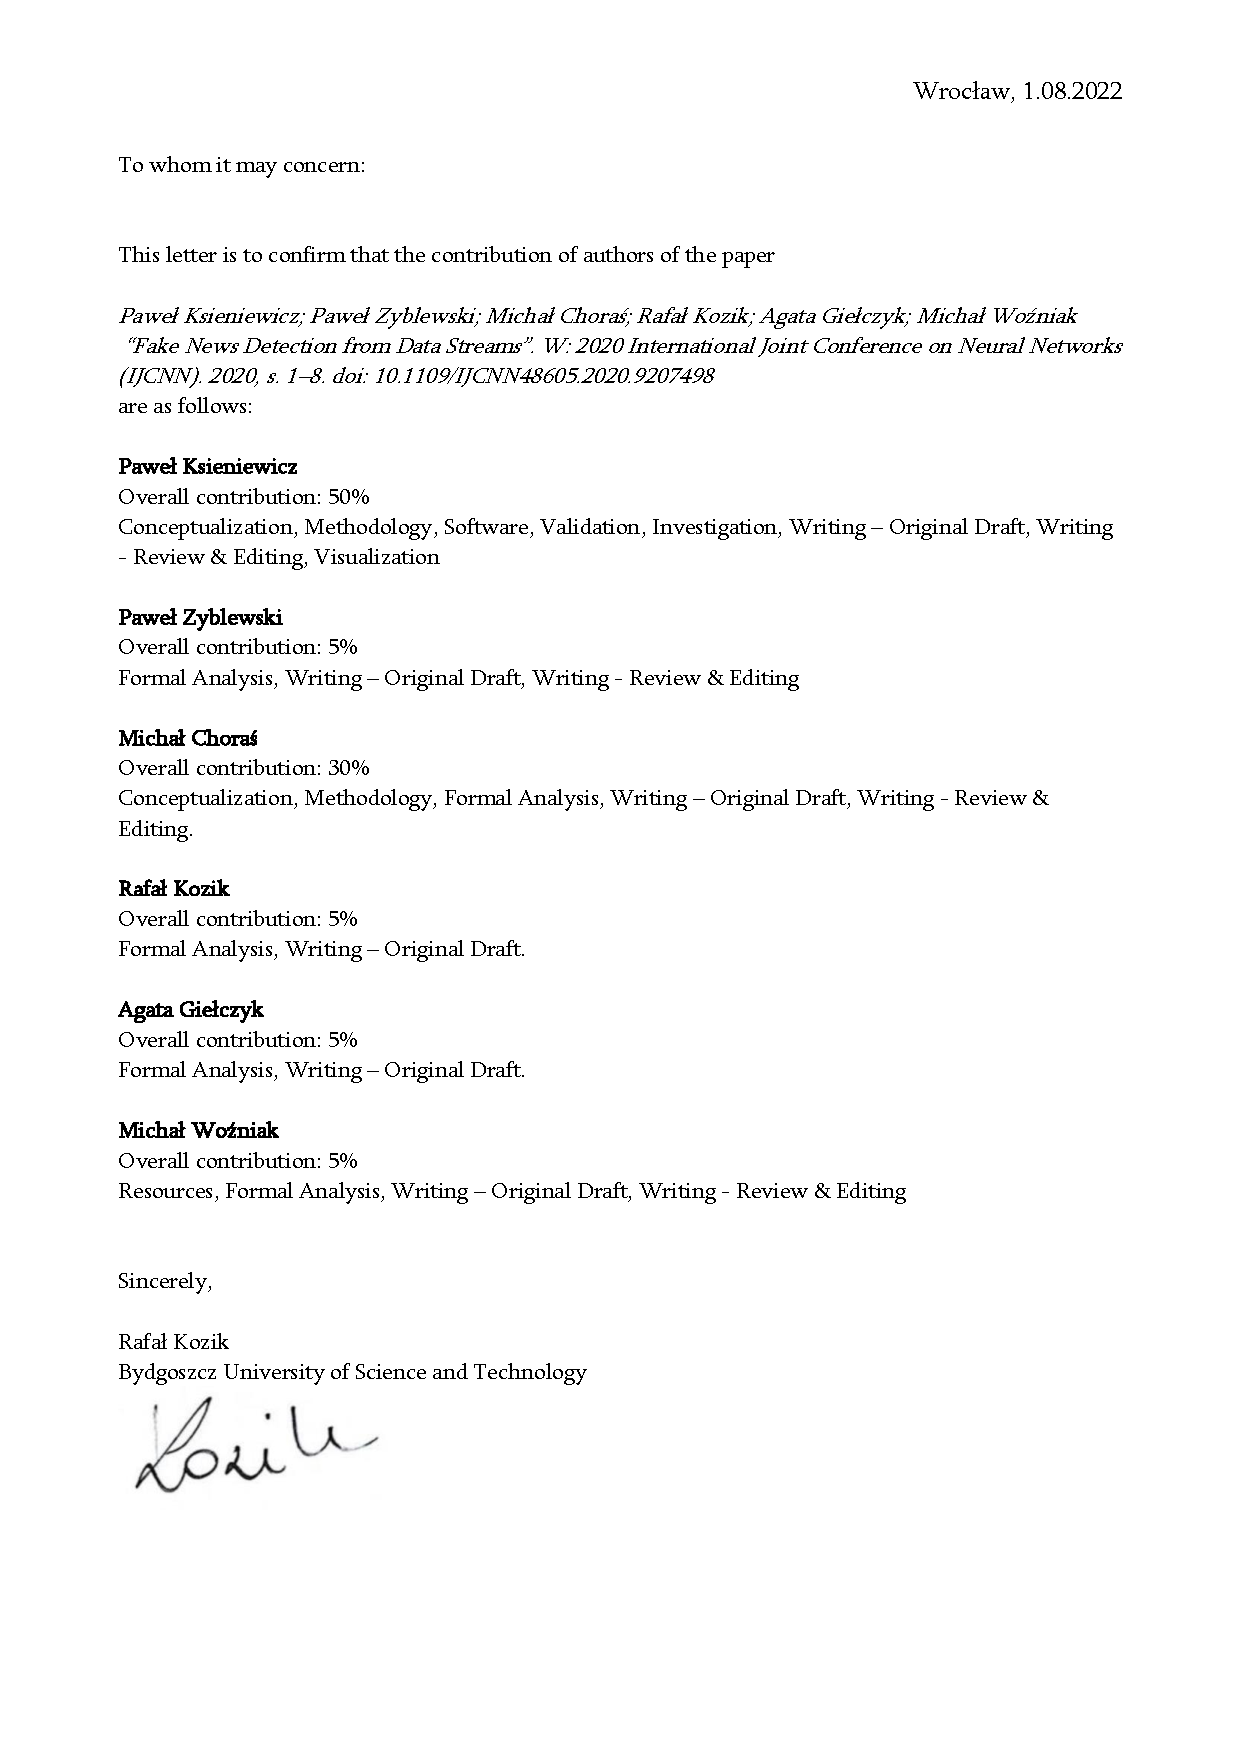
\includepdf[pages=-]{zal/5_RK}
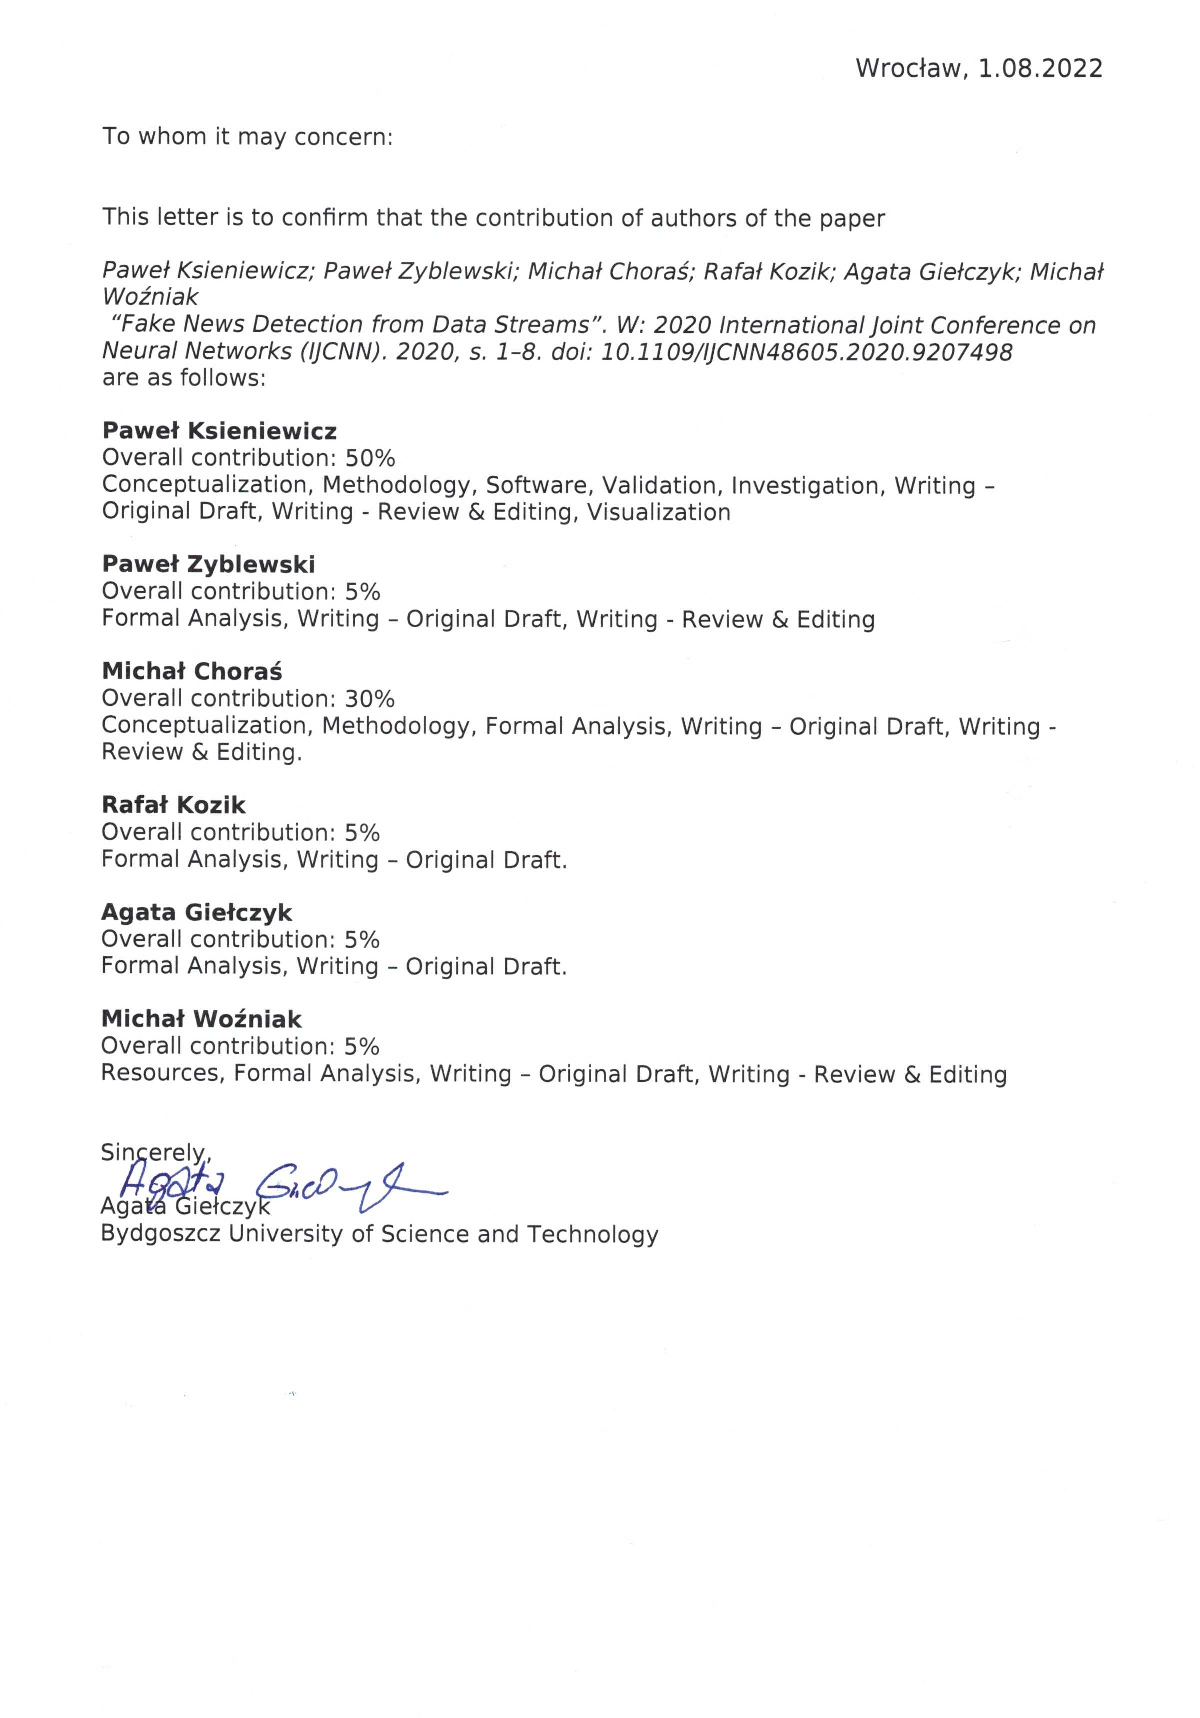
\includepdf[pages=-]{zal/5_AG}
\includepdf[pages=-]{zal/5_MW}

\includepdf[pages=-]{zal/7_MW}
\includepdf[pages=-]{zal/7_BC}
\includepdf[pages=-]{zal/7_AK}
\includepdf[pages=-]{zal/7_KW}

\includepdf[pages=-]{zal/9_MW}

\includepdf[pages=-]{zal/10_BK} % !!
\includepdf[pages=-]{zal/10_MW}

\includepdf[pages=-]{zal/11_MW}

\chapter{Publikacje wchodzące w skład osiągnięcia naukowego}

\begin{fullwidth}

{
\small
\begin{itemize}
	\item[[C1]] \fullcite{C1}
	\item[[C2]] \fullcite{C2}
	\item[[C3]] \fullcite{C3}
	\item[[C4]] \fullcite{C4}
	\item[[C5]] \fullcite{C5}
	\item[[C6]] \fullcite{C6}
	\item[[C7]] \fullcite{C7}
	\item[[C8]] \fullcite{C8}
	\item[[C9]] \fullcite{C9}
	\item[[C10]] \fullcite{C10}
	\item[[C11]] \fullcite{C11}
\end{itemize}	
}
	
\chapter*{\color{red}[C1]\\\fullcite{C1}}
\AddToShipoutPictureBG*{%
  \AtPageLowerLeft{%
    %\vspace*{.5\paperheight}%
    \color{red}%
    \rule{\paperwidth}{.38\paperheight}%
  }%
}
\includepdf[pages=-]{cykl/C1}

\chapter*{\color{red}[C2]\\\fullcite{C2}}
\AddToShipoutPictureBG*{%
  \AtPageLowerLeft{%
    %\vspace*{.5\paperheight}%
    \color{red}%
    \rule{\paperwidth}{.38\paperheight}%
  }%
}
\includepdf[pages=-]{cykl/C2}

\chapter*{\color{red}[C3]\\\fullcite{C3}}
\AddToShipoutPictureBG*{%
  \AtPageLowerLeft{%
    %\vspace*{.5\paperheight}%
    \color{red}%
    \rule{\paperwidth}{.38\paperheight}%
  }%
}
\includepdf[pages=-]{cykl/C3}

\chapter*{\color{red}[C4]\\\fullcite{C4}}
\AddToShipoutPictureBG*{%
  \AtPageLowerLeft{%
    %\vspace*{.5\paperheight}%
    \color{red}%
    \rule{\paperwidth}{.38\paperheight}%
  }%
}
\includepdf[pages=-]{cykl/C4}

\chapter*{\color{red}[C5]\\\fullcite{C5}}
\AddToShipoutPictureBG*{%
  \AtPageLowerLeft{%
    %\vspace*{.5\paperheight}%
    \color{red}%
    \rule{\paperwidth}{.38\paperheight}%
  }%
}
\includepdf[pages=-]{cykl/C5}


\chapter*{\color{red}[C6]\\\fullcite{C6}}
\AddToShipoutPictureBG*{%
  \AtPageLowerLeft{%
    %\vspace*{.5\paperheight}%
    \color{red}%
    \rule{\paperwidth}{.38\paperheight}%
  }%
}
\includepdf[pages=-]{cykl/C6}

\chapter*{\color{red}[C7]\\\fullcite{C7}}
\AddToShipoutPictureBG*{%
  \AtPageLowerLeft{%
    %\vspace*{.5\paperheight}%
    \color{red}%
    \rule{\paperwidth}{.38\paperheight}%
  }%
}
\includepdf[pages=-]{cykl/C7}


\chapter*{\color{red}[C8]\\\fullcite{C8}}
\AddToShipoutPictureBG*{%
  \AtPageLowerLeft{%
    %\vspace*{.5\paperheight}%
    \color{red}%
    \rule{\paperwidth}{.19\paperheight}%
  }%
}
\includepdf[pages=-]{cykl/C8}


\chapter*{\color{red}[C9]\\\fullcite{C9}}
\AddToShipoutPictureBG*{%
  \AtPageLowerLeft{%
    %\vspace*{.5\paperheight}%
    \color{red}%
    \rule{\paperwidth}{.38\paperheight}%
  }%
}
\includepdf[pages=-]{cykl/C9}

\chapter*{\color{red}[C10]\\\fullcite{C10}}
\AddToShipoutPictureBG*{%
  \AtPageLowerLeft{%
    %\vspace*{.5\paperheight}%
    \color{red}%
    \rule{\paperwidth}{.38\paperheight}%
  }%
}
\includepdf[pages=-]{cykl/C10}


\chapter*{\color{red}[C11]\\\fullcite{C11}}
\AddToShipoutPictureBG*{%
  \AtPageLowerLeft{%
    %\vspace*{.5\paperheight}%
    \color{red}%
    \rule{\paperwidth}{.19\paperheight}%
  }%
}
\includepdf[pages=-]{cykl/C11}

\end{fullwidth}



%%
% The back matter contains appendices, bibliographies, indices, glossaries, etc.

\backmatter

%\bibliography{sample-handout}
%\bibliographystyle{plainnat}

%\bibliography{bibliography}
%\bibliographystyle{plainnat}

%\printindex


\end{document}
